\documentclass[11pt]{article}
\usepackage{amsfonts,amsmath,amssymb,amsthm}
\usepackage{graphicx,psfrag,epsf}
\usepackage{enumerate}
\usepackage{url} 
\usepackage{algorithm}
\usepackage{algpseudocode}
\usepackage{authblk}
\usepackage{helvet}
\usepackage[colorlinks=true,pagebackref,linkcolor=magenta]{hyperref}
\usepackage[sort&compress,comma,square,numbers]{natbib}
\usepackage{fullpage,fancyhdr}
\renewcommand{\familydefault}{\sfdefault}
\usepackage{color} 
\usepackage{paralist}
\usepackage{lineno}
\usepackage[font=small,labelfont=bf]{caption}
\usepackage[final,authormarkup=none]{changes}
\newcommand{\note}[2][]{\added[#1,remark={#2}]{}}
\definecolor{green}{rgb}{0.1840,0.4362,0.1003} 

\usepackage{tikz}
\usepackage{graphicx}
\usetikzlibrary{calc}

\pagestyle{fancy}
\textwidth=6.5in
\headwidth=6.5in
\textheight=9.0in
\headheight=0.0pt
\topmargin=0.0in
\headsep=0.0in
\renewcommand{\headrulewidth}{0pt}

\setlength{\parindent}{0em}
\setlength{\parskip}{0.7em}

\providecommand{\sct}[1]{{\normalfont\textsc{#1}}}
\providecommand{\mt}[1]{\widetilde{#1}}
\providecommand{\mb}[1]{\boldsymbol{#1}}
\providecommand{\mc}[1]{\mathcal{#1}}
\newcommand{\Real}{\mathbb{R}}
\newcommand{\G}{c}
\newcommand{\K}{\mathcal{K}}
\newcommand{\LL}{\mathcal{L}}
\newcommand{\Migraine}{\sct{Migraine}}
\newcommand{\mtg}{\sct{m2g}}
\newcommand{\T}{^{\ensuremath{\mathsf{T}}}}           % transpose
\newcommand{\Linefor}[2]{%
    \State \algorithmicfor\ {#1}\ \algorithmicdo\ {#2} \algorithmicend\ \algorithmicfor%
}
\newcommand{\Lineif}[2]{%
    \State \algorithmicif\ {#1}\ \algorithmicdo\ {#2} \algorithmicend\ \algorithmicif%
}

\normalem
\newcommand{\Mgc}{\sct{Mgc}}
\newcommand{\Mgcp}{\sct{Mgc$_P$}}
\newcommand{\Mgcd}{\sct{Mgc$_D$}}
\newcommand{\Mgcm}{\sct{Mgc$_M$}}
\newcommand{\Hhg}{\sct{Hhg}}
\newcommand{\Dcorr}{\sct{Dcorr}}
\newcommand{\Mcorr}{\sct{Mcorr}}
\newcommand{\Mantel}{\sct{Mantel}}

\newcommand{\website}{\url{https://github.com/neurodata/MGC/}}

\newcommand{\jv}[1]{{\note{jv: #1}}}
\newcommand{\cs}[1]{{\note{cs: #1}}}

\newcommand{\mbx}{\ensuremath{\mb{x}}}
\newcommand{\mby}{\ensuremath{\mb{y}}}
\newcommand{\rto}{\leftarrow}
\newcommand{\argmax}{\operatornamewithlimits{argmax}}
\newcommand{\argmin}{\operatornamewithlimits{argmin}}

\newtheorem{thm}{Theorem}
%\newtheorem{appThm}{Theorem}
%\setcounter{appThm}{0}
\newtheorem{lem}{Lemma}
%\newtheorem{appLem}{Lemma}
%\setcounter{appLem}{0}
\newcommand*\mean[1]{\bar{#1}}

\renewcommand{\algorithmicrequire}{\textbf{Input:}}
\renewcommand{\algorithmicensure}{\textbf{Output:}}

\pagenumbering{arabic}
\linenumbers


\begin{document}

\def\spacingset#1{\renewcommand{\baselinestretch}%
{#1}\small\normalsize} \spacingset{1}

\title{\bf Discovering Relationships Across Disparate Data Modalities}
\author[1,2]{Cencheng Shen} %\thanks{cshen6@jhu.edu}}
\author[1,3]{Carey E. Priebe}% \thanks{cep@jhu.edu}}
\author[3,4,6]{Mauro Maggioni}%\thanks{mauro.maggioni@jhu.edu}}
\author[1,5,6,7]{Joshua T. Vogelstein\thanks{jovo@jhu.edu}}
\affil[1]{Center for Imaging Science, Johns Hopkins University}
\affil[2]{Department of Statistics, Temple University}
\affil[3]{Department of Applied Mathematics and Statistics, Johns Hopkins University}
\affil[4]{Department of Mathematics, Johns Hopkins University}
\affil[5]{Department of Biomedical Engineering and Institute for Computational Medicine, Johns Hopkins University}
\affil[6]{Institute for Data-Intensive Engineering \& Science, Johns Hopkins University}
\affil[7]{Institute for Computational Medicine, Johns Hopkins University}
\maketitle

% \bigskip
\begin{abstract}
% \jv{all of science seems limiting}
Discovering whether certain properties are associated with other properties is fundamental to all science.
As the amount of data increases, it is becoming increasingly difficult and important to determine whether one property of the data (e.g., cloud shape) is related to another (e.g., grass wetness).  Only If they are related does it make sense to further investigate the nature of the relationship. Previous work stuggles to reliably identifying relationships when the properties are complex and high-dimensional and the relationship is nonlinear. 
We conjectured that these limitations stem from those methods being ``global'' techniques, meaning that they search for global structure.
We build  on recent advances in nonlinear function estimation, by providing the first statistically principled and computationally efficient methodology for finding the optimal scales.  
We show that Multiscale Generalized Correlation (\Mgc) is as good as (in linear settings) and often better than (in high-dimensional and nonlinear settings) the previously proposed global methods. 
Moreover, we demonstrate that \Mgc~is the only dependence test that can provide insight into the nature of dependence.
We apply \Mgc~to detect the presence and investigate the nature
of the relationships between brain activity and personality, brain shape and disorder, and  brain connectivity and creativity. We additionally illustrate that \Mgc~does not suffer from the false positive inflation problem that has plagued parametric methods.  Our open source implementation of \Mgc~is easy to use and applicable to fundamental questions confronting science, government, finance, and many other disciplines. 
\end{abstract}


\noindent%
{\it Keywords: testing independence, distance correlation, k-nearest-neighbor, kernel test, permutation test}

\clearpage
\setcounter{tocdepth}{2}

Identifying the existence of a relationship is a precursor to investigating the structure of the relationship,  whether it has predictive power, and whether it reflects causality.
One of the first statistical approaches to determine whether two properties are related to---or statistically dependent on---one another is Pearson's Product-Moment Correlation (published in 1895 \cite{Pearson1895}). This seminal paper prompted the development of  entirely new ways of thinking about and quantifying relationships (see \cite{Reimherr2013,JosseHolmes2013} for  recent reviews and discussion).


Modern datasets, however, present particularly vexing challenges for dependence-testing that were not foreseen in Pearson's era.
%
First, the dependencies between different properties 
of data can be highly \textbf{nonlinear}.
% 
Second, the \textbf{dimensionality} of individual samples is growing at exponential rates, with genomics and connectomics datasets, for example, often encompassing millions or even billions of dimensions. 
%
Third, the \textbf{sample sizes} are not increasing proportionally, meaning that we are often confronted with ultrahigh-dimensional datasets derived from relatively few samples.
% 
Fourth, the data are often \textbf{structured}---sequences, images, networks, shapes, and text---creating problems for standard methods that were developed for unstructured feature sets.
% 
Fifth, because of the continuing data deluge,  \textbf{computationally efficient} methods are critical for generating results within acceptable time frames.
%
And finally, we not only want to know \textit{whether}  properties are dependent on each other, but also \textit{how} they are related.
There is thus a  need for a method that satisfactorily address all of these challenges that is supported by compelling evidence for its theoretical efficacy and practical utility.


To illustrate these challenges, consider the following simple example.
Suppose we wish to determine whether there is a relationship between cloud shape and the wetness of the ground under those clouds.  We  record observations of cloud shape and ground wetness on 50 different days.
  Let $x_i$ denote cloud shape on day $i$ and $y_i$ denote ground wetness on that same day. 
If the relationship between cloud shape and ground wetness is approximately linear, the data might look like the top row in Figure \ref{f:newschem}. 
On the other hand, if the relationship is a spiral, it might look like
like those in the bottom row of Figure \ref{f:newschem}.
% For either case, we illustrate our four-step approach to detect dependence and reveal its nature by Multiscale Generalized Correlation. (see Algorithm \ref{alg:mgc} in Appendix \ref{appen:algorithms} for pseudocode).


All dependence tests that can detect arbitrary relationships compute the distances between all pairs of objects \emph{within} each property \cite{SzekelyRizzo2009,SzekelyRizzo2013b,HellerGorfine2013}. Thus, given $n=50$ observations, they compute $n \times n$ distances for property $x$, and another $n \times n$ distances for property $y$. 
% Thre needs to be another sentence here.  Something like "If the shape of the cloud on day 7 is more like the shape of the cloud on day 43 than on any other day, we then focus our attention on the ground wetness on days 7 and 43.  Such a pair-wise comparison is very different fro standard comparisons in which the cloud density and ground wetness on day 7 are blah blah because I don't know how best to distinguish pairwise from stndard comparisons.  You do, though.     Pairwise comparisons have 
Operating on comparisons between pairs of observations has a rich history in statistics and machine learning, including Mantel's dependence test \cite{Mantel1967} and  kernel methods \cite{scholkopf2002learning}.
% , and certain manifold learning techniques \cite{
% TorgersonBook, 
% TenenbaumSilvaLangford2000, 
% SaulRoweis2000, 
% BelkinNiyogi2003,
% DiffusionPNAS}.
The popularity of pairwise comparisons rests on two properties. 
First, comparisons can be easily defined on any kind of data, including structured objects like shapes and text.  This is in contrast to say, a t-test, which requires scalar numbers.  
Second, pairwise comparisons have been shown to be sufficient statistics in a variety of contexts, including testing for equality of distributions \cite{Maa1996}, 
% manifold learning \cite{RoweisSaul2003,MMS:NoisyDictionaryLearning}, 
and dependence testing \cite{SzekelyRizzo2009,SzekelyRizzo2013b}. 
% 
However, existing tests struggle in
% The second step is where other approaches, such as the celebrated ``distance correlation'' (\Dcorr) break down for 
nonlinear or high-dimensional settings with low sample sizes \cite{SzekelyRizzo2009,HellerGorfine2013}. We conjecture this is because existing tests are effectively looking for global nonlinear structure; whereas local linear structure is both statistically and computationally easier to detect.

To mitigate this challenge, we therefore look to a different sub-field of data science that has utilized the ``principle of locality''.  Under this principle, rather than using all the data to discover global structure, methods only use data samples that are ``close'' to one another to find local structure. This strategy  has reaped considerable benefits in a wide range of data science problems, including  classification and regression  \cite{Stone1977}, data compression \cite{DaubechiesWaveletBook},  recommender systems \cite{Sarwar2000}, and even testing \cite{David1966,Friedman1983,Schilling1986}.
Moreover, it has become an invaluable tool in unfolding nonlinear geometry in many nonlinear dimensionality reduction (or manifold learning) algorithms (for example, \cite{
TorgersonBook, 
TenenbaumSilvaLangford2000, 
SaulRoweis2000, 
BelkinNiyogi2003,
DiffusionPNAS,
MMS:NoisyDictionaryLearning}). 
However, all of these approaches have been plagued by having to choose the optimal scale.  More specifically, each approach must choose a threshold, such that all within that threshold are considered local, and all those outside that threshold are effectively ignored.  
Without guidance, these tools rely on costly cross-validation techniques and other heuristics to choose the optimal scale.

Our key insight is that we can determine the optimal scale using a statistically consistent and computational efficient manner.  



% Our approach, 
% \emph{Multiscale Generalized Correlation} (\Mgc), mitigates this challenge. 
Specifically, rather than  computing the correlation between all pairs of distances at the second step, we compute the correlation between subsets of pairs of distances as follows.
For each point, \Mgc~finds its nearest neighbor in $x$ and its nearest neighbor in $y$, and computes the distance only between those neighboring points, and then computes the correlation only among those local distances.  Then, \Mgc~iteratively increases the number of neighbors of $x$ to include, as well as those for $y$, for each computing  the linear correlation only between those local distances.   

% \Dcorr~computes the correlation between all pairs of distances (see Appendix \ref{appen:dcorr} for details). 
% When the relationship is nearly linear, samples that are close in $x$ are also close in $y$ (see points marked $1$ and $2$). 
% However, when the relationship is nonlinear, there may be many points that are close in $y$ but not $x$  (see points marked $2$ and $3$).  
% Thus, computing the linear correlation for all pairs of distances will include many distance pairs that decrease the distance correlation, making the two properties seemingly unrelated in the \Dcorr~test."

Doing so for all possible ``scales'' (or neighborhood sizes) yields a \emph{multiscale correlation map}. 
This approach is an explicit generalization of previous work which only consider a single scale---the global one---consisting of all pairs of observations. 
Given this multiscale map, \Mgc~searches for the best test statistic, $c^*$, that is, the largest test statistic after smoothing to address sample noise (see Algorithm \ref{alg:sample_mgc} for details). 

\begin{figure}
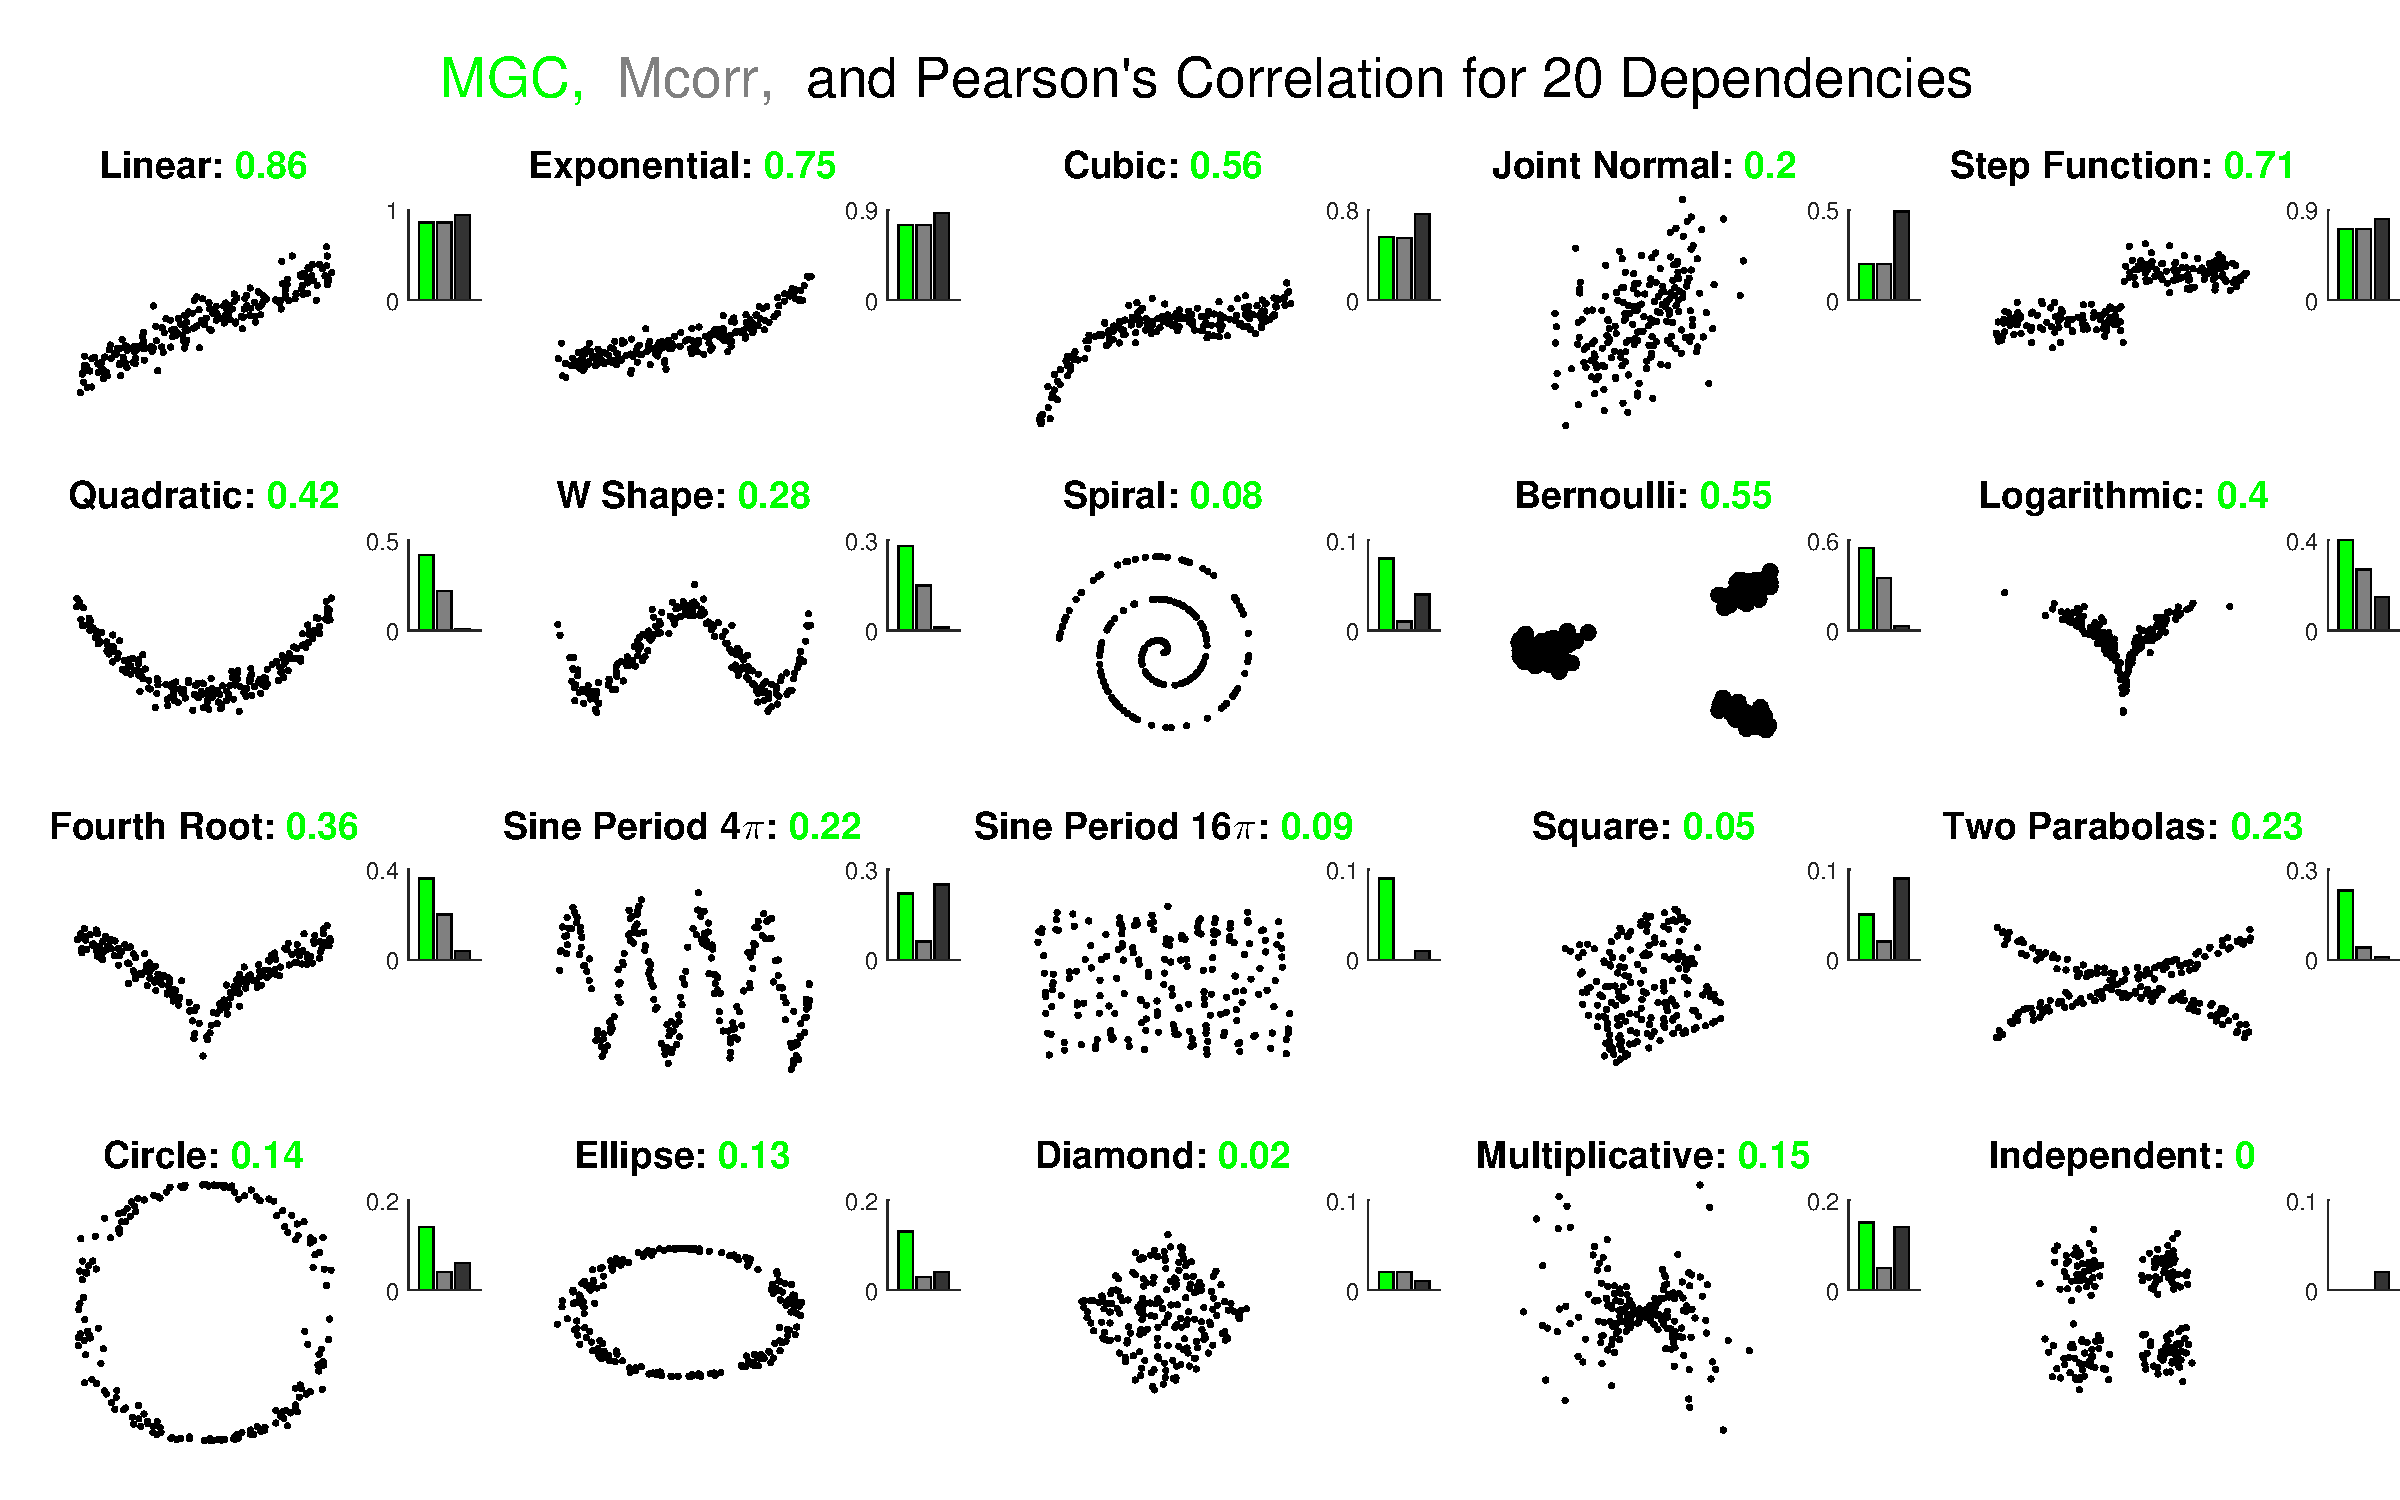
\includegraphics[width=1.0\textwidth,trim={0cm 0cm 0cm 0cm},clip]{Figures/FigSimVisual2.pdf}
\caption{candidate figure: This figure shows that \Mgc~is a superior correlation measure for dependence, as \Mgc~yields a correlation measure larger than $0$ for all types of dependencies while being $0$ under independence. In comparison, \Dcorr~can be very close to $0$ for many nonlinear dependencies, despite it is a consistent statistic for testing dependence; and pearson's correlation is a correlation measure for linear association rather than dependence, such that it also fails to capture many nonlinear dependencies. For each relationship, the \Mgc~statistic is shown above; and the accompanying chart bar compares \Mgc~(green), \Mcorr~(gray), and pearson's correlation in the absolute value (black), all of which lie in the range of $[0,1]$ with $0$ indicating no relationship. The detailed settings are in Supplementary~\ref{appen:function}, for which we set sample size $n=200$ and the noise level at $0.2$, randomly generate sample observations pairs, and calculate each correlation measure.}
\end{figure}

\begin{figure}
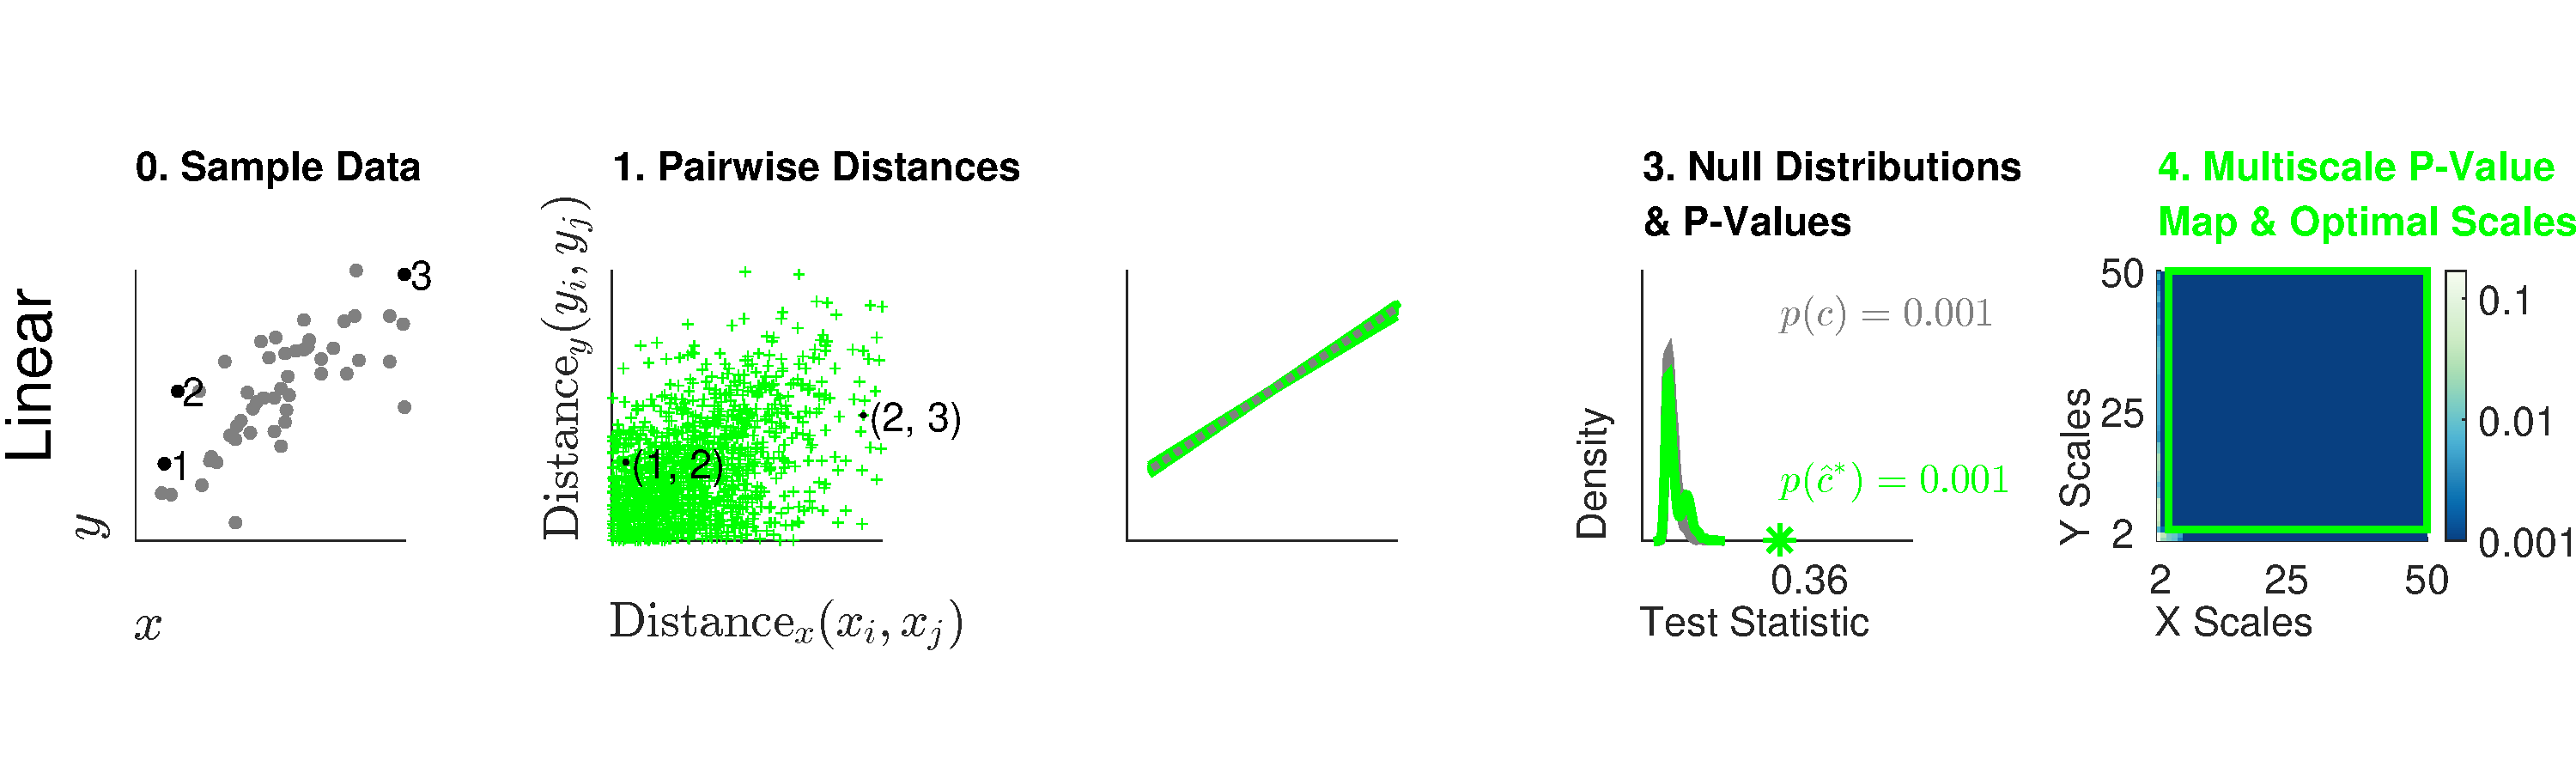
\includegraphics[width=1.0\textwidth,trim={0cm 1.5cm 0cm 2.5cm},clip]{Figures/A2_type1_n50_noise5.pdf}
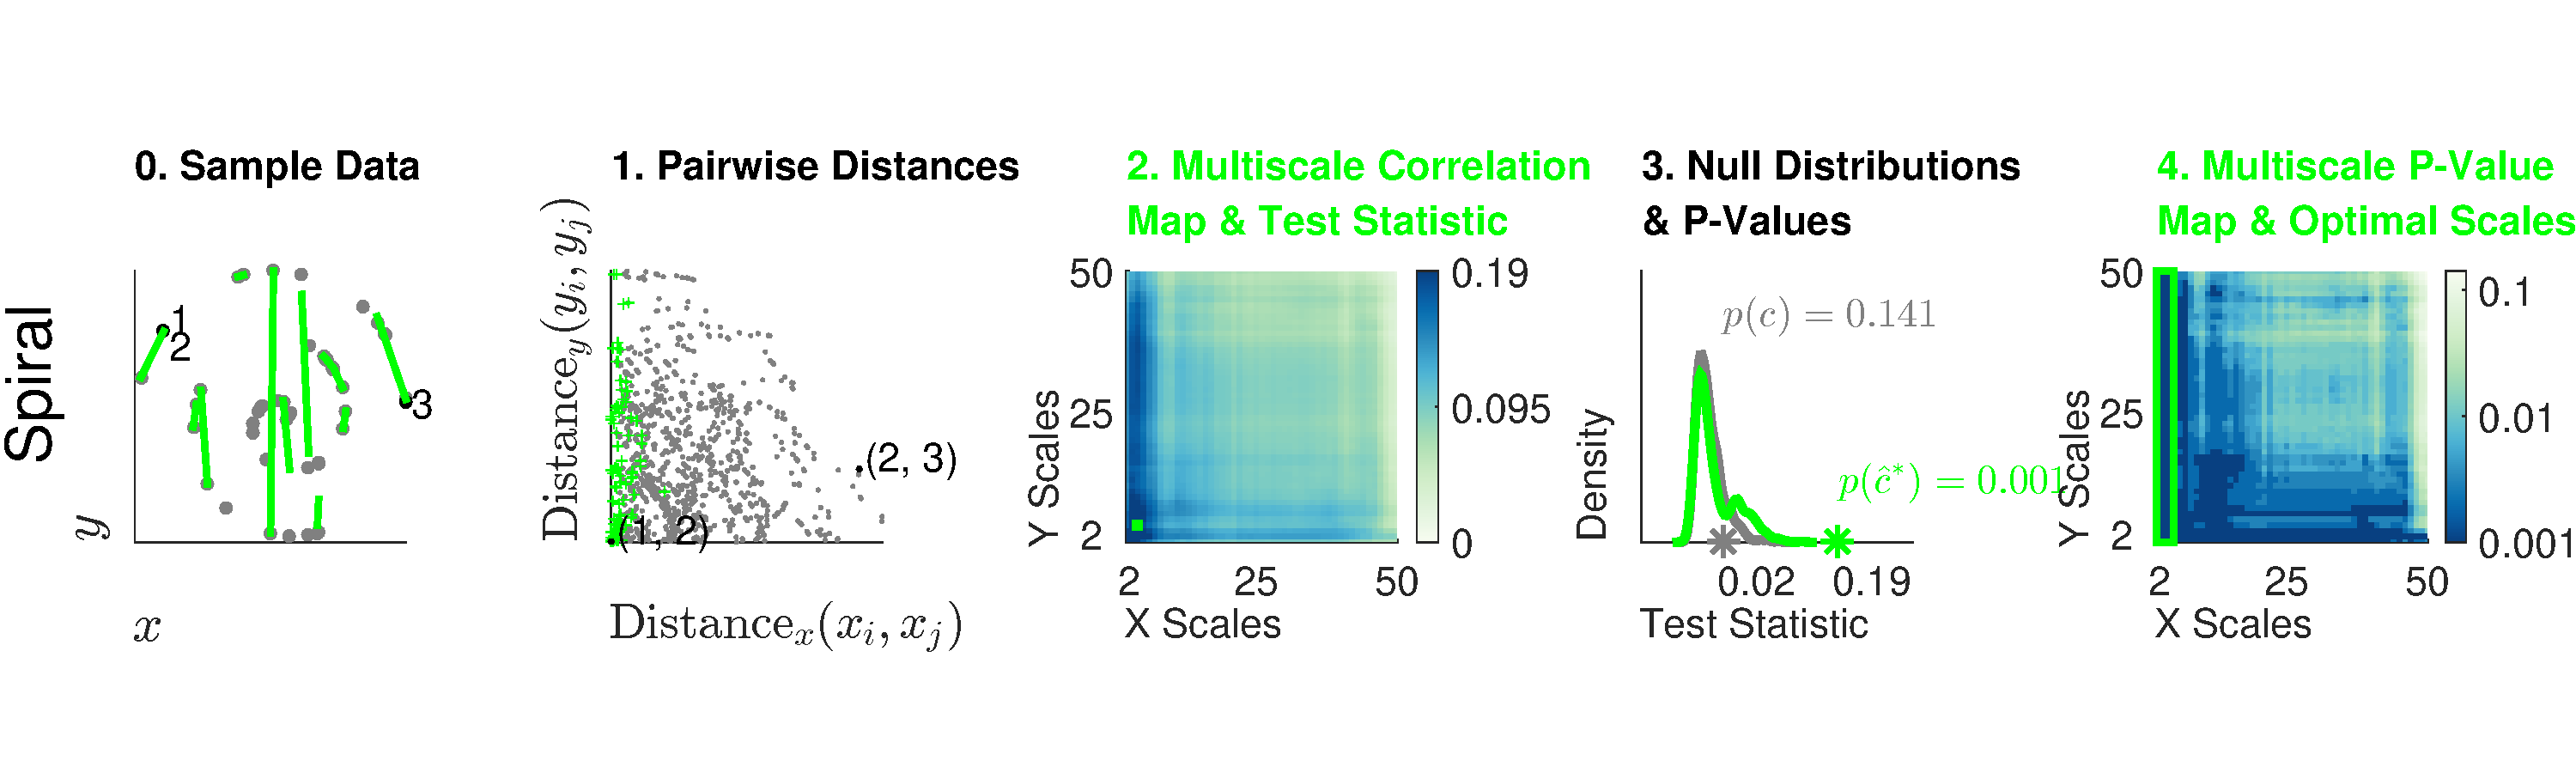
\includegraphics[width=1.0\textwidth,trim={0cm 1.5cm 0cm 5cm},clip]{Figures/A2_type8_n50_noise0.pdf}
\caption{Candidate figure}
\end{figure}

\begin{figure}
% 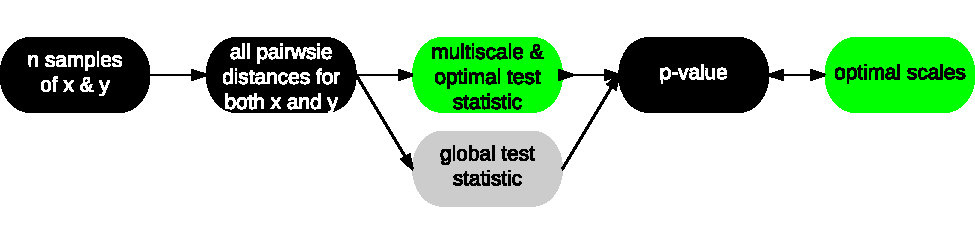
\includegraphics[width=1.0\textwidth]{Figures/flowchart}
% trim={<left> <lower> <right> <upper>}
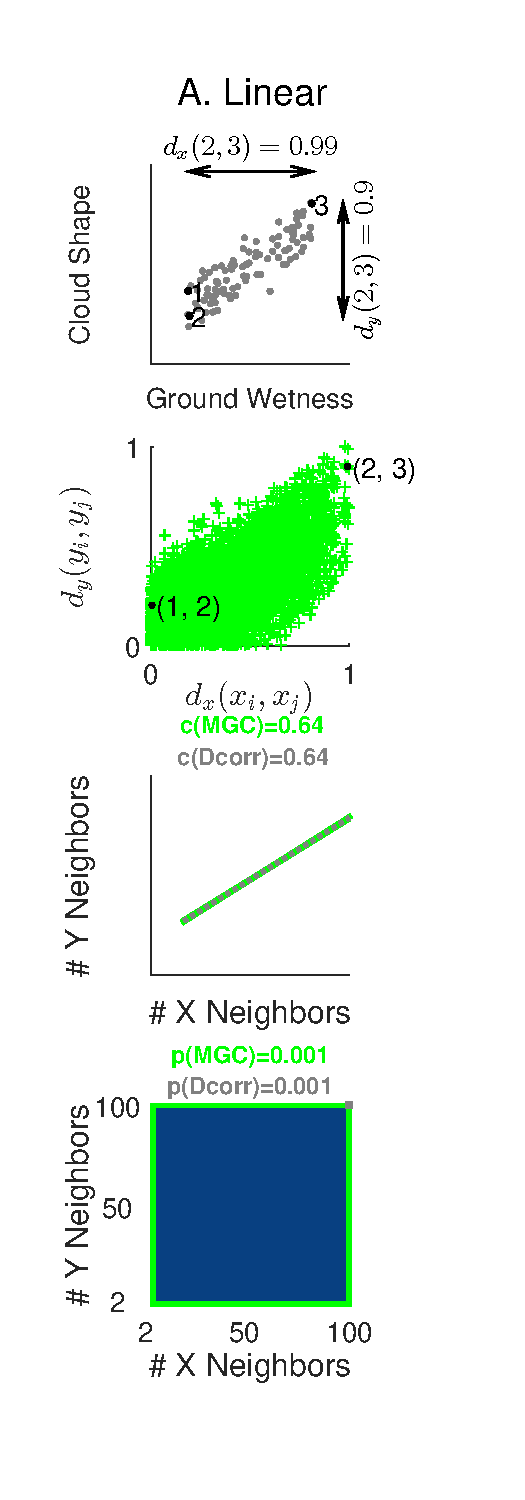
\includegraphics[width=1.0\textwidth,trim={0cm 1.5cm 0cm 2.5cm},clip]{Figures/Fig1.pdf}
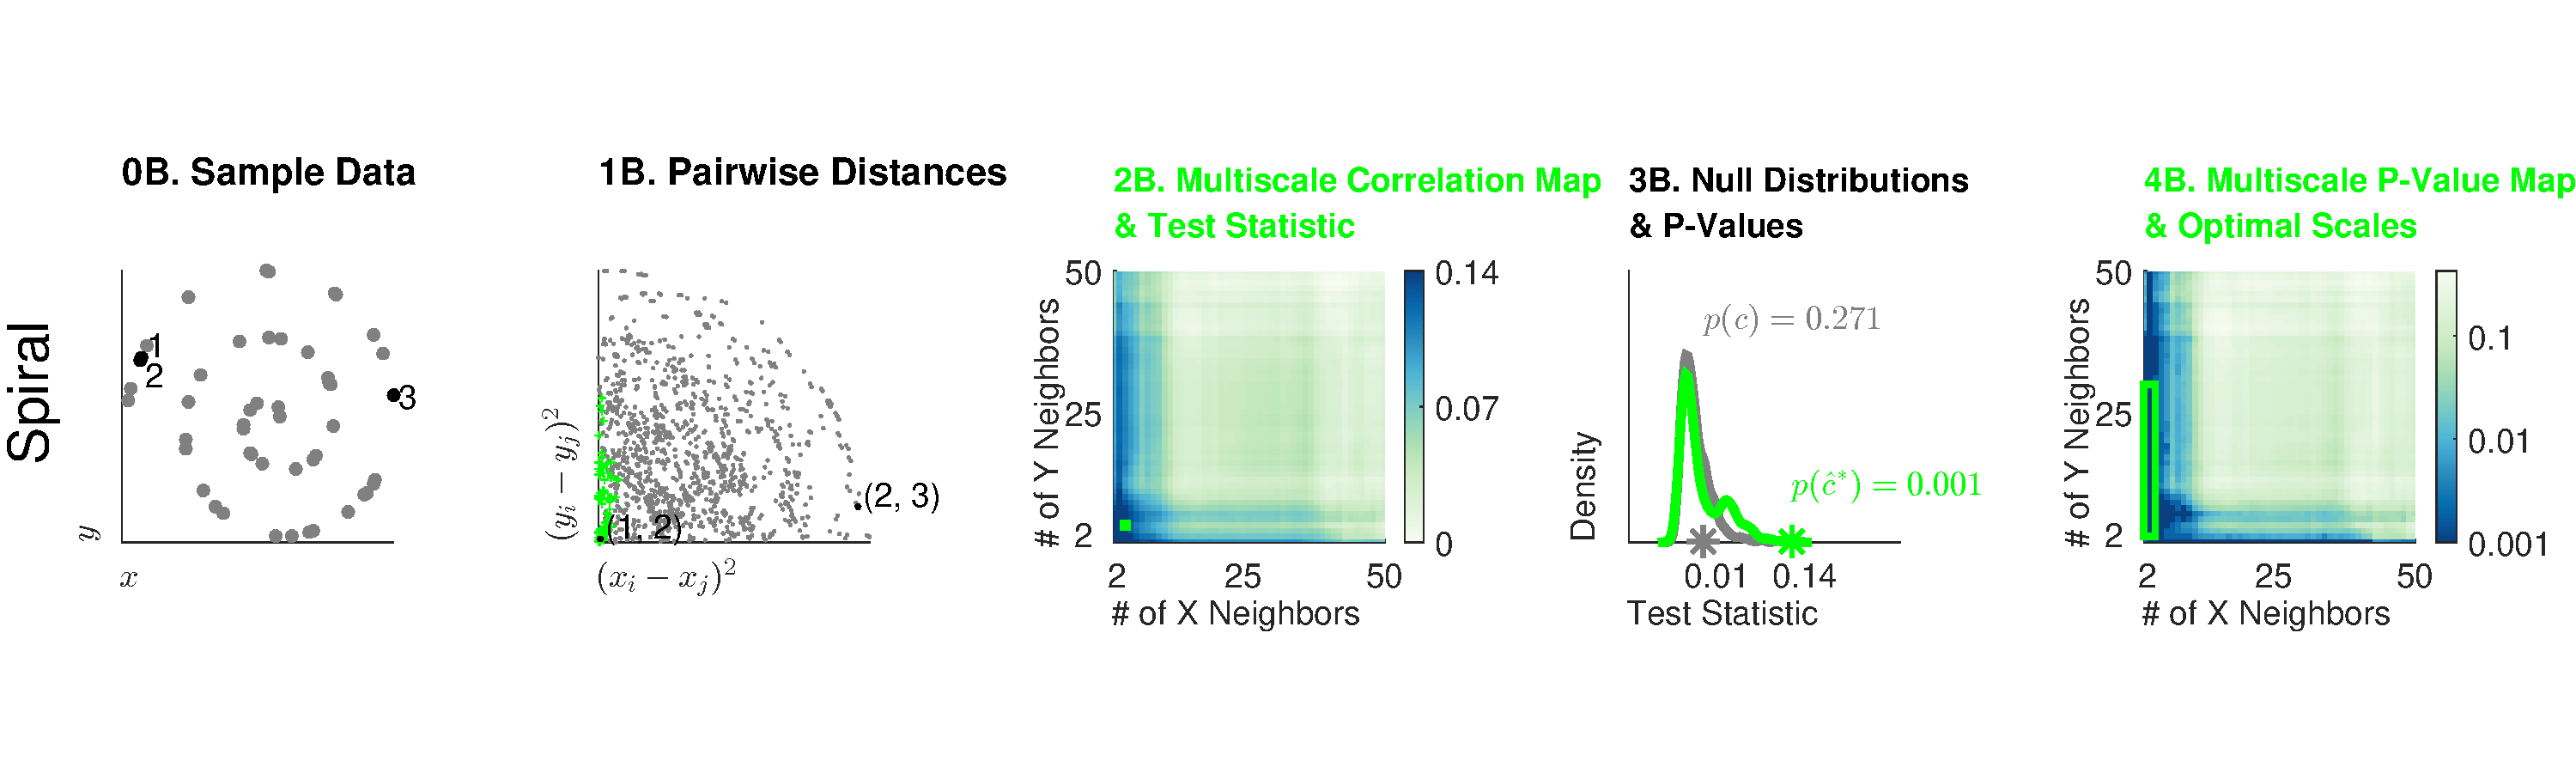
\includegraphics[width=1.0\textwidth,trim={0cm 1.5cm 0cm 5cm},clip]{Figures/Fig8.pdf}
\caption{Illustration of the four steps of Multiscale Generalized Correlation (\Mgc) in two different regions: linear (top) and nonlinear (spiral; bottom). Insights into the data available only from running \Mgc~are highlighted in green.  Results using \Dcorr, an existing state of the art dependence test, are shown for comparative purposes. 
\textbf{(0)}  $50$ pairs of samples of $x$ and $y$ (see Appendix \ref{appen:function} for details). 
Samples $1$, $2$, and $3$ are highlighted to indicate how \Mgc~is able to discover nonlinear relationships. 
% 
\textbf{(1)} Distances are linearly correlated in the linear setting, whereas they are not in the spiral setting.  Green dots are those that \Mgc~uses for its test statistic.
% 
\textbf{(2)} The multiscale correlation map shows the test statistic as the neighborhood size (or scale) increases for both $x$ and $y$, thereby including more distances with which correlation is computed.
The test statistic is increasing as the scales increase for the linear setting, whereas for the spiral setting, only a subset of local scales have large test statistic. The best test statistic is chosen by \Mgc~in both cases, finding the global scale for the linear setting, and a local scale for the spiral setting. Note that previous approaches are all global, and therefore, a special case of \Mgc.
% 
\textbf{(3)} The null distributions are computed via a permutation test. 
 \Mgc~detects significant dependence in both the linear and nonlinear settings, whereas \Dcorr~only detects dependence for the linear setting for this small sample size. 
% 
\textbf{(4)} This is a unique step for \Mgc, which relies on the multiscale p-value map.  \Mgc~estimates the optimal scales. 
For the linear case, many scales, including the global one, are optimal, implying a linear relationship.  On the other hand, for the spiral case, only a small subset of local scales is optimal, implying a strongly nonlinear relationship.
% 
Thus, \Mgc~is able to detect dependence even in highly nonlinear settings with low sample sizes, and reveal the scales of dependence.}
\label{f:newschem}
\end{figure} 

The third step is to compute the p-value via a permutation test, much like previously proposed dependence tests.  The p-value for \Dcorr, $p(c)$, and \Mgc, $p(\hat{c}^*)$, are both highly significant for the linear example. On the other hand, \Dcorr~fails to detect a relationship for the nonlinear setting, where \Mgc~still detects a highly significant relationship.

The fourth step is to find the optimal scales.  This is only possible because \Mgc~computed a multiscale correlation map.  \Mgc~computes the p-value for all scales.  Then, \Mgc~finds the largest rectangle that contains only scales with significant p-values, that is, p-values no more than $p(\hat{c}^*)$. In the linear setting, many scales including the global yield highly significant p-values, implying a nearly linear relationship.  On the other hand, for the non-linear setting, only a set of small local scales yields significant p-values, implying a strongly nonlinear relationship.  

Returning to the first step, we have lighted in green all the pairs that correspond to the optimal scales.  It should be clear that \Mgc~was able to find a linear needle in a nonlinear haystack of data.  This is in contrast to previous approaches.  Perhaps more importantly, rather than merely providing a valid and unbiased p-value, \Mgc~also provides a multiscale map that reveals the nature of the dependence between the two properties of interest, which offers guidance on the type of dependency and further predictive modeling. More mathematical details of \Mgc~are provided in section~\ref{appen:methods}. 
Finally, utilizing \Mgc~is easy and computationally efficient.  Running \Mgc~merely requires inputting $n$ samples of two measured properties.  Our open source implementation\footnote{In both MATLAB and R from our website, \website.} achieves essentially the same computational complexity as previous methods, situating it to be useful in a wide variety of contexts. We therefore further investigate its empirical, computational, and theoretical properties. 





\subsection*{Finite Sample Simulation Experiments}

The first question that we address is: 
when does \Mgc~outperform other approaches, and when does it not?
To answer this question, we compare \Mgc~with four previously proposed state of the art tests: \Mantel, which is widely used in biology and ecology, despite a lack of theoretical support; \Dcorr, as discussed above, \Mcorr, a version of \Dcorr~designed to be unbiased in high-dimensional data \cite{SzekelyRizzo2013a}, and \Hhg~a very impressive test designed for low-dimensional nonlinear settings \cite{HellerGorfine2013}. 
We also compare \Mgc~with ``Oracle \Mgc'', a version of \Mgc~that uses the true distribution of the data to accurately select the optimal scale, rather than estimating it from the data (see section~\ref{appen:mgc2} and Algorithm \ref{alg:power} for details; we refer to data-based \Mgc~as ``Sample'' \Mgc~to avoid confusion).  
We consider $20$ different noisy dependence settings, largely taken from the existing literature, including both nearly linear (1-5), strongly nonlinear (6-19), and independent (20) settings \cite{SzekelyRizzoBakirov2007, SimonTibshirani2012, GorfineHellerHeller2012, HellerGorfine2013, SzekelyRizzo2013a}  
(function details in Supplementary \ref{appen:function}, with a visualization showing both noise-free (black) and noisy (gray) samples in Supplementary Figure~\ref{f:dependencies}).  


To evaluate the different methods, we compute the power of each approach as a function of increasing the dimensionality of $x$.  Power---the probability of rejecting the null when it is  false---is the standard metric for evaluating testing performance for finite samples.  For each setting, we compute the power of each test while increasing dimensionality and effectively decreasing the signal-to-noise ratio.  We compute the average power across dimensions for each setting and algorithm.  
Figure \ref{f:nDSummary} shows that for essentially all 20 settings, and against all other approaches, both \Mgc~and Oracle \Mgc~achieve a higher power.  
Supplementary Figure \ref{f:nDAll} shows the power as a function of dimensionality, rather than the average, which indicates that both \Mgc~and Oracle \Mgc~almost always achieve higher power than the alternative tests for all dimensions, not just the average.  
 Supplementary Figures \ref{f:nDSummary} and \ref{f:1DAll} show similar results,  but keeping the dimensionality of $x$ fixed, while increasing sample size.



\begin{figure}
  \centering
  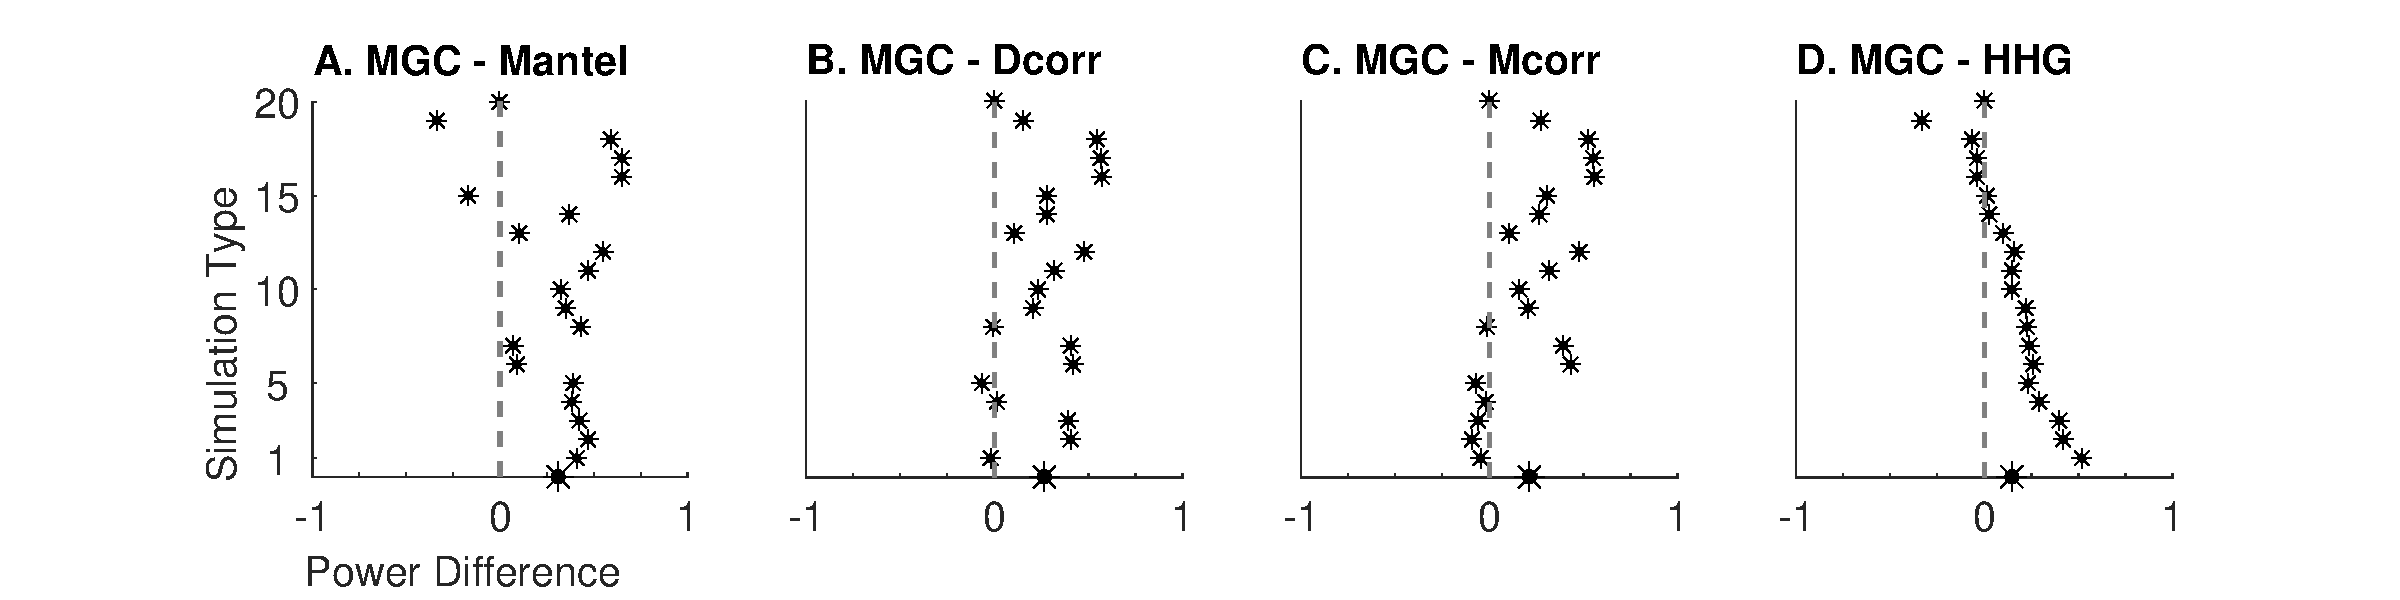
\includegraphics[width=1.0\textwidth,trim={1cm 0 3cm 0},clip]{Figures/FigHDPowerMGCM}
  \caption{Power comparison of both Oracle and Sample \Mgc~to four benchmark dependence tests (denoted $\mathcal{A}$), for the $20$ different settings.  For each setting we compute the average power over a wide range of dimensions $\bar{\beta}$, and plot $\bar{\beta}(\mathcal{A}) - \bar{\beta}(\Mgc)$, for both both Oracle (black dots) and Sample \Mgc~(gray asterisks).  
  The large dots on the x-axis indicate the  power difference averaged over all 20 settings.
\Mgc~nearly dominates existing benchmarks, exhibiting similar or better power for nearly all settings, with Sample \Mgc~being very close to  Oracle \Mgc. 
}
\label{f:nDSummary}
\end{figure}


\subsection*{Discovery of Dependency Across Scales}
\label{main3}

The above sections only demonstrate that \Mgc~provides excellent power, but not that \Mgc~reveals the optimal scales of dependence. 
Figure~\ref{f:powermaps} provides the multiscale power maps for all 20 different high-dimensional scenarios, illustrating how the power of local correlations change with  neighborhood size.
For nearly linear dependencies (1-5), the best neighborhood choice always includes the largest scale, i.e., $k=l=n$. For all strongly nonlinear dependencies (6-19), Oracle \Mgc~chooses smaller scales for $x$ or $y$. Thus a global optimal scale implies a nearly linear dependency, otherwise the dependency is strongly non-linear.
Furthermore, similar dependencies have similar local correlation structure, and thus similar optimal scales. For example, (10) and (11), though very different functions analytically, are qualitatively similar, and yield very similar multiscale power maps.
Similarly,  (12) and (13) are trigonometric functions, and they share a narrow range of significant local correlations.
And both circle (16) and ellipse (17), as well as square (14) and diamond (18), are closely related functions, and have similar multiscale power maps. 
Note that the local structures can be similarly identified by the p-value or test statistic map, and there always exists a large region of local scales that are nearly equally significant in the multiscale maps, which are two important observations that we utilize to design Sample \Mgc.


\begin{figure}[htbp]
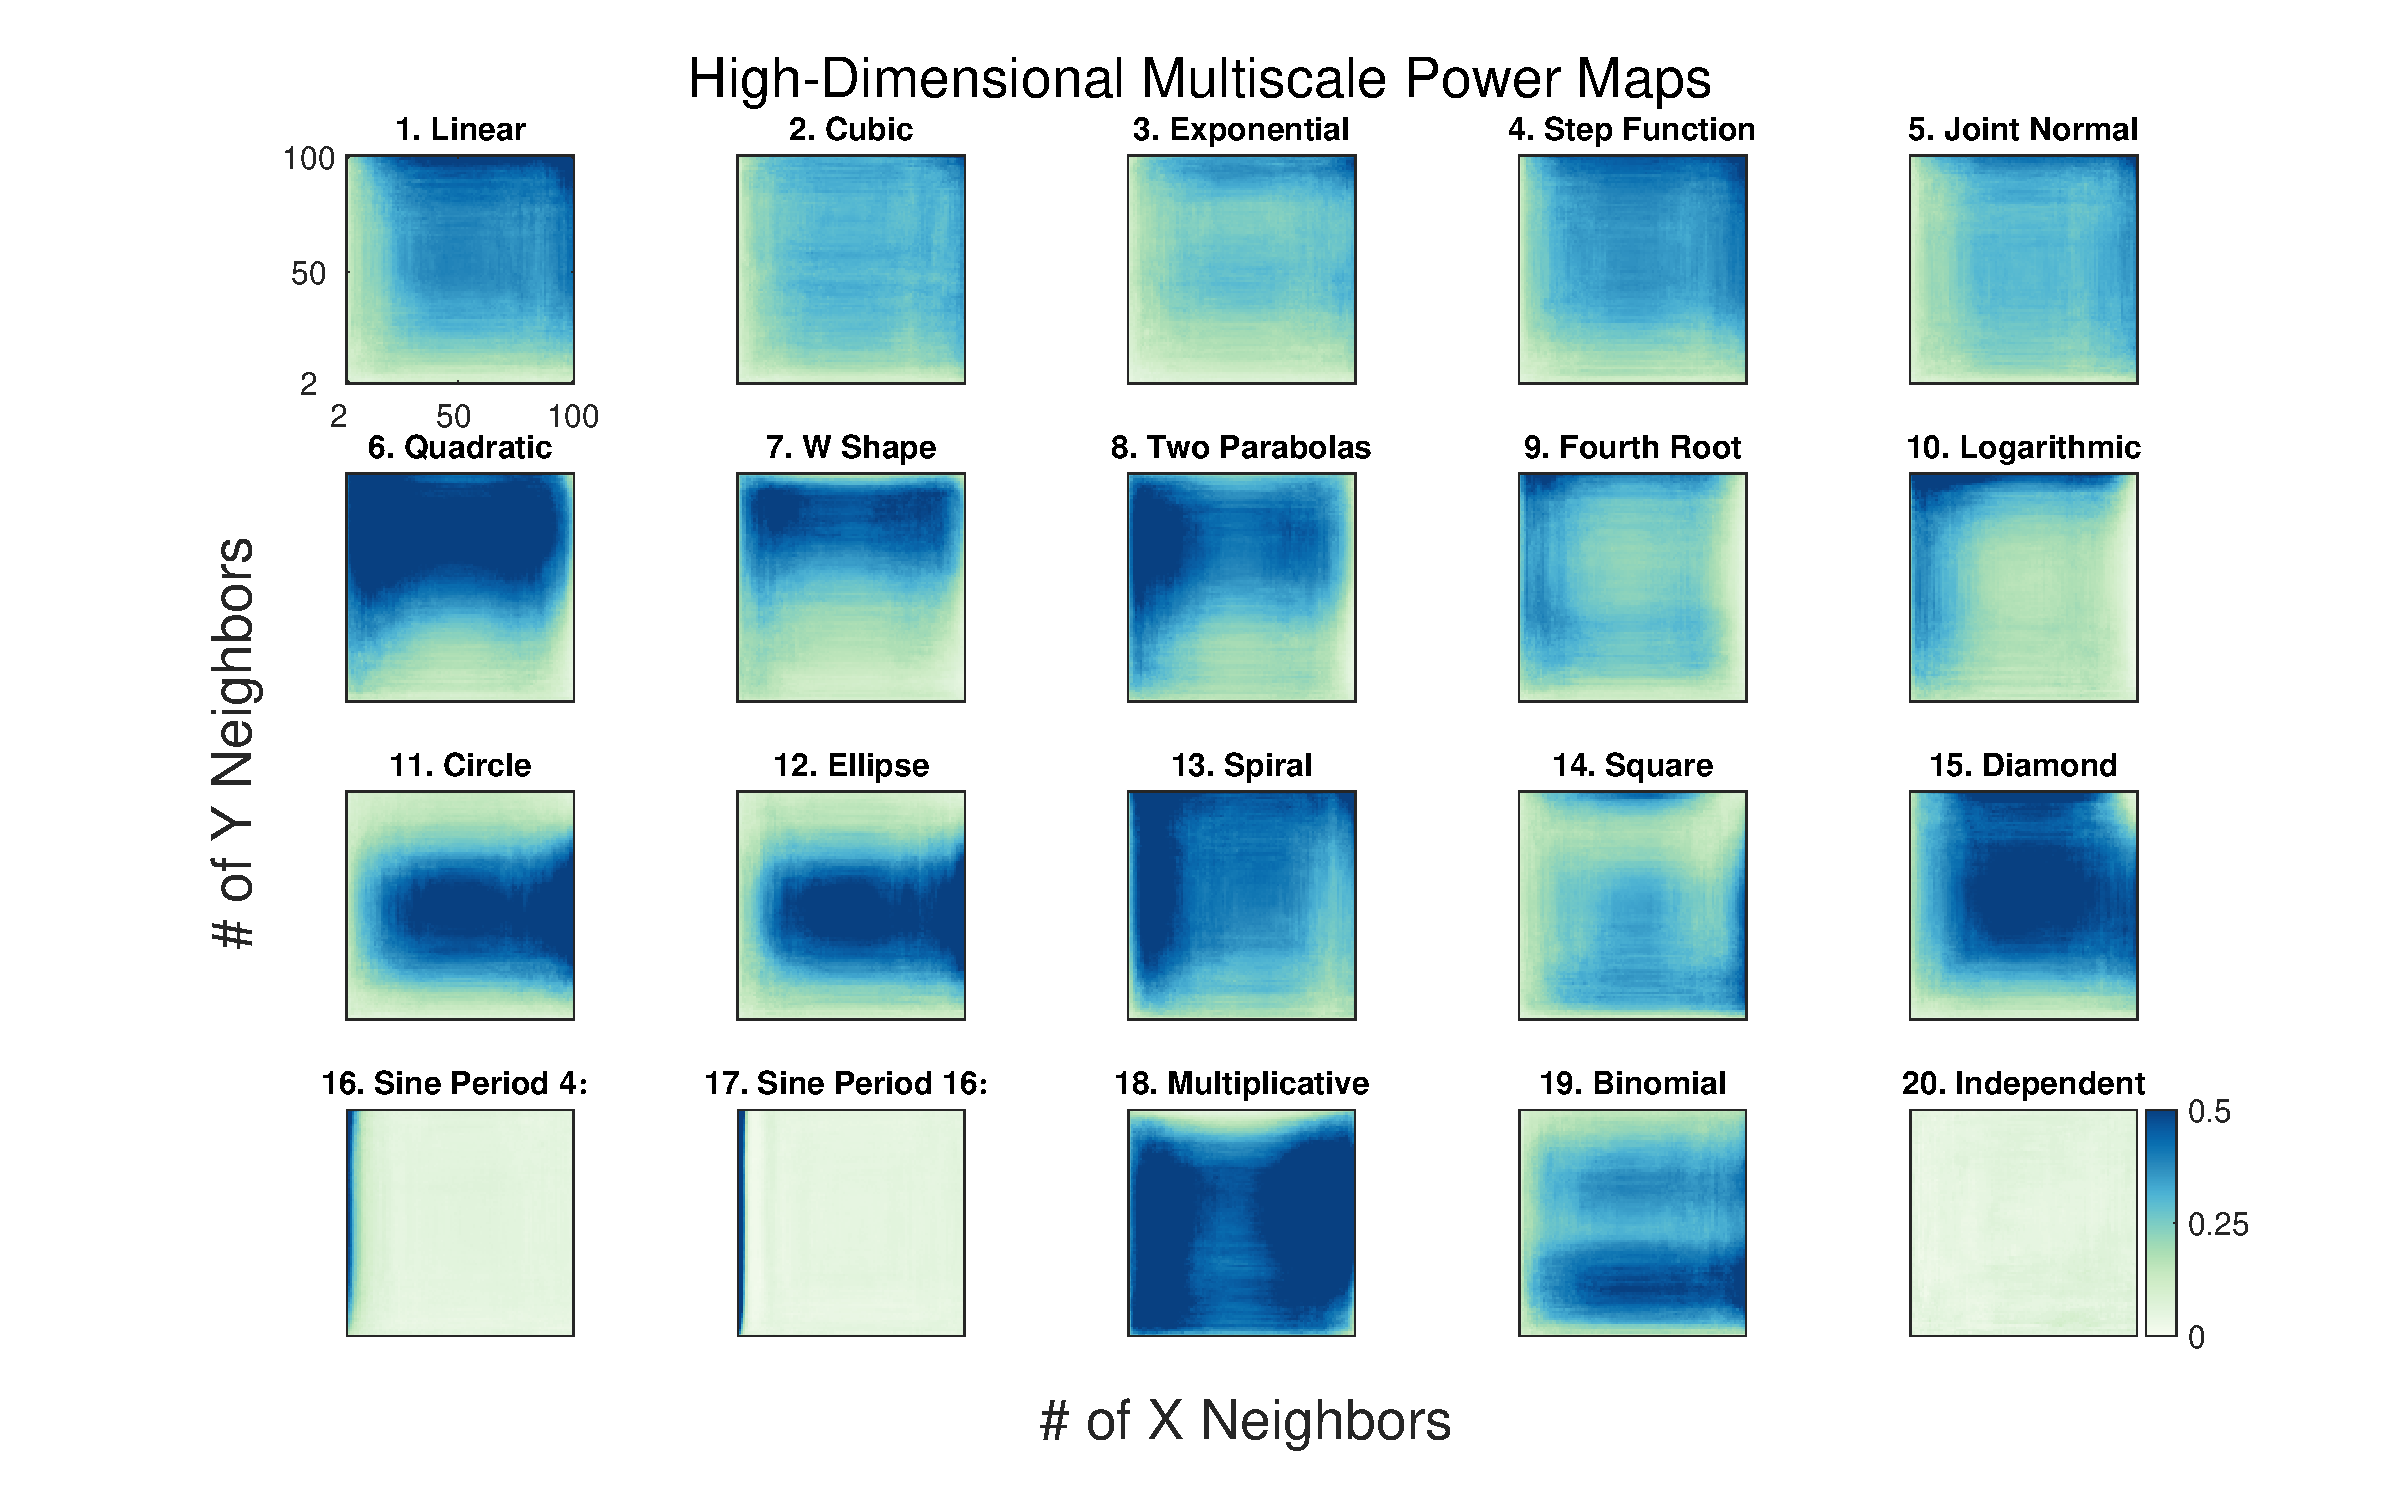
\includegraphics[width=1.0\textwidth,trim={3cm 0.5cm 2.5cm 0.5cm},clip]{Figures/FigHDHeat}
\caption{Multiscale Power Maps reveal the influence of neighborhood size on \Mgc~testing power.
For each of the 20 panels, the abscissa and ordinate denote the number of neighbors for $X$ and  $Y$, respectively. For each simulation, the sample size is $n=100$,  and the dimension is determined by the largest dimension for Oracle \Mgc~to have power exceeding $0.5$ at significance level  $0.05$. Each simulation yields a different multiscale power map, and the global scale is optimal only for nearly linear dependencies, highlighting that \Mgc~not only detects the mere existence of dependency, but also reveals its  structure.}
\label{f:powermaps}
\end{figure}


\subsection*{\Mgc~Theoretically Dominates its Global Counterparts}
\label{s:theory}

The main theoretical result of this manuscript is as follows:
\begin{thm} \label{t:dominate}
Oracle \Mgc~dominates its global correlation counterpart, meaning that \Mgc~is always as good as (in linear settings), and sometimes better than (in nonlinear settings), its corresponding global correlation coefficient, even in finite samples. 
\end{thm}

The above result follows immediately from Theorems \ref{thm1}, \ref{t:linear}, and \ref{t:non}, which are postponed to the Supplementary \ref{appen:theory}.

Therefore, both the simulations and the theorems illustrate that \Mgc~is a consistent test statistic (having power $1$ asymptotically) when it is built on consistent global correlations such as \Dcorr~and \Mcorr~, is equivalent to the global correlation under linear settings, and often yields a much more significant correlation measure and testing power under various nonlinear and high-dimensional settings.
%To our knowledge, this is the first domination theorem in dependence testing, and follows immediately from Theorems \ref{thm1}, \ref{t:linear}, and \ref{t:non}.

\subsection*{Real Data Experiments}
\label{numer3}

In this section, we show how \Mgc~can be applied to various real data of complex structure, as long as proper distance measures can be defined. The resulting correlation and p-value are used for dependence testing, which is able to detect known dependency that previous methods fail to identify. Then the optimal scales further indicate the dependency structure, which aligns with the nature of the data.

A primary goal of statistical analysis and modeling is to suggest the next experiment or analysis. Thus, to further investigate these datasets---for example, to build a brain-based assay for any of the related mental properties---we would start by breaking the data into multiple cohorts, whose sizes correspond to the optimal scales detected here.  Without \Mgc, there would be no dependence test-based justification for any subsequent step.

% \jv{add paragraph here explaining the general results. also stating that we use *all* standard MRI data types to demonstrate the breadth of utility}

\subsubsection*{Brain Activity vs. Personality} 

Our first real data experiment investigates whether there is any dependency between  brain activity and personality.
Adelstein et al. \cite{AdelsteinEtAl2011} were able to detect dependence between certain regions and dimensions of personality, but lacked the tools to test for dependence of the whole brain activity against all five dimensions of personality. 
In this dataset, we have $n=42$ subjects, and for each we obtained  $197$ time-steps of resting-state functional MRI activity, as well as the subject's five-factor personality trait as quantified by  the NEO Personality Inventory-Revised  \cite{Costa1992}. 
The raw brain activity was processed using CPAC \cite{CPAC2015} resulting in $197$ brain regions.
To apply \Mgc, two metrics are required. For the brain activity modality, we ran a spectral analysis on each region, bandpassed and normalized it, and then calculated the Kullback-Leibler divergence across regions to obtain a similarity matrix across all power of regions.  We then used  the normalized Hellinger distance to compute distances between each subject. 
For the five-factor personality data, we  used the Euclidean distance.


Figure \ref{f:real}{\color{magenta}A}  shows that many local scales yield significant p-values ($\approx 0.01$), whereas the global scale fails to detect this significant dependence. In fact, all previously proposed dependence tests under consideration (\Mantel, \Dcorr, \Mcorr, or \Hhg) fail to detect dependence at a significance level of $0.05$, and only \Mgc~provides  insight into the scales of dependence (see Table \ref{t:real}).

\subsubsection*{Brain Shape vs. Disease} 


Our next experiment investigates whether brain shape and disease status are dependent on one another.  Previous investigations have linked major depressive disorder to the hippocampus shape \cite{ParkEtAl2008,PosenerEtAl2003}, though global tests were unable to detect a statistically significant dependence structure at the $\alpha=0.05$ level.
This brain shape versus disease dataset consists of $n=114$ subjects. Each subject has a structural MRI scan as well as a discrete variable indicating whether the subject is clinically depressed $(2)$, high-risk $(1)$, or non-affected $(0)$.  From the MRI data, previous work  extracted both the left and right hippocampi.   For the brain shape modality, they computed the interpoint comparison matrices using a nonlinear landmark matching approach \cite{ParkEtAl2008,BegEtAl2005}. For the  disorder variable, we add white noise bounded by $0.01$ to each label, then form the Euclidean distance (the noise is used to break ties amongst the discrete values and make sure only the diagonal entries of the distance matrix are zero).

Figure \ref{f:real}{\color{magenta}B} provides the p-value map for testing on the right hemisphere using \Mgc. Again, many local scales yield significant p-values, whereas the global scale does not detect a significant dependence  (see Table \ref{t:real}). 

\begin{figure}[htbp]
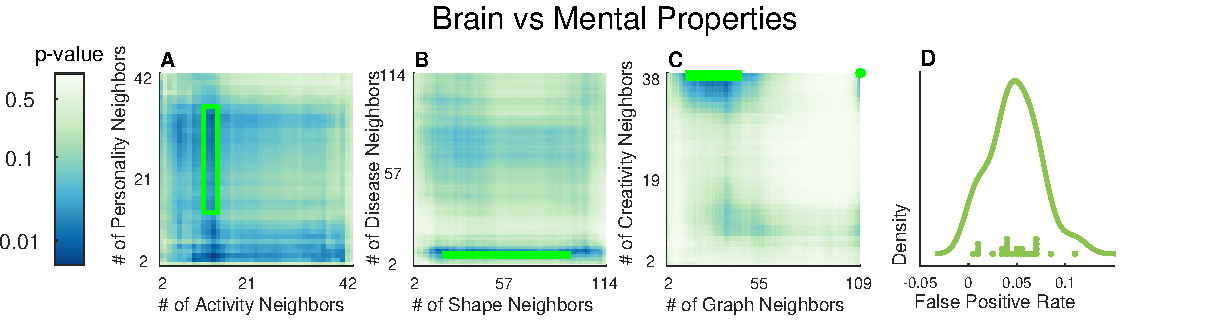
\includegraphics[width=1.0\textwidth,trim={0 0 1.5cm 0},clip]{Figures/FigReal}
\caption{Sample \Mgc~discovers the scales of dependence between various brain and mental properties when they exist, and does not detect dependence when it does not exist.  The left three panels show multiscale p-value maps and their corresponding estimated optimal scales for three different experiments: \textbf{A.}  brain activity vs. five-factor personality model, \textbf{B.}  brain shape vs depressive disease, and \textbf{C.} brain networks vs. creativity. Sample size is $42$, $114$, and $109$, respectively, though the ordinate of these panels only goes as high as the largest possible neighborhood size due to repeated entries.  
For all three, \Mgc~yields significant p-value and reveals the optimal scales of dependence (green rectangles).
\textbf{D.} Density estimate for the false positive rates of Sample \Mgc~on the brain vs synthetic independent noise experiments, with the actual rate of each experiment shown as dots above the x-axis. The mean $\pm$ standard deviation is $0.0538 \pm 0.0394$ respectively, demonstrating that \Mgc~is a valid test and does not inflate the false positives for these real data.}
\label{f:real}
\end{figure}

\begin{table*}[htbp]
\centering
\begin{tabular}{|c||c|c|c|c|c|}
\hline
Testing Pairs / Methods & Sample \Mgc & \Mantel & \Dcorr & \Mcorr & \Hhg \\
\hline
Activity vs Personality & $\textbf{0.033}$  & $0.988$ & $0.647$ & $0.446$ & $0.056$ \\
\hline
Shape vs Disease & $\textbf{0.019}$  & $0.079$ & $0.108$ & $0.106$ & $0.179$ \\
\hline
Network vs Creativity & $\textbf{0.011}$  & $\textbf{0.012}$ & $\textbf{0.011}$ & $\textbf{0.011}$ & $\textbf{0.033}$ \\
\hline
\end{tabular}
\caption{The p-values for real data testing. \Mgc~is the only method that always finds significant relationship and the only method that ever discovers the underlying optimal scale. Bold indicates significant p-value that is $<0.05$.}
\label{t:real}%
\end{table*}

\subsubsection*{Brain Network vs. Creativity}

The next real data experiment investigates whether brain structural networks are independent of creativity.  Neural correlates of creativity have previously been investigated, though largely using structural MRI and cortical thickness \cite{Jung2009}.  Here, we used data from a previously published result on graph similarity \cite{Koutra15a}. For  $n=109$ subjects, we have both diffusion weighted MRI (dMRI) data as well as the subject's ``creativity composite index'' (CCI).  We processed the raw dMRI data via \Migraine, a pipeline for estimating brain networks from diffusion data \cite{GrayRoncal2013}.   
The brain network metric we used was based on  the semi-parametric test statistic \cite{Tang2016} that tests whether pairs of graphs with labeled vertices are sampled from the same distribution.  This test statistic was developed to reduce  the very high dimensionality of adjacency matrices via employing adjacency spectral graph embedding  \cite{Sussman2013}. For these data, we chose to embed each graph into two dimensions for simplicity. We used Euclidean distance to compare CCI values. 



Figure \ref{f:real}{\color{magenta}C} shows that even a global dependence test can ascertain whether the whole brain network is independent of the subject's creativity.  \Mgc~demonstrates that the signal in this case is largely captured by a global relationship, suggesting that there is relatively little to gain by pursuing nonlinear regression techniques. In this setting with high-dimensional and structured data samples and low-sample size, there is no other obvious way that we could effectively determine that the relationship is approximately linear.

%A primary goal of statistical analysis and modeling is to suggest the next experiment or analysis.  For all three of the above investigations, \Mgc~not only found dependence, but also indicated the scales of dependence.  
%Thus, to further investigate these datasets---for example, to build a brain-based assay for any of these mental properties---we would start by breaking the data into multiple cohorts, whose sizes correspond to the optimal scales detected here.  Without \Mgc, there would be no dependence test-based justification for any subsequent step.
\cs{moved above to beginning of real data section}
\cs{add refer to appendix:method}

\subsubsection*{Sample \Mgc~Does Not Inflate False Positive Rates} 


In the final experiment, Sample \Mgc~is applied to test independence between brain voxel activities and a non-existent stimulus, similar to a pair of studies led by Eklund  \cite{EklundKnutsson2012,Eklund2015}. We considered $25$ resting state fMRI data sets from the 1000 functional connectomes project (\url{http://fcon_1000.projects.nitrc.org/}), consisting of a total of $1$,$583$ subjects.
We used CPAC to estimate regional time-series, in particular, using the sequence of pre-processing decisions determined to optimize discriminability \cite{Wang2016}.  The output for each scan is the resting state fMRI time series data containing $200$ regions of interest for $200$ time-steps.
We then also generate an independent stimulus  by sampling from a standard normal distribution at each time step.  Of course, the brain activity data and the stimuli are independent by construction.
For each brain region, we test: ``Is activity of that  brain region independent of the time-varying stimuli?'' We pool brain activity over all of the samples from the population.
Any regions that are detected significant are false positives by definition.  By testing each brain region separately, we obtain a distribution of false positive rates.  If our test is valid, that distribution should be centered around the significance level, which we set at $0.05$ for this experiment.

To conduct this test, we must construct a distance matrix for brain region activity, and another for the stimulus. For each brain region, $g$, we compute the Euclidean distance pairs of time steps,  $\tilde{a}_{ij}^g=\|\mb{x}_{\cdot i}^g-\mb{x}_{\cdot j}^g\|_2$,  where $\mb{x}_{\cdot i}^g$ denotes the population vector of activity of region $g$ at time-step $i$ for all subjects.
For the one-dimensional stimulus, we similarly compute the Euclidean distance between the stimulus values at each pair of time-steps: $\tilde{b}_{ij}= \|y_i - y_j\|_2$.
Note that the distance matrices at different brain regions are distinct, but the stimulus is the same for all brain regions during the same experiment.


For each data set, the above test is carried out for each brain region; the false positive rates of Sample \Mgc~for each dataset are shown in Figure~\ref{f:real}{\color{magenta}D}, which are centered around the critical level $0.05$, as it should be.
In contrast, many standard parametric methods for fMRI analysis, such as generalized linear models, can significantly increase the false positive rates, depending on the data and pre-processing details \cite{EklundKnutsson2012,Eklund2015}. Moreover, even the proposed solutions to those issues make linearity assumptions, thereby limiting detection to only a small subset of possible dependence functions.

\subsection*{Discussion}
\label{conclu}

We propose multiscale generalized correlation (\Mgc) to discover the presence and scales of dependence across disparate properties of data.
We proved that Oracle \Mgc~dominates global approaches in finite samples.  This proof relies on showing first that \Mgc~performs as well as global approaches in certain settings (the linear ones), and then showing that \Mgc~performs \emph{better} than global approaches in other settings (nonlinear ones). 
We further empirically demonstrate via simulations that \Mgc~outperforms global methods regardless of the dimension, sample size, or nonlinearity.  Moreover, in addition to a consistent test, \Mgc~provides a map encoding which scales contain the dependence structure. 
In real data experiments, \Mgc~reveals dependence where global methods fail, discovers the scale of dependence where global methods succeed, and does not falsely detect signals when there are none.


Several other approaches to dependence detection are worth mentioning.
First, a method closely related to distance correlation tests,  is the kernel-based independence test  \cite{GrettonEtAl2005, GrettonGyorfi2010, GrettonEtAl2012}.  Recent work has demonstrated the equivalence between these kernel tests and  energy statistics  \cite{SejdinovicEtAl2013, RamdasEtAl2015}. Thus, we may be able to glean further insights by casting \Mgc~within the kernel framework. Specifically, more efficient tests using asymptotic null distribution approximations for our multiscale tests are possible.
Second,
% 
% \jv{merge in}
% 
However, only a few papers have utilized locality for testing purposes \cite{David1966,Friedman1983,Schilling1986}.  These tests, like the ones based on distance correlation, have the advantage of naturally operating on complicated data, because they only require a comparison function between observations.  They can also have strong theoretical guarantees \cite{Maa1996}, but they are for testing equality of distribution for data from the same modality, and we are interested in testing for dependence across different modalities. 
% 
% \jv{merge this topic in here}
% 
Dumcke et al. \cite{Dumcke2014} recently proposed a related nearest-neighbor based test.  Unfortunately, their proposed test requires estimating relatively high-dimensional densities, and therefore, does not perform particularly well, nor does it have strong theoretical support.
Finally, Reshef et al. \cite{Reshef2011} and Heller et al. \cite{heller2016consistent} are both $1$-dimensional tests, and therefore, not appropriate for our applications (see \cite{SimonTibshirani2012} and \cite{reshef2015empirical} for extensive simulation comparisons demonstrating extensions of their original work).




 \Mgc~can be thought of as a regularized, or sparsified variant of generalized correlation coefficients.  Regularization is central to high-dimensional and ill-posed problems, where dimensionality is larger than sample size.  Thus, it is not surprising that regularizing interpoint comparison matrices yields improved performance.  This connection, however, between dependence testing and regularization is apparently novel.  It opens the door towards considering other regularization techniques for both generalized correlation based dependence testing, and other testing approaches such as \Hhg. In particular, \Hhg~can be thought of as averaging over all scales, rather than regularizing to only consider the optimal ones. The Reshef approach can be thought of similarly.  Therefore, we suspect that this idea could immediately impact other statistical testing frameworks.



There are a number of additional potential extensions of this work.  First, theoretical guidance for choosing the optimal scale for finite samples  in the absence of training data, would be desirable. 
In this work we proved that there exist local scales that improve upon the global scale, and demonstrated that Sample \Mgc~yields tests with power very close to the optimal power, often better than \Hhg~and \Mcorr, and with significant p-values and accurate optimal scale estimation for the real data.  But more theory connecting Oracle \Mgc~and  Sample \Mgc~will yield further insight.


Second, \Mgc~requires a pair of metrics, one for each data type. In this work we selected such metrics using domain knowledge, and mitigated the potential inopportune choice of metric via locality tuning.  If we were able to choose the optimal metric for a given dataset, this would possibly obviate the need for locality, and further improve power. Szekely et al. investigated different norms and exponents to ascertain the impact of different metrics, but was unable to determine optimality.
Metric learning \cite{xing2003distance} addresses learning metrics for different exploitation tasks, so perhaps ideas from that literature can be brought to bear on this problems.  Specifically, perhaps a different one-dimensional family of metrics could yield additional insights into choosing an optimal metric and scale.

Third, essentially all of the tests described in this manuscript are quadratic in sample size.  When sample size gets very large, such a computational burden is intractable.  Recent work from Huo and Szekely  has demonstrated efficient algorithms that are linear in sample size  for one-dimensional data \cite{Huo2016}.  Although it is not clear how to extend the Huo and Szekely approach  to multidimensional data, a subsampling strategy seems viable.  In fact, the multiscale power maps are accurate even when subsampling the data points significantly (not shown), suggesting that subsampling data or pairwise comparisons  could yield an approximate linear time algorithm.  One could also implement \Mgc~using a semi-external computing model \cite{Zheng2016},  which could enable using solid state disk space in a streaming fashion to both speed up computations for big data and enable storing interpoint pairwise comparison matrices larger than what can fit in RAM.

Finally, the notion of multiscale generalized correlations could be used in a wide variety of related exploitation tasks.  In particular, ``energy statistics''---for which $\Dcorr$ and $\Mcorr$ are special cases---have been applied to many different testing scenarios, including goodness-of-fit  \cite{Szekely2005}, analysis of variance  \cite{Rizzo2010}, conditional dependence  \cite{Szekely2014,Wang2015},   and feature selection \cite{LiZhongZhu2012,Zhong2015}.     
In fact, \Mgc~also implements the two-sample (or generally the $K$-sample) test \cite{Szekely2004, heller2016consistent}, and further investigation comparing the advances of \Mgc~to standard methods for two-sample tests is appealing.
Testing independence between graphs and node attributes \cite{Fosdick2015} is another immediate potential application.  And while not previously addressed, using the \Mgc~intuition for dimensionality reduction, classification, and regression seem like very promising future directions, especially because \Mgc~reveals the scales of dependence which can easily be employed in such problems.

To facilitate the reproducibility of this work, as well as myriad applications and extensions, all source code for performing the experiments, generating figures, and the functions themselves are provided in the website, \website, including both R and MATLAB implementations.


\clearpage
\pagestyle{plain}
\bibliographystyle{Science}
\bibliography{MGCbib}


\section*{Acknowledgment}
% \addcontentsline{toc}{section}{Acknowledgment}
This work was partially supported by the
%
National Security Science and Engineering Faculty Fellowship (NSSEFF),
%
the Johns Hopkins University Human Language Technology Center of Excellence (JHU HLT COE),  the
%
Defense Advanced Research Projects Agency's (DARPA) SIMPLEX program through SPAWAR contract N66001-15-C-4041,
%
the XDATA program of DARPA administered through Air Force Research Laboratory contract FA8750-12-2-0303,
%
the Office of Naval Research contract N00014-12-1-0601,
%
the Air Force Office of Scientific Research contract FA955014-1-0033. The authors thank Dr. Brett Mensh of Optimize Science for acting as our intellectual consigliere, and Dr. Ruth Heller for insightful suggestions regarding Sample \Mgc.

\clearpage
\appendix
\setcounter{figure}{0}
\renewcommand\thefigure{S\arabic{figure}}

\section{Global Methods for Testing Dependence}
\label{appen:methods}
To better understand our multiscale generalized correlation, in this section we first establish the statistical framework for testing independence, followed by the notion of the generalized correlation coefficient, and reviewing four existing dependence tests: the \Mantel~test, distance correlation (\Dcorr), modified distance correlation (\Mcorr), and \Hhg. They are arguable the most popular and well-known statistical tests so far, serve as the benchmarks in the main paper, three of which can be used as the global correlation for local correlations and \Mgc.

\subsection{Testing Independence}
To theoretically investigate the performance of any dependence tests requires formalizing the statistical hypotheses.
 
Given pairs of observations $(\mb{x}_{i},\mb{y}_{i}) \in \Real^{D \times D_y}$ for $i=1,\ldots,n$, assume they are independently identically distributed as $(\mbx,\mby)$. If the two random variables \mbx~and \mby~are independent, the joint distribution equals the product of the marginals, i.e., $f_{xy}=f_x f_y$.  Therefore, the common statistical hypotheses for testing independence is as follows:
\begin{align*}
& H_{0}: f_{xy}=f_{x}f_{y},\\
& H_{A}: f_{xy} \neq f_{x}f_{y}.
\end{align*}
Given a test statistic, the testing power equals the probability of rejecting the independence hypothesis when the null hypothesis is false. A test is consistent if and only if the testing power grows to $1$ as sample size increases to infinity under the alternative. 

For testing independence, we would like a test to be universal consistent, i.e., consistent against all possible dependencies, such that it can help discover all types of relationships underlying the given pair of sample data. \Dcorr, \Mcorr, and \Hhg~are consistent against all dependencies with finite second moments, which is almost as good as universal consistent in practice as real data are always finite.

Note that $D$ is the dimension for $\mb{x}$'s, $D_y$ is the dimensionality for $\mb{y}$'s. For all methods below, there is no restriction on the dimensions, e.g., the dimensions can be arbitrarily large, and $D$ is not required to equal $D_y$. The ability to handle data of arbitrary dimension is crucial for modern big data, such that it is important to recognize tests that excel for high-dimensional data. Not all tests do well under high-dimensional dependencies; and there exist some special methods that only operate on 1-dimensional data, such as \cite{Reshef2011}, \cite{heller2016consistent}, \cite{Huo2016}, which are not considered in this paper due to their limited scopes in practice.

\subsection{Generalized Correlation}
Most state-of-art dependence tests operate on distances (or generally, kernels), rather than the sample observations directly. Given pairs of observations $(\mb{x}_{i},\mb{y}_{i}) \in \Real^{D \times D_y}$ for $i=1,\ldots,n$, let $\delta_x$ be the distance function for $\mb{x}$'s and $\delta_y$ for $\mb{y}$'s, one can compute two $n \times n$ distance matrices $\tilde{A}=\{\tilde{a}_{ij}\}$ and $\tilde{B}=\{\tilde{b}_{ij}\}$, where $\tilde{a}_{ij}=\delta_x(\mb{x}_i,\mb{x}_j)$ and $\tilde{b}_{ij}=\delta_y(\mb{y}_i,\mb{y}_j)$. A simple example of the distance function is the Euclidean metric (or $L^{2}$ norm), which is the starting point for all methods here.

Assuming two zero-mean matrices $A$ and $B$ are proper transformations of $\tilde{A}$ and $\tilde{B}$, then a ``generalized correlation coefficient''  \cite{Spearman1904,KendallBook} is written as:
\begin{equation}
\label{generalCoef}
\G(X,Y)= \tfrac{1}{z} {\textstyle \sum_{i,j=1}^n a_{ij} b_{ij}},
\end{equation}
where $z$ is proportional to the standard deviations of $A$ and $B$, that is $z=n^2\sigma_a \sigma_b$. And $X=\{\mb{x}_{1},\cdots, \mb{x}_{n}\} \in \Real^{D \times n}$ and $Y=\{\mb{y}_{1},\cdots, \mb{y}_{n}\} \in \Real^{D_y \times n}$ denote the matrices of sample observations.

In words, $\G$ is the global correlation across \emph{pairwise comparison matrices} $A$ and $B$, rather than the individual data samples. By properly defining $A$ and $B$ based on the distance matrices, the \Mantel~coefficient, \Dcorr, and \Mcorr~can all be written in the form of the generalized correlation coefficient. Note that traditional correlations such as the Pearson's correlation and the rank correlation can also be written by a generalized correlation coefficient, but the $A$ and $B$ in those cases are derived from sample observations rather than the distances; and the \Hhg~test is the only test that cannot be cast into this framework.

For a generalized correlation, it always ranges in $[-1,1]$, has expectation $0$ under independence, implies a stronger dependency when the correlation is further away from $0$, and can serve as the global correlation in implementing \Mgc. To carry out the hypothesis testing on given data by any test statistic, one can conduct a permutation test to obtain the p-value \cite{GoodPermutationBook}, and reject the independent hypothesis when the p-value is lower than the type $1$ error level. 

\subsubsection{The \Mantel~Coefficient}
\label{appen:mantel}
Given the Euclidean distance matrices $\tilde{A}$ and $\tilde{B}$, let $A=\tilde{A}-\bar{a}$ and $B=\tilde{B}-\bar{b}$, where $\bar{a}=\frac{1}{n(n-1)}\sum_{i \neq j}^{n}(a_{ij})$ and similarly for $\bar{b}$.
The \Mantel~coefficient \cite{Mantel1967} is defined as
\begin{equation*}
\Mantel(X,Y)=\frac{\sum_{i \neq j}^{n}a_{ij}b_{ij}}{\sqrt{\sum_{i \neq j}^{n}a_{ij}^2 \sum_{i \neq j}^{n}b_{ij}^2}}.
\end{equation*}
Then the \Mantel~test is carried out by the permutation test.

Unlike distance correlation and \Hhg, the \Mantel~test is not consistent against all dependent alternatives, but it has been a very popular method in biology and ecology, possibly due to its simplicity and effectiveness. One can observe from Figure~\ref{f:1DAll} and ~\ref{f:nDAll} that global \Mantel~is sub-optimal relative to much more recently proposed tests, and appears to be inconsistent for many dependencies. Nonetheless, Oracle \Mgcp~achieves comparable performance to other variants of \Mgc, which implies that \Mgcp~may be consistent with most, if not all dependent alternatives.

\subsubsection{Distance Correlation (\Dcorr)}
\label{appen:dcorr}
Given two distance matrices $\tilde{A}$ and $\tilde{B}$, the sample distance covariance is defined by doubly centering the distance matrices:
\begin{equation*}
\label{dcovEqu}
dcov(X,Y)=\frac{1}{n^2}\sum_{i,j=1}^{n}a_{ij}b_{ij},
\end{equation*}
where $A=H\tilde{A}H$, $B=H\tilde{B}H$, $H=I_{n}-\frac{J_{n}}{n}$, with $I_n$ being the $n \times n$ identity matrix (ones on the diagonal, zeros elsewhere) and $J_n$ being the $n \times n$ matrix of all ones. The sample distance variance is defined as
\begin{align*}
dvar(X) &=\frac{1}{n^2}\sum_{i,j=1}^{n}a_{ij}^{2},\quad dvar(Y) =\frac{1}{n^2}\sum_{i,j=1}^{n}b_{ij}^{2},
\end{align*}
and the sample distance correlation equals
\begin{equation*}
\Dcorr(X,Y)=\frac{dcov(X,Y)}{\sqrt{dvar(X) \cdot dvar(Y)}}.
\end{equation*}

It is shown in \cite{SzekelyRizzoBakirov2007} that as $n \rightarrow \infty$, $\Dcorr(X,Y) \rightarrow \Dcorr(\mb{x},\mb{y}) \geq 0$, where $\Dcorr(\mb{x},\mb{y})$ denotes the population distance correlation between the underlying random variables $\mb{x}$ and $\mb{y}$. The population distance correlation is defined via the characteristic functions of $X$ and $Y$, in such a way that it is zero if and only if $\mb{x}$ and $\mb{y}$ are independent. Thus the sample distance correlation is consistent against all dependencies with finite second moments. All of $dcov, dvar$, and \Dcorr~are always non-negative; and the consistency result holds for a family of metrics not limited to the Euclidean distance \cite{Lyons2013}. Note that the \Dcorr~here equals the square of distance correlation in \cite{SzekelyRizzoBakirov2007}, but for ease of presentation the square naming is dropped here.

Alternatively, calculating the distance covariance by $A=H\tilde{A}$ and $B=\tilde{B}H$ gives the same statistic for distance covariance, i.e., instead of using doubly centered distance matrices, it is equivalent to singly center one distance matrix by row and the other distance matrix by column.
\begin{lem}
The distance covariance $dcov(X,Y)$ is the same under single centering (i.e., $A=H\tilde{A}$ and $B=\tilde{B}H$) and double centering (i.e., $A=H\tilde{A}H$ and $B=H\tilde{B}H$), where $\tilde{A}$ and $\tilde{B}$ are the Euclidean distance matrices of $X$ and $Y$, and $H$ is the centering matrix. 

Moreover, the permutation p-value of global \Dcorr~is the same under single centering and double centering, so is the testing power.
\end{lem}
\begin{proof}
For distance covariance, we can re-write it with matrix traces as follows
\begin{align*}
dcov(X,Y) &= \frac{1}{n^2}\sum_{i,j=1}^{n}a_{ij}b_{ij} \\
 &=\frac{1}{n^2} tr(A\T \times B) \\
 &=\frac{1}{n^2} tr(H\tilde{A}\T HH\tilde{B}H) \\
 &=\frac{1}{n^2} tr(\tilde{A}\T \tilde{B}H) \\
 &=\frac{1}{n^2} tr((H\tilde{A})\T \times (\tilde{B}H)),
\end{align*}
where the second to last equality follows by using the circular property of traces and because $H$ is symmetric and idempotent. Therefore, single centering and double centering yield the same distance covariance.

Although distance variances may not be the same under the two different centering schemes, in the permutation test the distance variances are merely normalization scalars that do not affect the p-value and power, i.e., the test using distance covariance is the same as the test using distance correlation in the permutation test. Therefore the p-value and power of \Dcorr~are also the same under single centering and double centering.
\end{proof}

In Supplementary~\ref{appen:mgc} we will show that \Mgc~based on single-centered \Dcorr~or \Mcorr~is more advantageous than \Mgc~based on double-centered \Dcorr~or\Mcorr, due to rank preserving.

\subsubsection{Modified Distance Correlation (\Mcorr)}
\label{appen:mcorr}
In case of high-dimensional data where the dimension $D$ or $D_y$ increases with the sample size $n$, the sample distance correlation may no longer be appropriate. For example, even for independent Gaussian distributions, $\Dcorr(X,Y) \rightarrow 1$ as $D, D_y \rightarrow \infty$. Therefore \Dcorr~is a biased statistic at large $D$, which not only makes the interpretation and comparison more difficult for distance correlation, but also may severely impair the testing power of \Dcorr~in high-dimensional simulations with limited sample data.

The modified distance correlation is proposed in \cite{SzekelyRizzo2013a} to tackle the bias of sample \Dcorr. Denote the Euclidean distance matrices as $\tilde{A}$ and $\tilde{B}$, and the doubly centered distance matrices as $A'$ and $B'$.  \Mcorr~defines $A$ by modifying the entries of $A'$ by
\[a_{ij} = \left\{
  \begin{array}{lr}
    a'_{ij}-\frac{\tilde{a}_{ij}}{n}, & \mbox{ if } i \neq j, \\
    \frac{1}{n}\sum_{j}\tilde{a}_{ij}-\frac{1}{n^2}\sum_{ij}\tilde{a}_{ij}, &\mbox{ if } i = j,
  \end{array}
\right.
\]
and $B$ modifies the entries of $B'$ similarly.
The modified distance covariance is defined as
\begin{equation*}
mcov(X,Y)=\frac{n}{(n-1)^2(n-3)}\left(\sum_{i \neq j}^{n}a_{ij}b_{ij}-\frac{2}{n-2}\sum_{j=1}^{n}a_{jj}b_{jj}\right),
\end{equation*}
$mvar(X)$ and $mvar(Y)$ are defined similarly.

If $mvar(X) \cdot mvar(Y) \leq 0$, the modified distance correlation is set to $0$ (negativity can only occur when $n\leq 2$, equality can only happen in some special cases); otherwise it is defined as
\begin{equation*}
\Mcorr(X,Y)=\frac{mcov(X,Y)}{\sqrt{mvar(X) \cdot mvar(Y)}}.
\end{equation*}

It is shown in \cite{SzekelyRizzo2013a} that $\Mcorr(X,Y)$ is an unbiased estimator of the population distance correlation $\Dcorr(\mb{x},\mb{y})$ for all $D, D_y, n$; and \Mcorr~is approximately normal even if $D,D_y \rightarrow \infty$. Thus it is always of zero mean under independence, enjoys the same theoretical consistency as \Dcorr, and may work better than \Dcorr~for high-dimensional dependencies.

Similar to the alternative implementation of \Dcorr, we can also use singly centered distance matrices for $A'$ and $B'$ in defining \Mcorr, which does not alter the theoretical advantages of the original \Mcorr. We further set $A_{ii}=B_{ii}=0$ for all $i$, which simplifies the expression of \Mcorr~and is still asymptotically equivalent for testing. Thus we use the single-centered \Mcorr~with zero diagonals for computational expediency and simplicity in the \Mgc~implementation.

\subsubsection{Heller, Heller, \& Gorfine (\Hhg)}
\label{appen:hhg}

The \Hhg~statistic applies Pearson's chi-square test to ranks of distances within each column, and is shown to be better than many global tests including \Dcorr~under common nonlinear dependencies in \cite{GorfineHellerHeller2012, HellerGorfine2013}. Like \Dcorr~and \Mcorr, \Hhg~is distance-based and consistent, but not in the form of the generalized correlation coefficient; and like our \Mgc, it makes use of the rank information, but in a different manner.

Given the Euclidean distance matrices $\tilde{A}=\{\tilde{a}_{ij}\}$ and $\tilde{B}=\{\tilde{b}_{ij}\}$, we denote
\begin{align*}
H_{11}(i,j) &= \sum_{q=1,q\neq i,j}^{n}\mb{I}(\tilde{a}_{iq} \leq \tilde{a}_{ij})\mb{I}(\tilde{b}_{iq} \leq \tilde{b}_{ij}) \\
H_{12}(i,j) &= \sum_{q=1,q\neq i,j}^{n}\mb{I}(\tilde{a}_{iq} \leq \tilde{a}_{ij})\mb{I}(\tilde{b}_{iq} > \tilde{b}_{ij}) \\
H_{21}(i,j) &= \sum_{q=1,q\neq i,j}^{n}\mb{I}(\tilde{a}_{iq} > \tilde{a}_{ij})\mb{I}(\tilde{b}_{iq} \leq \tilde{b}_{ij}) \\
H_{22}(i,j) &= \sum_{q=1,q\neq i,j}^{n}\mb{I}(\tilde{a}_{iq} > \tilde{a}_{ij})\mb{I}(\tilde{b}_{iq} > \tilde{b}_{ij}),
\end{align*}
and the \Hhg~statistic is defined as
\begin{align*}
\Hhg(X,Y) &= \sum_{i=1,j\neq i}^{n} \frac{(n-2)(H_{12}(i,j)H_{21}(i,j)-H_{11}(i,j)H_{22}(i,j))^2}{H_{1 \cdot}(i,j)H_{2 \cdot}(i,j)-H_{\cdot 1}(i,j)H_{\cdot 2}(i,j)},
\end{align*}
where $H_{1 \cdot}=H_{11}+H_{12}$, $H_{2 \cdot}=H_{21}+H_{22}$, $H_{\cdot 1}=H_{11}+H_{21}$, and $H_{\cdot 2}=H_{12}+H_{22}$. Thus \Hhg~is structurally different from all previous distance-based correlations, and cannot be conveniently expressed by Equation~\ref{generalCoef}.

The \Hhg~statistic is consistent in the permutation test. In our numerical simulations, \Hhg~has relatively low power when testing against high-dimensional and noisy linear dependencies, but is often more advantageous than global correlations under nonlinear dependencies, which makes it a strong competitor in general. 
%$\Hhg$ is invariant not only with respect to rescaling of the distances $\delta_x$ and $\delta_y$, but to general monotone transformations.

\section{Multiscale Generalized Correlation (\Mgc)}
\label{appen:mgc}
In this section, we mathematically define the notion of local correlations for any global correlation. The optimal local correlation is chosen as our multilscale generalized correlation, and we distinguish the difference between Oracle and Sample \Mgc~in section~\ref{appen:mgc2}. Theorems characterizing the advantages of \Mgc~are presented in section~\ref{appen:mgc2}. 

Note that the multiscale variants for \Mantel, \Dcorr, and \Mcorr, are denoted as \Mgcp, \Mgcd, and \Mgcm~respectively. Moreover, we always default the notation of \Mgc~to \Mgcm~due to its theoretical and numerical advantages, and our Sample \Mgc~is tailored for \Mgcm~due to the unbiasedness of \Mcorr, with a general Sample \Mgc~strategy for any global correlation presented in section~\ref{appen:mgc2} as well. 

\subsection{Local Correlations}

Despite the consistency of \Dcorr, almost all global correlations struggle in various nonlinear and high-dimensional settings, i.e., the finite sample testing power can be relatively low. We conjectured that their struggles in finite-sample testing were due to the fact that they were \emph{global methods}, which includes all pairs of points in correlation computation. Furthermore, the global correlation cannot provide insight into the scales of the dependence; yet identifying a linear dependency is very important and even an advantage for predicative modeling in practice \cite{cope2009}, comparing to testing all possible dependencies without knowing the underlying relationship. 

To further extend and improve the notion of global correlation, we are motivated by the locality principle, which has reaped considerable benefits in a wide range of data science problems (including classification and regression  \cite{Stone1977}, data compression \cite{DaubechiesWaveletBook}, and recommender systems \cite{Sarwar2000}), and has also become an invaluable tool in nonlinear dimensionality reduction and manifold learning (for example, \cite{
TorgersonBook, 
TenenbaumSilvaLangford2000, 
SaulRoweis2000, 
BelkinNiyogi2003,
DiffusionPNAS,
MMS:NoisyDictionaryLearning}). However, despite many great works, the locality principle is not widely recognized in the statistical community, and often has limited practical values due to its computational inefficiency in many inference tasks.
%However, only a few papers have utilized locality for testing purposes \cite{David1966,Friedman1983,Schilling1986}.  These tests, like the ones based on distance correlation, have the advantage of naturally operating on complicated data, because they only require a comparison function between observations.  They can also have strong theoretical guarantees \cite{Maa1996}, but they are for testing equality of distribution for data from the same modality, and we are interested in testing for dependence across different modalities.

It turns out that the concept of local correlations is very elegant to define, enjoys nice theoretical properties, help detecting the scale of the dependency, and is efficient to implement: let $R(a_{ij})$  be the ``rank'' of $\mb{x}_i$ relative to $\mb{x}_j$, that is, $R(a_{ij})=k$ if $\mb{x}_i$ is the $k^{th}$ closest point (or ``neighbor'') to $\mb{x}_j$, and define $R(b_{ij})$ equivalently for the \mby's. For any neighborhood size $k$ around each $\mb{x}_i$~and any neighborhood size $l$ around each $\mb{y}_i$, we define the local pairwise comparisons:
\begin{equation}
\label{localCoef2}
    \mt{a}_{ij}^k=
    \begin{cases}
      a_{ij}, & \text{if } R(a_{ij}) \leq k, \\    
      0, & \text{otherwise};
    \end{cases} \qquad \qquad
    \mt{b}_{ij}^l=
    \begin{cases}
      b_{ij}, & \text{if } R(b_{ji}) \leq l, \\
      0, & \text{otherwise};
    \end{cases}
\end{equation}
and then let $a^k_{ij}=\mt{a}^k_{ij} - \bar{a}^k$, 
where $\bar{a}^k$ is the local mean. Similarly for $b^l_{ij}$.
The \emph{local} variant of any global generalized correlation coefficient is defined as follows, which effectively excludes large distances:
\begin{equation}
\label{localCoef}
\G^{kl}(X,Y)=\dfrac{1}{z_{kl}} {\textstyle \sum_{i,j=1}^n a_{ij}^k b_{ij}^l},
\end{equation}
where $z_{kl}=n^2 \sigma_a^k \sigma_b^l$,  with $\sigma_a^k$ and $\sigma_b^{l}$ being the standard deviations for the truncated pairwise comparisons. Thus, $c^{kl}$ is the local correlation at a given scale, and the multiscale correlation map can be constructed by computing all local correlations, which allows the discovery of the optimal correlation, i.e., \Mgc. 

Generally, there are a total of $\max(R(a_{ij})) \times \max(R(b_{ij}))$ local correlations, which equals $n^2$ when there exists no repeating values of \mbx~or \mby. We suggest to use minimal ranks in sorting when ties occur, which guarantees that all local correlations are indexed consecutively; alternatively, one may add a very small amount of white noise to break all ties, like in our real data experiment.

For any aforementioned generalized correlation coefficient, its local correlations can be directly implemented as in Equation~\ref{localCoef}, by plugging in the respective $a_{ij}$ and $b_{ij}$ from Equation~\ref{generalCoef}. 

Note that we defined the rank-truncated comparisons differently for $\mt{a}_{ij}^k$ and $\mt{b}_{ij}^l$: $\mt{a}_{ij}^k$ is defined based on ranks within each column, while $\mt{b}_{ij}^l$ is defined based on ranks within each row. By doing so, the ranks are consistent between $\tilde{Z}$ and $Z$ for either $Z=A,B$, and the resulting local correlations are always symmetric even if $A$ and $B$ are not symmetric.

\begin{lem}
\label{lem1}
Each local correlation $\G^{kl}$ is always symmetric regardless of the symmetry of $A$ or $B$. Namely for any $k,l$, 
\begin{align*}
\G^{kl}(X,Y)=\G^{lk}(Y,X).
\end{align*}
Furthermore, the column ranks of $\tilde{A}$ are preserved in $A$ under single centering but not double centering; similarly the row ranks of $\tilde{B}$ are preserved in $B$ under single centering.
\end{lem}
\begin{proof}
For fixed $k,l$, denote $R^{A}$ as the binary matrix such that $R_{A}(i,j)=1$ if $rank(a_{ij}) \leq k$, $R_{A}(i,j)=0$ otherwise. Define $R_{B}$ similarly. Then the rank-truncated pairwise comparisons $\mt{a}_{ij}^k$ and $\mt{b}_{ij}^l$ in Equation~\ref{localCoef2} are the entries of $A \circ R_{A}$ and $B \circ R_{B}\T$ respectively, where $\circ$ denotes the entry-wise product and $\cdot\T$ denotes the matrix transpose.

By the properties of matrix trace, it follows that the local covariance can be rewritten as
\begin{align*}
z_{kl} \G^{kl}(X,Y) &= \textstyle \sum_{i,j=1}^n a_{ij}^k b_{ij}^l \\
 &= tr((A \circ R_{A})\T \times (B \circ R_{B}\T)) \\
 &= tr((B \circ R_{B}\T) \times (A \circ R_{A})\T) \\
 &= tr((B\T \circ R_{B})\T \times (A\T \circ R_{A}\T)).
\end{align*}

When both $A$ and $B$ are symmetric, it is immediate that
\begin{align*}
z_{kl} \G^{kl}(X,Y) &= tr((B\T \circ R_{B})\T \times (A\T \circ R_{A}\T)) \\
 &= tr((B \circ R_{B})\T \times (A \circ R_{A}\T)) \\
 &= z_{lk} \G^{lk}(Y,X),
\end{align*}
such that $\G^{kl}(X,Y)=\G^{lk}(Y,X)$.

Under single centering, however, $A=H \tilde{A}$ and $B=\tilde{B}H$ are no longer symmetric. Nevertheless, the distance matrices $\tilde{A}$ and $\tilde{B}$ are symmetric, so inserting $A\T=\tilde{A}H$ and $B\T=H\tilde{B}$ into the second and fourth equalities above yields
\begin{align*}
z_{kl} \G^{kl}(X,Y) &= tr(((H \tilde{A}) \circ R_{A})\T \times ((\tilde{B}H) \circ R_{B}\T)) \\
 &= tr(((H \tilde{B}) \circ R_{B})\T \times ((\tilde{A}H) \circ R_{A}\T)) \\
 &= z_{lk} \G^{lk}(Y,X),
\end{align*}
so that $\G^{kl}(X,Y)=\G^{lk}(Y,X)$ under single centering.

Therefore each local correlation $\G^{kl}$ is always symmetric for \Dcorr~and \Mcorr,~using either double centering or single centering, and for \Mantel~as well.

As to the rank preservation, the column ranks of the Euclidean distance matrix $\tilde{A}$ are the same as the column ranks of $A=H \tilde{A}$, because $H \tilde{A}$ centers each entry of $\tilde{A}$ by column means, while double centering $H \tilde{A} H$ does not always preserve the original column ranks. Similarly, the row ranks of $\tilde{B}$ are preserved in $B=\tilde{B}H$ but not in $H \tilde{B} H$. Note that the ranks are also preserved in \Mantel.
\end{proof}

Therefore for \Dcorr~and \Mcorr, their local correlations are more faithful in excluding far-away observations that exhibit insignificant dependency, under single centering than under double centering. Therefore, our \Mgcd~and \Mgcm~are based on single centering throughout.

In terms of computational time, the ranking process takes $O(n^2 \log n)$, and computing one local correlation requires $O(n^2)$ (see Algorithm \ref{alg:1scale}). Thus a naive approach to compute all local correlations requires at least $O(n^4)$, and it seems that \Mgc~is just another theoretical tool with formidable computational burden. However, it turns out the multiscale correlation map can be efficiently constructed in $O(n^2)$ by re-using adjacent smaller local correlations to procedurally build all local correlations (see Algorithm \ref{alg:all_scales}), which has essentially the same running time complexity as the global correlation and other benchmarks. Such computational advantage makes \Mgc~a great tool in practice.

\subsection{Oracle and Sample \Mgc}
\label{appen:mgc2}
Among all local correlation, we dub the optimal local correlation as the multiscale generalized correlation. Therefore, \Mgc~can be thought of as a sparse or regularized variant of a global correlation test, and therefore it faces the same dilemma as all regularized algorithms (including sparse methods, feature selection, and dimension reduction): how to efficiently choose the parameters, i.e., the neighborhood choice. By choosing the optimal scale in a principled fashion, \Mgc~both yields a consistent test and reveals the scales of dependence.  

%Many manifold learning algorithms require that the user essentially runs the entire algorithm again from scratch for each different parameter setting, a pursuit that can be exponentially taxing as the number of parameters increases.  
%Since there are $n^2$ different local tests, one for each possible combination of $k$ and $l$, the challenge is to find a way to compute all local tests in a computationally efficient fashion. 

%By noting that the sufficient statistics for larger neighborhood sizes include those for the smaller sizes, one can simply keep track of the sufficient statistics while iteratively increasing neighborhood size, yielding  \emph{all} local correlations in $O(n^2 \log n)$, essentially the same running time complexity as  global correlation coefficients (Algorithms \ref{alg:all_scales}). Specifically, \Mantel, \Dcorr, and \Mcorr~require $O(n^2)$ time, and \Hhg, another state-of-the-art approach,  requires $O(n^2 \log n)$ time \cite{HellerGorfine2013}.  Upon computing the test statistics for all scales, \Mgc~yields ``multiscale maps'', which it then uses to estimate the optimal scale.\footnote{These maps are  related to, but quite distinct from, maps of wavelet coefficients commonly used in geometric counterparts of harmonic analysis \cite{Allard2012,MMS:NoisyDictionaryLearning}.}

Given the distribution, the sample size, and the type $1$ error level, we always define the optimal local correlations (i.e., Oracle \Mgc) as the local correlations that maximize power (the probability of correctly rejecting a false null hypothesis, denote as $\beta$). Mathematically, the optimal scales and Oracle \Mgc~are
\begin{align*}
(k^{*},l^{*}) &=\argmax_{(k,l)}\{\beta(\G_{kl})\}, \\
\G^{*} &=\max\{\G_{k^{*}l^{*}}\} 
\end{align*}
The optimal scales always exist,  are distribution dependent, and are often non-unique. Among all local correlations, it suffices to exclude $\G^{1l}$ and $\G^{k1}$: since $\G^{1l}=\G^{k1}=\G^{11}$, they do not include any neighbor other than each observation itself, merely count the diagonal terms in the distance matrices, and will not be selected as optimal after all. Among all optimal scales, it is equivalent to use any local correlation as the \Mgc~statistic, so we simply take the largest correlation among all optimal scales. 

Therefore, Oracle \Mgc~chooses the optimal scales by simulating from an known or assumed or estimated distribution at a given sample size, and selecting the scales that maximize power, which also yields the multiscale power map for detecting the scale of dependency (Algorithm \ref{alg:power}). Alternatively, if there exists multiple training data, we can select the optimal scales by training data, and compute \Mgc~from the testing data by taking the local correlation at the estimated optimal scale. 

However, in real data testing, often the true distribution is unavailable and hard to estimate, and training data are not available. 
So we cannot utilize the power map to calculate the optimal scales or the optimal test statistic.
To that end, we designed  ``Sample \Mgc'' to estimate Oracle \Mgc, and denote the estimated optimal correlation as $\hat{\G}^{*}$: from the multiscale correlation map, we first threshold out small correlations, then take the largest correlation covering sufficiently many adjacent local correlation as Sample \Mgc; if no such correlation exist, we default $\hat{\G}^{*}$ as the global correlation (Algorithm \ref{alg:sample_mgc}). 

By utilizing the permutation test, we can get the multiscale p-value map for all local correlations, as well as the p-value of \Mgc~(Algorithm \ref{alg:pval}). Note that for Oracle \Mgc, the optimal scales are pre-determined by the power map, and we directly take the local correlation at the optimal scale as the test statistic in the permutation test; while for Sample \Mgc, once we get all the p-values,  the optimal scales are estimated by the tightest bounding box in the p-value map that is no larger than the p-value of sample \Mgc. Because neither the Oracle \Mgc~nor Sample \Mgc~compares multiple statistics, neither suffers from the multiple hypothesis testing problem \cite{Benjamini1995}, and the resulting test is always valid.

The table in Figure \ref{f:schematic} illustrates how \Mgc~is able to detect dependence, even in this spiral example with only $50$ samples, while the global correlation tests fail.  Samples $1$ and $2$ are close to each other in both $x$ and $y$; they therefore contribute to \emph{positive} dependence for all three tests.  However, samples $2$ and $3$ are only close in $x$, not in $y$.  Therefore, in the global tests, \Mantel~and \Mcorr, pair $(2,3)$   \emph{negatively} contributes to dependence testing.  \Mgc~achieves a larger value of the test statistic in this scenario by ignoring  such pairs, thereby achieving a smaller p-value, implying greater power in similar nonlinear settings.  

Note that our Sample \Mgc~algorithm yields $\hat{\G}^{*}$ by identifying significant correlations in the multiscale correlation map, which is tailored for \Mgcm. This is because \Dcorr~is biased, such that its' local correlations are also biased (the expectations may not be $0$ under independence), and significant correlations cannot be easily determined by the the magnitude of each local statistic; while the unbiased-ness of \Mcorr~allows its' local correlations to be compared more meaningfully, and a correlation much larger than $0$ always implies significant local correlation, which allows a fast and valid Sample \Mgc~statistic to be designed for \Mgcm~. 

Still, a general sample estimation technique exists for \Mgcd~and \Mgcp~as well: instead of estimating an optimal correlation within the local correlation map, one may estimate the optimal p-value from the p-value map (e.g., by significant p-values expand along adjacency scales), by treating the estimated p-value as a test statistic and running the permutation test again to compute the true p-value for the sample version of any multiscale variant. This technique is immune to the bias of local correlations, and is suggested by Heller et al. (2016) \cite{heller2016consistent}. Since this general technique requires more random permutations and is much slower, and does not offer any more theoretical or numerical advantages in testing, in this paper we stick to our current Sample \Mgc~method for \Mcorr~only and do not delve into this general technique.

\subsection{Theorems and Proofs of \Mgc}
\label{appen:theory}

Here we prove some useful properties of \Mgc, which shows why it is a more valuable tool than the corresponding global correlation in terms of hypothesis testing and understanding the nature of the relationships.

Let $\G_t$ denote a global generalized correlation coefficient based test statistic, that is, $t$ might indicate \Mantel, \Dcorr, or \Mcorr, and let $\beta_n(\G_t^*)$ denote the power of the corresponding Oracle \Mgc~for $n$ samples; and we drop the subscript when considering asymptotic power.
Recall from the work of Szekely et al. that \Dcorr~and \Mcorr~are both consistent tests, whenever $f_{xy}$ has finite dimension and bounded variance.  Denote the set of distributions satisfying consistency for a given test by $\mc{F}_t$, where $t$ indicates which test we are referring to. Then, we have the following theorem:
\begin{thm}
\label{thm1}
$\beta_n(\G_t^*) \rightarrow 1$ as $n \to \infty$ for all $f_{xy}$ in $\mc{F}_t$.
In words, Oracle \Mgc~is consistent against all dependent alternatives for which its global counterpart is consistent. 
\end{thm}
\begin{proof}
Since $\beta_n(\Mgc_t)=\underset{kl}{\max}\{\beta_n(\G_t^{kl})\}$, for any $f_{xy}$ the power of \Mgc~satisfies
\begin{equation*}
\beta_n(\Mgc_t) \geq \beta_n(\G_t)
\end{equation*}
at any type $1$ error level $\alpha$. So $\beta_n(\Mgc_t) \rightarrow 1$ if $\beta_n(\G_t) \rightarrow 1$.
% 
Therefore $\beta_n(\Mgc_t) \rightarrow 1$ for all $f_{xy}$ in $\mc{F}_t$. In particular, \Mgcd~and \Mgcm~are consistent with all alternatives satisfying certain regularity conditions, because \Dcorr~and \Mcorr~are consistent by \cite{SzekelyRizzoBakirov2007, SzekelyRizzo2013a}. 
\end{proof}

For finite samples, we consider two different kinds of dependencies.
For linear dependencies,  the optimal \Mgc~scale was empirically always the global one (recall Figures~\ref{f:powermaps} and \ref{f:powermaps1}). We therefore conjectured and proved the following:
\begin{thm}
\label{t:linear}
If $\mb{x}$ is linearly dependent on $\mb{y}$, then for any $n$ it always holds that
\begin{equation}
\beta_n(\G_t^*) = \beta_n(\G_t).
\end{equation}
In words, the global scale is the optimal scale for Oracle \Mgc~for linearly dependent data.
\end{thm}
\begin{proof}
To show that \Mgc~is equivalent to the global correlation coefficient, it suffices to show the p-value of $\G^{kl}_t$ is always no less than the p-value of $\G_t$ for all $k,l$ and any $n$ under linear dependence. In the permutation test, the p-value equals the percentage of permutations such that the permuted test statistic is no less than the observed test statistic, so it suffices to compare the number of ``significant'' permutations for $\G_t$ and $\G^{kl}_t$.

Without loss of generality, we assume all of $a_{ij}$, $b_{ij}$, $a_{ij}^{k}$, and $b_{ij}^{l}$ are of zero-mean, as simple centering or not does not affect the p-value; and we assume \Dcorr~with double centering are used, as Lemma~\ref{lem1} shows that double centering and simple centering yield the same testing power and p-value.

Under linear dependency, by Cauchy-Schwarz inequality the distance correlation satisfies
\begin{align*}
& dcov(X,Y) = \sqrt{dvar(X) \cdot dvar(Y)} \quad\Rightarrow\quad 1=\G(X, Y) \geq \G(X, Y_{\pi})
\end{align*}
for any permutation $\pi$, where the equality holds if and only if $X$ is a scalar multiple of $Y_{\pi}$, i.e., $a_{ij}=b_{\pi^{-1}(i) \pi^{-1}(j)}$ for all $i,j$, where $\pi^{-1}(\cdot)$ denotes the inverse permutation. 

Thus for the global correlation, there only exist permutations such that the permuted test statistic equals the observed test statistic. However, for all those ``significant'' permutations for $\G$, they are also ``significant'' for each $\G^{kl}$, i.e., $a_{ij}^{k}=b_{\pi^{-1}(i) \pi^{-1}(j)}^{l}$ if $a_{ij}=b_{\pi^{-1}(i) \pi^{-1}(j)}$, such that $\G^{kl}(X, Y)=\G^{kl}(X, Y_{\pi})$; and there may exist other ``significant'' permutations such that $\G^{kl}(X, Y) \leq \G^{kl}(X, Y_{\pi})$.

Therefore the number of ``significant'' permutations for $\G^{kl}$ at least equals those for $\G$ under linear dependency, and the p-value of $\G^{kl}$ cannot be less than the p-value of $\G$, in which case the global correlation is optimal for \Mgc. 
\end{proof}

Under nonlinear dependencies and finite sample sizes (which characterizes essentially all real data), we noted that \Mgc~typically achieved better power than its corresponding global correlation. 
We therefore conjectured and proved the following:
\begin{thm}
\label{t:non}
There exists $f_{xy}$ and $n$ such that
\begin{equation}
\beta_n(\G_t^*) \geq \beta_n(\G^{k,l}_{t}) > \beta_n(\G_{t}).
\end{equation}
In words, for finite samples, many different scales of \Mgc~can be better than the global scale under certain nonlinear dependency.
\end{thm}
\begin{proof}
We give a simple discrete example of $f_{xy}$ at $n=7$, such that the p-value of \Mgcm~is strictly lower than the p-value of \Mcorr.

Suppose under the alternative, each pair of observation $(\mb{x},\mb{y})$ is sampled as follows:
\begin{align*}
\mb{x} &\in \left\{-1,-\frac{2}{3},-\frac{1}{3},0,\frac{1}{3},\frac{2}{3},1\right\} \mbox{ without replacement}, \\
\mb{y} &= \mb{x}^2,
\end{align*}
which is a discrete version of the quadratic relationship in the simulations.

At $n=7$, we can directly calculate $\G^{kl}(X, Y)$ and $\{\G^{kl}(X, YQ)\}$ for all permutation matrices $Q$. It follows that the p-value of \Mcorr~is $\frac{151}{210} \approx 0.72$, while $\G^{kl}(X, Y)=\frac{29}{126} \approx 0.23$ at $(k,l)=(2,4)$. Note that in this case, $k$ is bounded above by $n=7$ while $l$ is bounded above by $4$ due to the repeating points in $Y$. 

Then by choosing $\alpha=0.24$, \Mgc~has power unity while global \Mcorr~has power $0$, i.e., \Mgc~successfully identifies the dependency in this example while global \Mcorr~fails.

Note that we can always consider sample points in $[-1,1]$ for $X$, increase $n$ and reach the same conclusion with more significant p-values; but the computation of all possible permuted test statistics becomes more time-consuming as $n$ increases. The same conclusion also holds for \Mgcd~and \Mgcp~using the same example.
\end{proof}
Note that Theorem~\ref{t:linear} and Theorem~\ref{t:non} hold for any of the \Mgc~varieties, including  \Dcorr, \Mcorr, and \Mantel.

The proof of Theorem~\ref{t:linear} is straightforward.  The proof of Theorem~\ref{t:non} is a constructive one. More specifically, we constructed a quadratic function and sampled data a finite number of times and computed the exact p-value for both \Mgc~and \Dcorr, proving that \Mgc~has higher power in this setting. This shows that \Mgc~can outperform its global counterpart even for the most modestly nonlinear functions.  Because any function can be approximated by a polynomial expansion \cite{RudinBook}, the proof of Theorem~\ref{t:non} suggests that \Mgc~is able to outperform its corresponding global correlation on a wide variety of nonlinear functions, which is indeed the case throughout the numerical simulations. 

Taken together, the three theorems above lead to the main theorem~\ref{t:dominate} in the main paper.

\section{Simulation Functions}
\label{appen:function}

This section provides the $20$ different dependency functions used in the simulations.  We used essentially the exact same settings as previous publications to ensure a fair comparison \cite{SzekelyRizzoBakirov2007, SimonTibshirani2012, SimonTibshirani2012, GorfineHellerHeller2012}.  We only made changes to add white noise, and a weight vector for higher dimensions, thereby making them more difficult, to better compare all methods throughout different dimensions and sample sizes. We also included a few additional settings.

For each sample $\mb{x} \in \Real^{D}$, we denote $\mb{x}_{[d]}, d=1,\ldots,D$ as the $d^{th}$ dimension of the vector \mbx. For the purpose of high-dimensional simulations, $w \in \Real^{D}$ is a decaying vector with $w_{[d]}=1/d$ for each $d$, such that $w\T \mb{x}$ is a 
% one-dimensional 
weighted summation of all dimensions of \mbx. %, which equals \mb{x}~if $D=1$.
Furthermore, $\mc{U}(a,b)$ denotes the uniform distribution on the interval $(a,b)$, $\mc{B}(p)$ denotes the Bernoulli distribution with probability $p$, $\mc{N}(\mu,{\Sigma})$ denotes the normal distribution with mean ${\mu}$ and covariance ${\Sigma}$, 
$u$ and $v$ represent realizations from some auxiliary random variables, $c$ is a scalar constant to control the noise level (which equals $1$ for one-dimensional simulations and $0$ otherwise), and $\epsilon$ is sampled from an independent standard normal distribution unless mentioned otherwise.

For all of the below equations, $(\mb{x},\mb{y}) \overset{iid}{\sim} f_{xy} = f_{y|x} f_x$. For each setting, we provide the space of $(\mb{x},\mb{y})$, and define $f_{y|x}$ and $f_x$, as well as any additional auxiliary distributions.

\setcounter{equation}{0}
\begin{compactenum}
\item Linear $(\mb{x},\mb{y}) \in \Real^{D} \times \Real$,
\begin{align*}
\mb{x} &\sim \mc{U}(-1,1)^{D},\\
\mb{y} &=w\T \mb{x}+c\epsilon.
\end{align*}
\item Exponential $(\mb{x},\mb{y}) \in \Real^{D} \times \Real$:
\begin{align*}
\mb{x} &\sim \mc{U}(0,3)^{D}, \\
\mb{y} &=exp(w\T \mb{x})+10c\epsilon.
\end{align*}
\item Cubic $(\mb{x},\mb{y}) \in \Real^{D} \times \Real$:
\begin{align*}
\mb{x} &\sim \mc{U}(-1,1)^{D}, \\
\mb{y} &=128(w\T \mb{x}-\tfrac{1}{3})^3+48(w\T \mb{x}-\tfrac{1}{3})^2-12(w\T \mb{x}-\tfrac{1}{3})+80c\epsilon.
\end{align*}
\item Joint normal $(\mb{x},\mb{y}) \in \Real^{D} \times \Real^{D}$: Let $\rho=1/2D$, $I_{D}$ be the identity matrix of size $D \times D$, $J_{D}$ be the matrix of ones of size $D \times D$, and $\Sigma = \begin{bmatrix} I_{D}&\rho J_{D}\\ \rho J_{D}& (1+0.5c) I_{D} \end{bmatrix}$. Then let $\epsilon \sim \mc{N}(0, I_{D})$,
\begin{align*}
(\mb{x}, \mb{y}) &\sim \mc{N}(0, \Sigma). 
\end{align*}
\item Step Function $(\mb{x},\mb{y}) \in \Real^{D} \times \Real$:
\begin{align*}
\mb{x} &\sim \mc{U}(-1,1)^{D},\\
\mb{y} &=\mb{I}(w\T \mb{x}>0)+\epsilon,
\end{align*}
where $\mb{I}$ is the indicator function, that is $\mb{I}(z)$ is unity whenever $z$ true, and zero otherwise.
\item Quadratic $(\mb{x},\mb{y}) \in \Real^{D} \times \Real$:
\begin{align*}
\mb{x} &\sim \mc{U}(-1,1)^{D},\\
\mb{y}&=(w\T \mb{x})^2+0.5c\epsilon.
\end{align*}
\item W Shape $(\mb{x},\mb{y}) \in \Real^{D} \times \Real$:  $u \sim \mc{U}(-1,1)^{D}$,
\begin{align*}
\mb{x} &\sim \mc{U}(-1,1)^{D},\\
\mb{y}&=4\left[ \left( (w\T \mb{x})^2 - \tfrac{1}{2} \right)^2 + w\T u/500 \right]+0.5c\epsilon.
\end{align*}
\item Spiral $(\mb{x},\mb{y}) \in \Real^{D} \times \Real$: $u \sim \mc{U}(0,5)$, $\epsilon \sim \mc{N}(0, 1)$,
\begin{align*}
\mb{x}_{[d]}&=u \sin(\pi u)  \cos^{d}(\pi u) \mbox{ for $d=1,\ldots,D-1$},\\
\mb{x}_{[D]}&=u \cos^{D}(\pi u),\\
\mb{y}&= u \sin(\pi u) +0.4 D\epsilon.
\end{align*}
\item Uncorrelated Bernoulli $(\mb{x},\mb{y}) \in \Real^{D} \times \Real$: $u \sim \mc{B}(0.5)$, $\epsilon_{1} \sim \mc{N}(0, I_{D})$, $\epsilon_{2} \sim \mc{N}(0, 1)$,
\begin{align*}
\mb{x} &\sim \mc{B}(0.5)^{D}+0.5\epsilon_{1},\\
\mb{y}&=(2u-1)w\T \mb{x}+0.5\epsilon_{2}.
\end{align*}
\item Logarithmic $(\mb{x},\mb{y}) \in \Real^{D} \times \Real^{D}$: $\epsilon \sim \mc{N}(0, I_{D})$
\begin{align*}
\mb{x} &\sim \mc{N}(0, I_{D}),\\
\mb{y}_{[d]}&=2\log_{2}(\mb{x}_{[d]})+3c\epsilon_{[d]},
\end{align*}
for $d=1,\ldots,D$.
\item Fourth Root $(\mb{x},\mb{y}) \in \Real^{D} \times \Real$:
\begin{align*}
\mb{x} &\sim \mc{U}(-1,1)^{D},\\
\mb{y}&=|w\T \mb{x}|^\frac{1}{4}+\frac{c}{4}\epsilon.
\end{align*}
\item Sine Period $4\pi$ $(\mb{x},\mb{y}) \in \Real^{D} \times \Real$: $u \sim \mc{U}(-1,1)$, $v \sim \mc{N}(0,1)^{D}$, $\theta=4\pi$,
\begin{align*}
\mb{x}_{[d]}&=u+0.02 D v_{[d]} \mbox{ for $d=1,\ldots,D$}, \\
\mb{y}&=\sin ( \theta x )+c\epsilon.
\end{align*}
\item Sine Period $16\pi$ $(\mb{x},\mb{y}) \in \Real^{D} \times \Real$: Same as above except $\theta=16\pi$ and the noise on $\mb{y}$ is changed to $0.5c\epsilon$.
\item Square $(\mb{x},\mb{y}) \in \Real^{D} \times \Real^{D}$: Let $u \sim \mc{U}(-1,1)$, $v \sim \mc{U}(-1,1)$, $\epsilon \sim \mc{N}(0,1)^{D}$, $\theta=-\frac{\pi}{8}$. Then
\begin{align*}
\mb{x}_{[d]}&=u \cos\theta + v \sin\theta + 0.05 D\epsilon_{[d]},\\
\mb{y}_{[d]}&=-u \sin\theta + v \cos\theta,
\end{align*}
for $d=1,\ldots,D$.
\item Two Parabolas $(\mb{x},\mb{y}) \in \Real^{D} \times \Real$: $\epsilon \sim \mc{U}(0,1)$, $u \sim \mc{B}(0.5)$,
\begin{align*}
\mb{x} &\sim \mc{U}(-1,1)^{D},\\
\mb{y}&=\left( (w\T \mb{x})^2  + 2c\epsilon\right) \cdot (u-\tfrac{1}{2}).
\end{align*}
\item Circle $(\mb{x},\mb{y}) \in \Real^{D} \times \Real$: $u \sim \mc{U}(-1,1)^{D}$, $\epsilon \sim \mc{N}(0, I_{D})$, $r=1$,
\begin{align*}
\mb{x}_{[d]}&=r \left(\sin(\pi u_{[d+1]})  \prod_{j=1}^{d} \cos(\pi u_{[j]})+0.4 \epsilon_{[d]}\right) \mbox{ for $d=1,\ldots,D-1$},\\
\mb{x}_{[D]}&=r \left(\prod_{j=1}^{D} \cos(\pi u_{[j]})+0.4 \epsilon_{[D]}\right),\\
\mb{y}&= \sin(\pi u_{[1]}).
\end{align*}
\item Ellipse $(\mb{x},\mb{y}) \in \Real^{D} \times \Real$: Same as above except $r=5$.
\item Diamond $(\mb{x},\mb{y}) \in \Real^{D} \times \Real^{D}$: Same as (8) Square except $\theta=-\frac{\pi}{4}$.
\item Multiplicative Noise $(\mb{x},\mb{y}) \in \Real^{D} \times \Real^{D}$: $u \sim \mc{N}(0, I_{D})$, 
\begin{align*}
\mb{x} &\sim \mc{N}(0, I_{D}),\\
\mb{y}_{[d]}&=u_{[d]}\mb{x}_{[d]},
\end{align*}
for $d=1,\ldots,D$.
\item Independent Clouds $(\mb{x},\mb{y}) \in \Real^{D} \times \Real^{D}$: Let $u \sim \mc{N}(0,I_{D})$, $v \sim \mc{N}(0,I_{D})$, $u' \sim \mc{B}(0.5)^{D}$, $v' \sim \mc{B}(0.5)^{D}$. Then
\begin{align*}
\mb{x}&=u/3+2u'-1,\\
\mb{y}&=v/3+2v'-1.
\end{align*}
\end{compactenum}

For each distribution, $\mb{x}$ and $\mb{y}$ are dependent except  (20); for some settings (8,14,16-18) they are conditionally independent upon conditioning on the respective auxiliary variables, while for others they are
 ``directly'' dependent. 
% Given $(\mb{x}_{i},\mb{y}_{i})$ pairs for $i=1,\ldots,n$, set $X=\{\mb{x}_{1},\cdots, \mb{x}_{n}\} \in \Real^{D \times n}$ and $Y=\{\mb{y}_{1},\cdots, \mb{y}_{n}\} \in \Real^{D_y \times n}$, where $D_y$ is the dimensionality of \mby. 
A visualization of each dependency with $D=D_y=1$ is shown in Figure~\ref{f:dependencies}.


For the increasing dimension simulation in the main paper, we always set $c=0$ and $n=100$, with $D$ increasing.  For types  $4,10,14,18,19,20$, we let $D_y=D$; otherwise, we let $D_y=1$. 
The decaying vector $w$ is utilized for $D>1$ to make the high-dimensional settings more difficult (otherwise, additional dimensions only add more signal).


\section{Supplementary Figures}
\label{appen:figs}

\begin{figure}[htbp]
\vspace{-50pt}
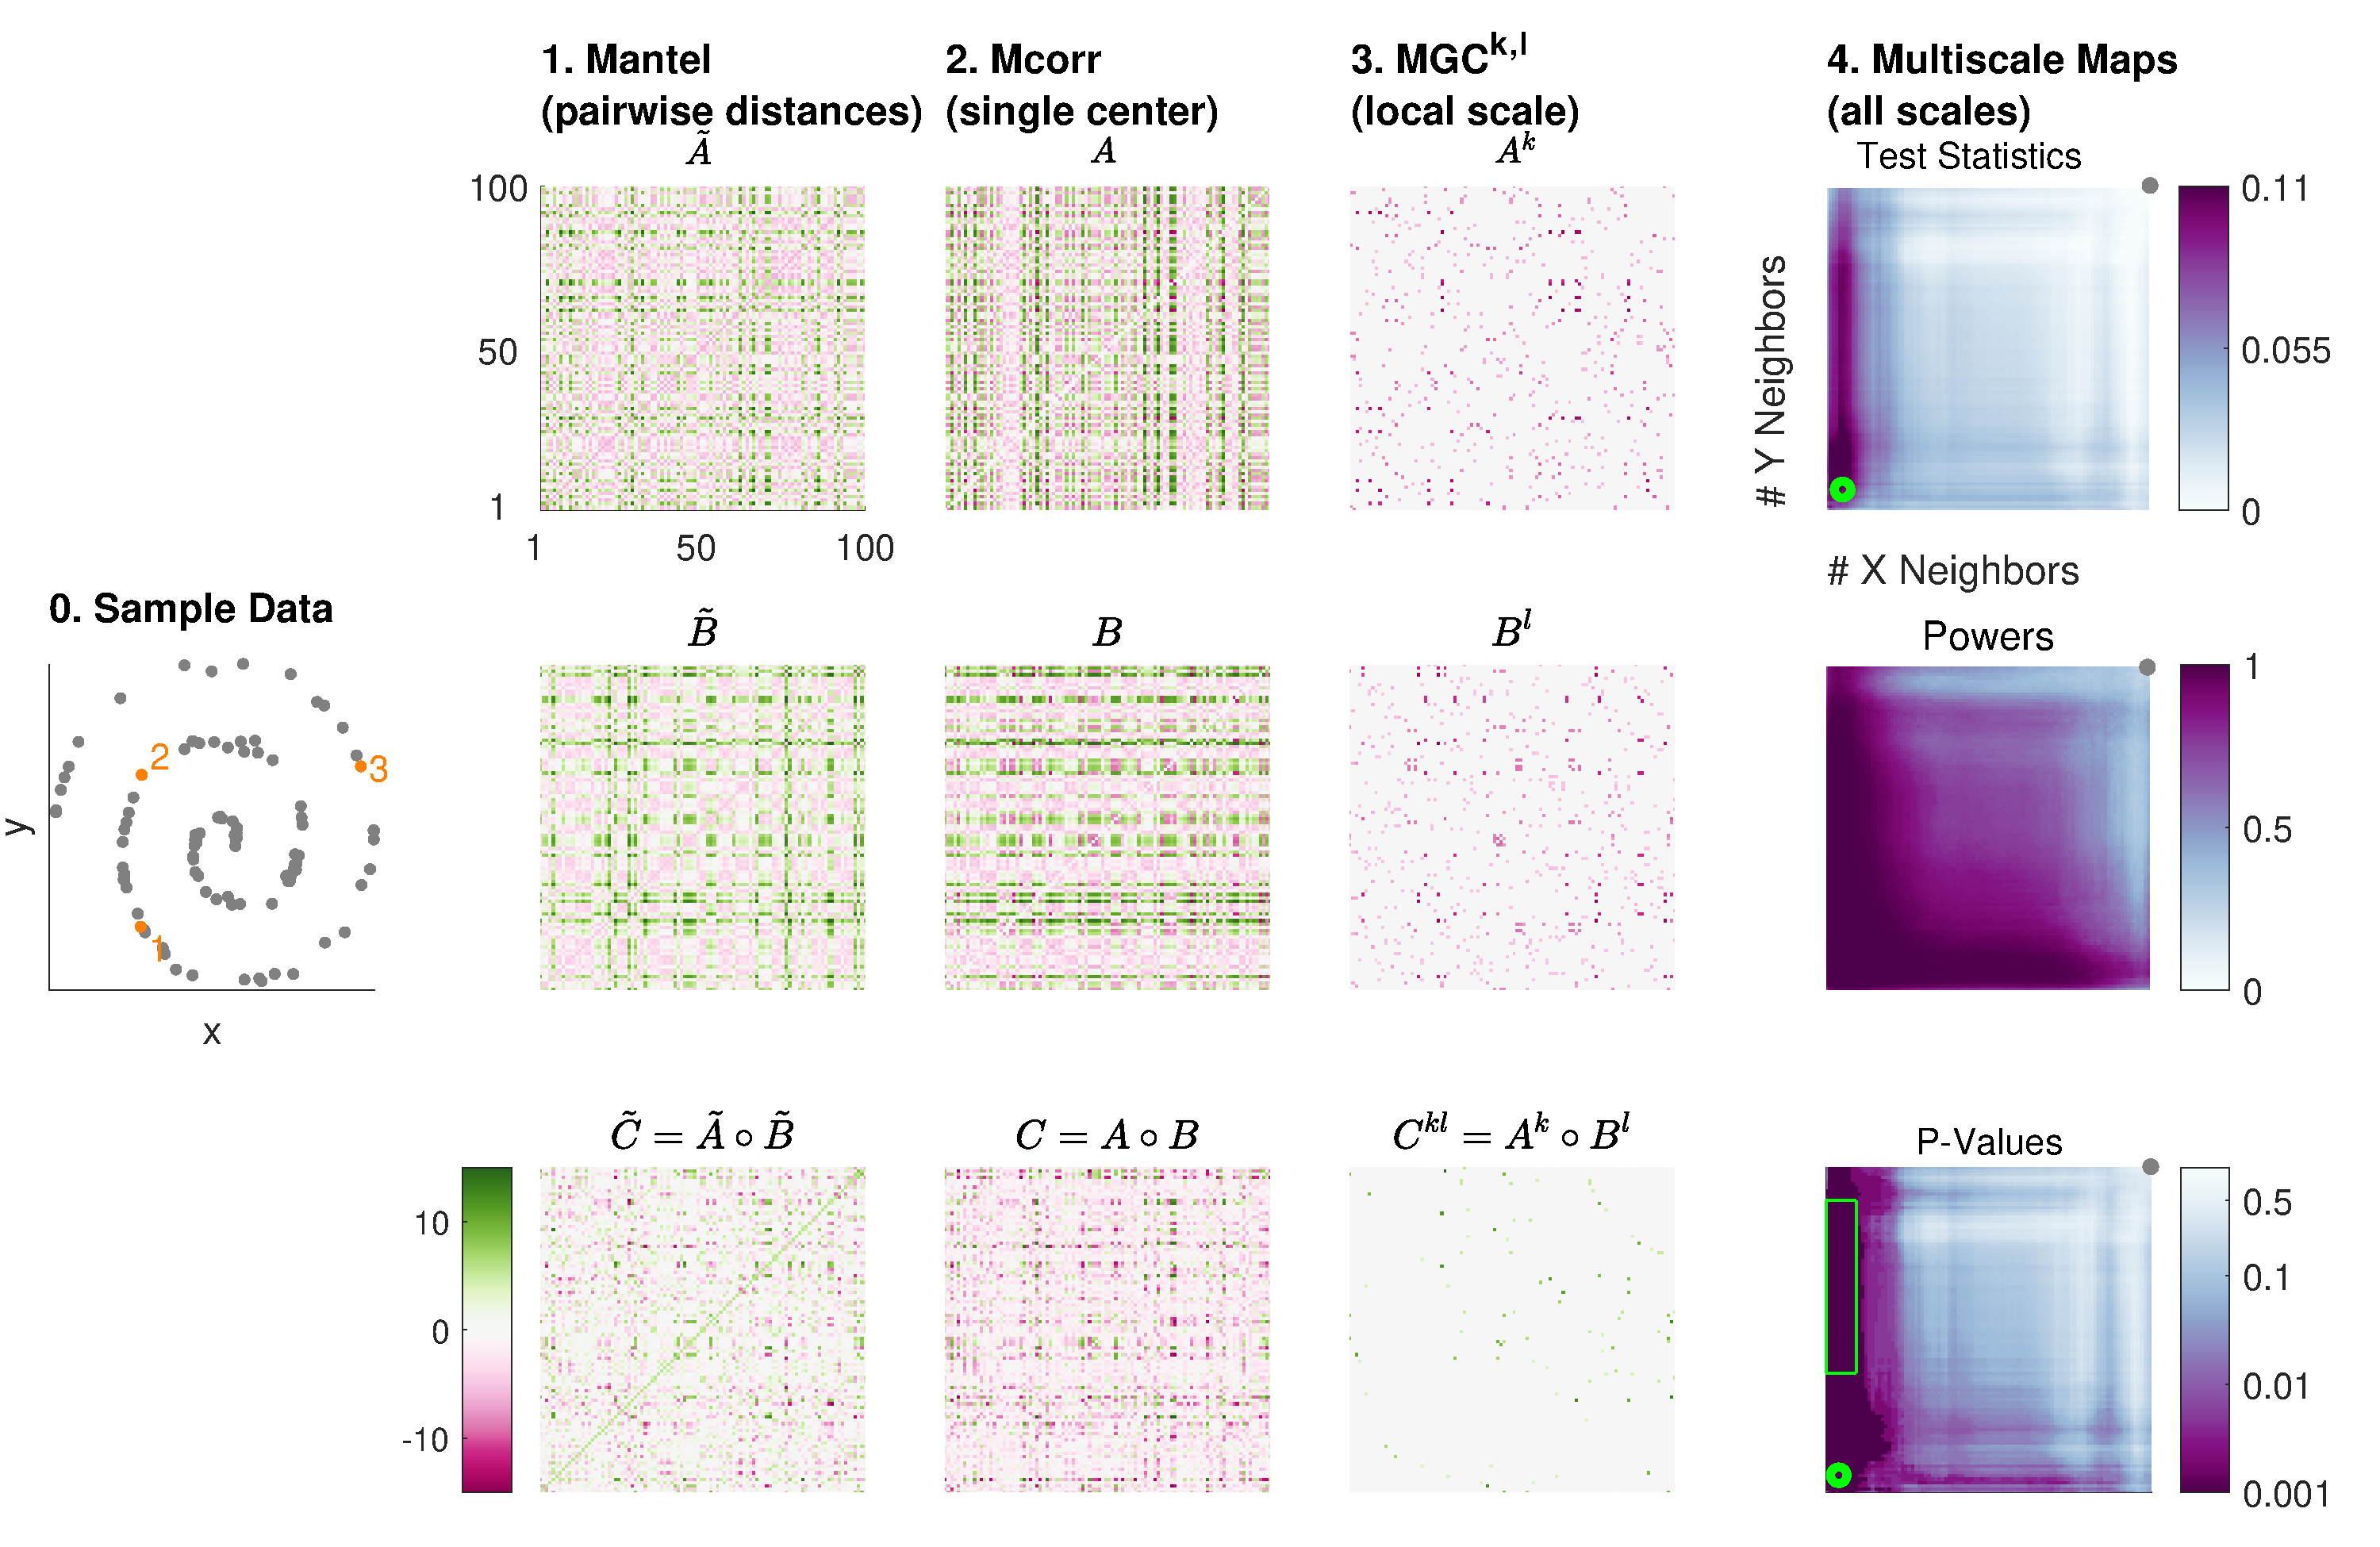
\includegraphics[width=1.0\textwidth,trim={0 0 2cm 0},clip]{Figures/FigA}
\setlength{\tabcolsep}{10pt} % Default value: 6pt
\begin{tabular}{r r r r}
\multicolumn{1}{l}{{\small \textbf{6. Table}}} & & & \\
$\delta_x$(1,2)   & \hspace{1.5em} \color{magenta}-1.75  & \hspace{3.5em} \color{magenta}-2.66  &  \hspace{3.0em} \color{magenta}-2.66  \\ 
 $\delta_y$(1,2) & \color{magenta}-2.00 & \color{magenta}-2.27 & \color{magenta}-2.27  \\ 
 $\delta_x \times \delta_y$ & \color{green}3.51 & \color{green}6.05 & \color{green}6.05  \\ 
 
\hline

 $\delta_x$(2,3) & \color{green}4.48 & \color{green}3.45 & 0.00  \\ 
 $\delta_y$(2,3) &  \color{magenta}-0.86 & \color{magenta}-0.26 & 0.00  \\ 
 $\delta_x \times \delta_y$ & \color{magenta}-3.87 & \color{magenta}-0.88 & 0.00  \\ 

\hline
 $\sum{\delta_x \times \delta_y}$ & \color{magenta}-147.18   & \color{green}7.06 & \color{green}159.72  \\ 
 test statistic &  \color{magenta}-0.02  & 0.00 & \color{green}0.24  \\  
\end{tabular}

\begin{tikzpicture}[remember picture,overlay]
\node[xshift=-5.2cm,yshift=-0.6cm] at (current page.east){%
    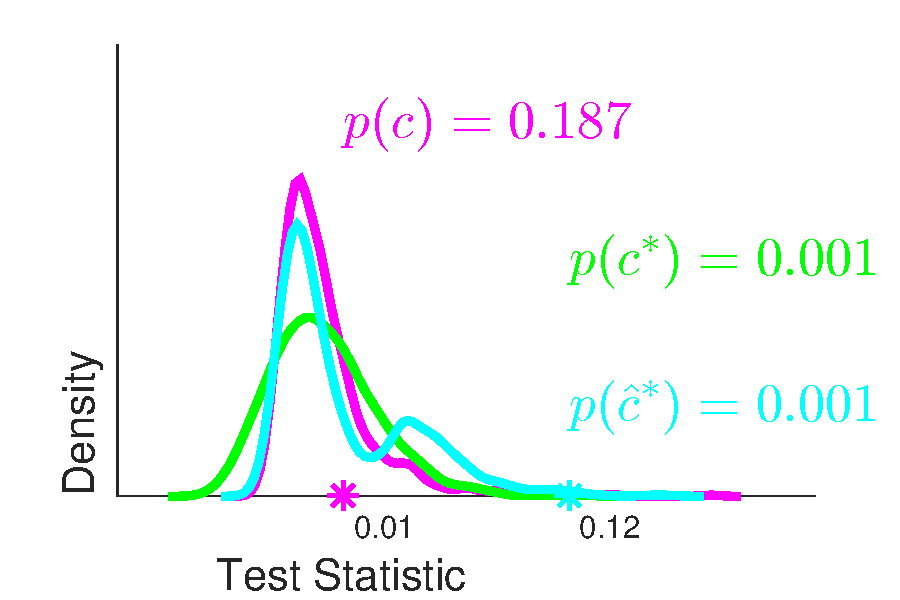
\includegraphics[width=0.35\textwidth,trim={1.5cm 0 1.8cm 0},clip]{Figures/FigB}};
  %\node[anchor=east,inner sep=0pt] at ($(current page.east)-(10cm,10cm)$) {
   %  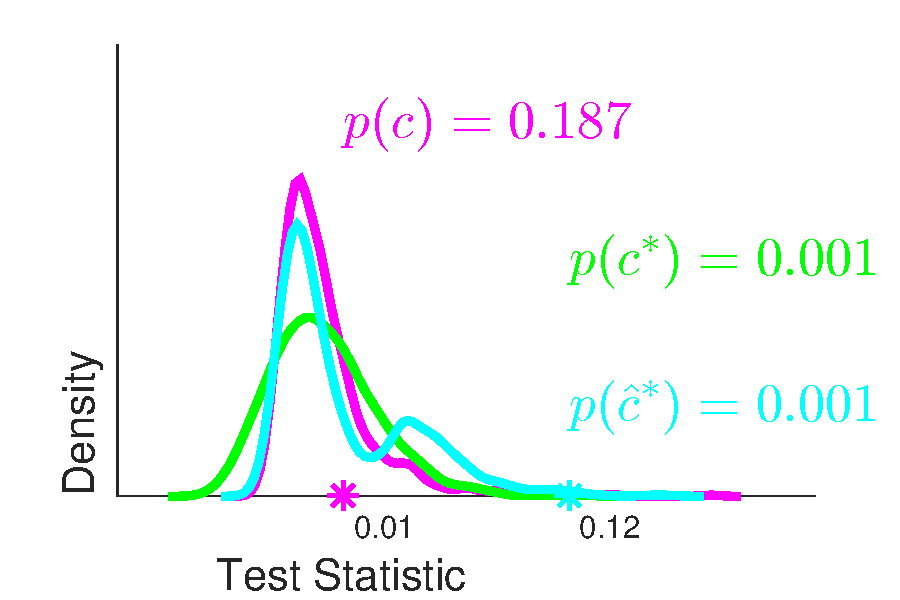
\includegraphics[width=0.3\textwidth]{Figures/FigB}
  %};
\end{tikzpicture}
\caption{
Schematic  and table demonstrating the ability of Multiscale Generalized Correlation (\Mgc) to detect dependence in nonlinear settings. 
\textbf{0.} 50 pairs of observations $(x_i,y_i)$ are nonlinearly (spirally) dependent on one another.
% 
\textbf{1.} Choose a metric on $x$ and another on $y$, and compute all pairwise distances (centered by the overall means) for $x$ and $y$ yielding interpoint comparison matrices
 $\tilde{A}$ (top) and $\tilde{B}$ (middle), 
and their element-wise products $\tilde{C}=\tilde{A} \circ \tilde{B}$ (bottom), whose normalized sum is the  \Mantel~statistic \cite{Mantel1967} (bottom row of table).
% 
\textbf{2.} Single centering --- subtract the row-sums from $\tilde{A}$ and column-sums from $\tilde{B}$ to eliminate bias due to individual samples --- yields $A=\{a_{ij}\}$ and $B=\{b_{ij}\}$; the normalized sum of their  element-wise product  $C$ is equivalent to the  \Mcorr~statistic \cite{SzekelyRizzo2013a}.
% 
\textbf{3.} Given a local scale, for example, $k=l=4$ here, yields $A^{k}$, $B^{l}$, and $C^{kl}$.  All these test statistics are normalized sums of the element-wise products. The fact that \Mgc~yields a $C^{kl}$ matrix that is all positive, whereas the others yield $C$ matrices with both positive and negative values, suggest that \Mgc~will correctly report a large test statistic here, resulting in a small p-value.
\textbf{4.} Compute the test statistics (top), power (middle), and p-value (bottom) for all local scales, resulting in multiscale maps that reveal the  scales of dependency. 
\textbf{5.} Report the corresponding observed test statistics and p-values, and discover the optimal scales (green rectangle in  p-value map) by Sample \Mgc.  
Whereas \Mcorr, the global test, has very low power (magenta dot in  p-value map) and therefore yields a small statistic and a non-significant p-value ($0.348$),  there are many local scales that achieve nearly perfect power, so both Oracle and Sample \Mgc~($\G^{*}$ and $\hat{\G}^{*}$) obtain large test statistics and highly significant p-values ($\approx 0.001$) and reveal the scales of dependency. 
\textbf{6.} Numerical demonstration of how \Mgc~is able to detect dependence even in highly nonlinear and low-sample size settings. The three colored points in the scatter plot indicate the three points considered in this table. 
The global methods fail to detect significant dependence since they consider all pairs, including the non-local ones, which \emph{negatively} impact the degree of dependence estimated.
\Mgc~only considers pairs that are jointly local (such as $(1,2)$), while discarding other pairs (such as $(2,3)$). 
}
\label{f:schematic}
\end{figure}

\begin{figure}[htbp]
% 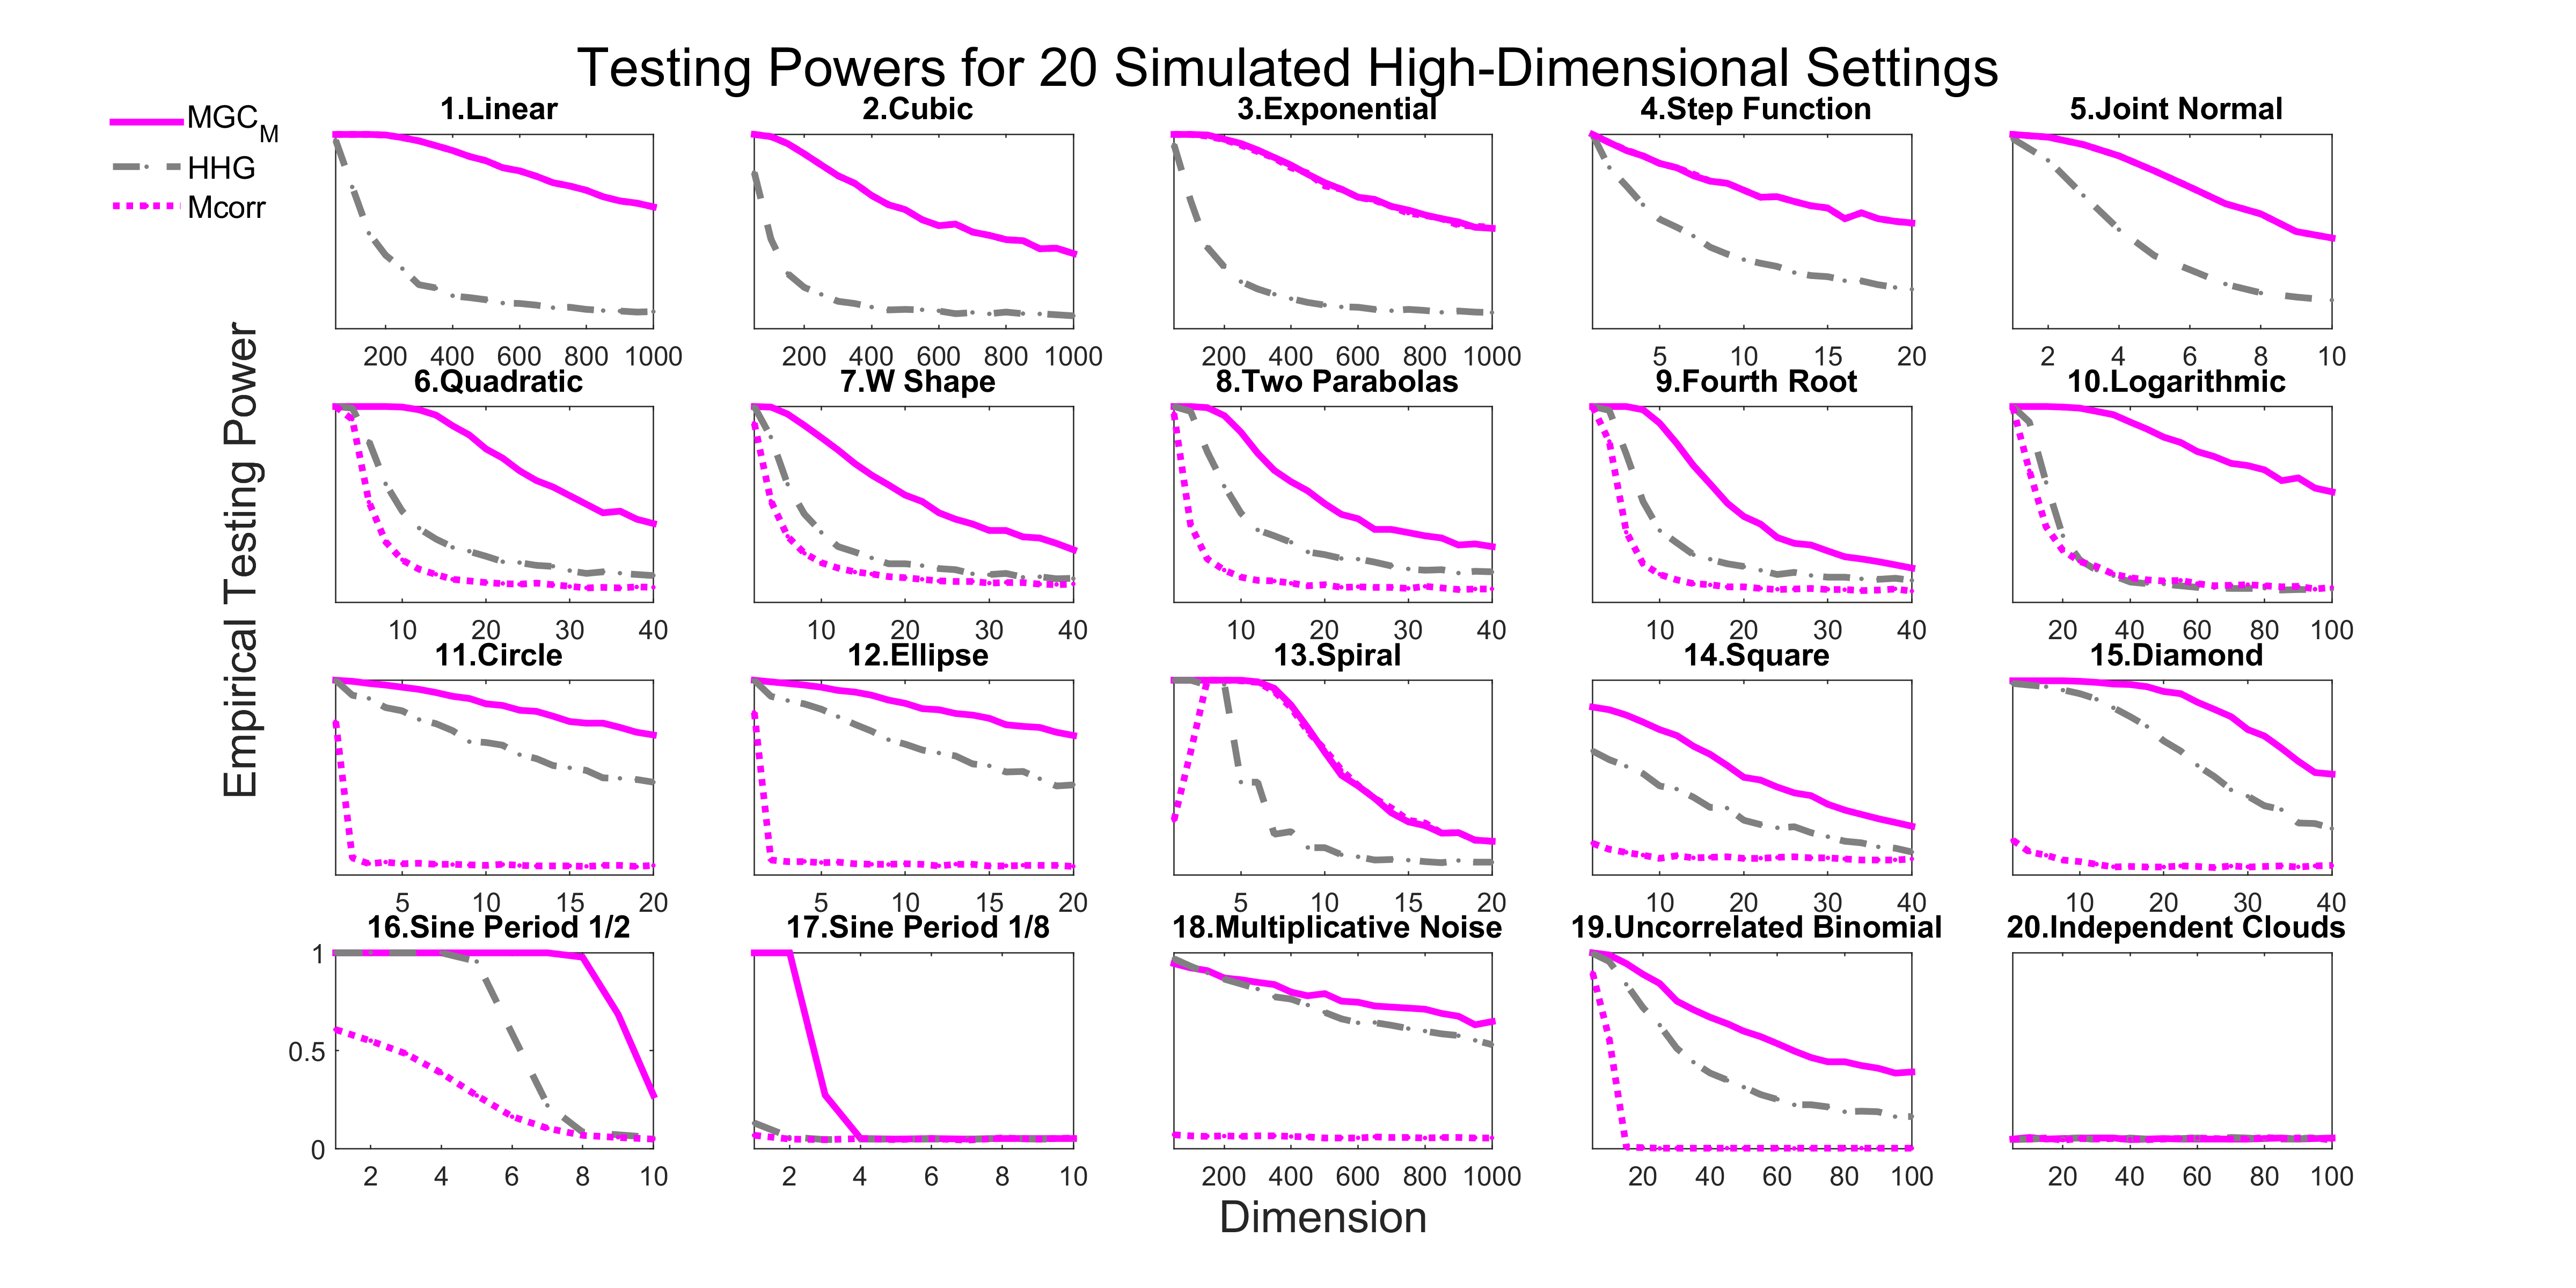
\includegraphics[width=1.0\textwidth,trim={0 0.5cm 4cm 0},clip]{Figures/FigHDPower}
\caption{Power of Oracle \Mgc, Sample \Mgc, \Mcorr, and \Hhg~for $20$ different dependence settings, estimated by Monte Carlo independence tests (see Algorithm \ref{alg:power} in Supplementary \ref{appen:algorithms} for details).  
Each panel shows the testing power at significance level $\alpha=0.05$
% \jv{should we include `# of' or just leave it off? technically, isn't everything "# of"?}
versus the dimensionality of $\mb{x}$'s, for $n=100$ samples (the dimensionality of $y$ increases for some settings, see Supplementary \ref{appen:function} for details). 
Excluding the independent  setting (\#20), for which all methods yield power $0.05$, as they should, \Mgc~empirically achieves similar or better power than both \Mcorr~\cite{SzekelyRizzo2013a}, its global counterpart, and \Hhg~\cite{HellerGorfine2013}, another state-of-the-art method, for almost all settings and all dimensions. 
}
\label{f:nD}
\end{figure}


\begin{figure}[htbp]
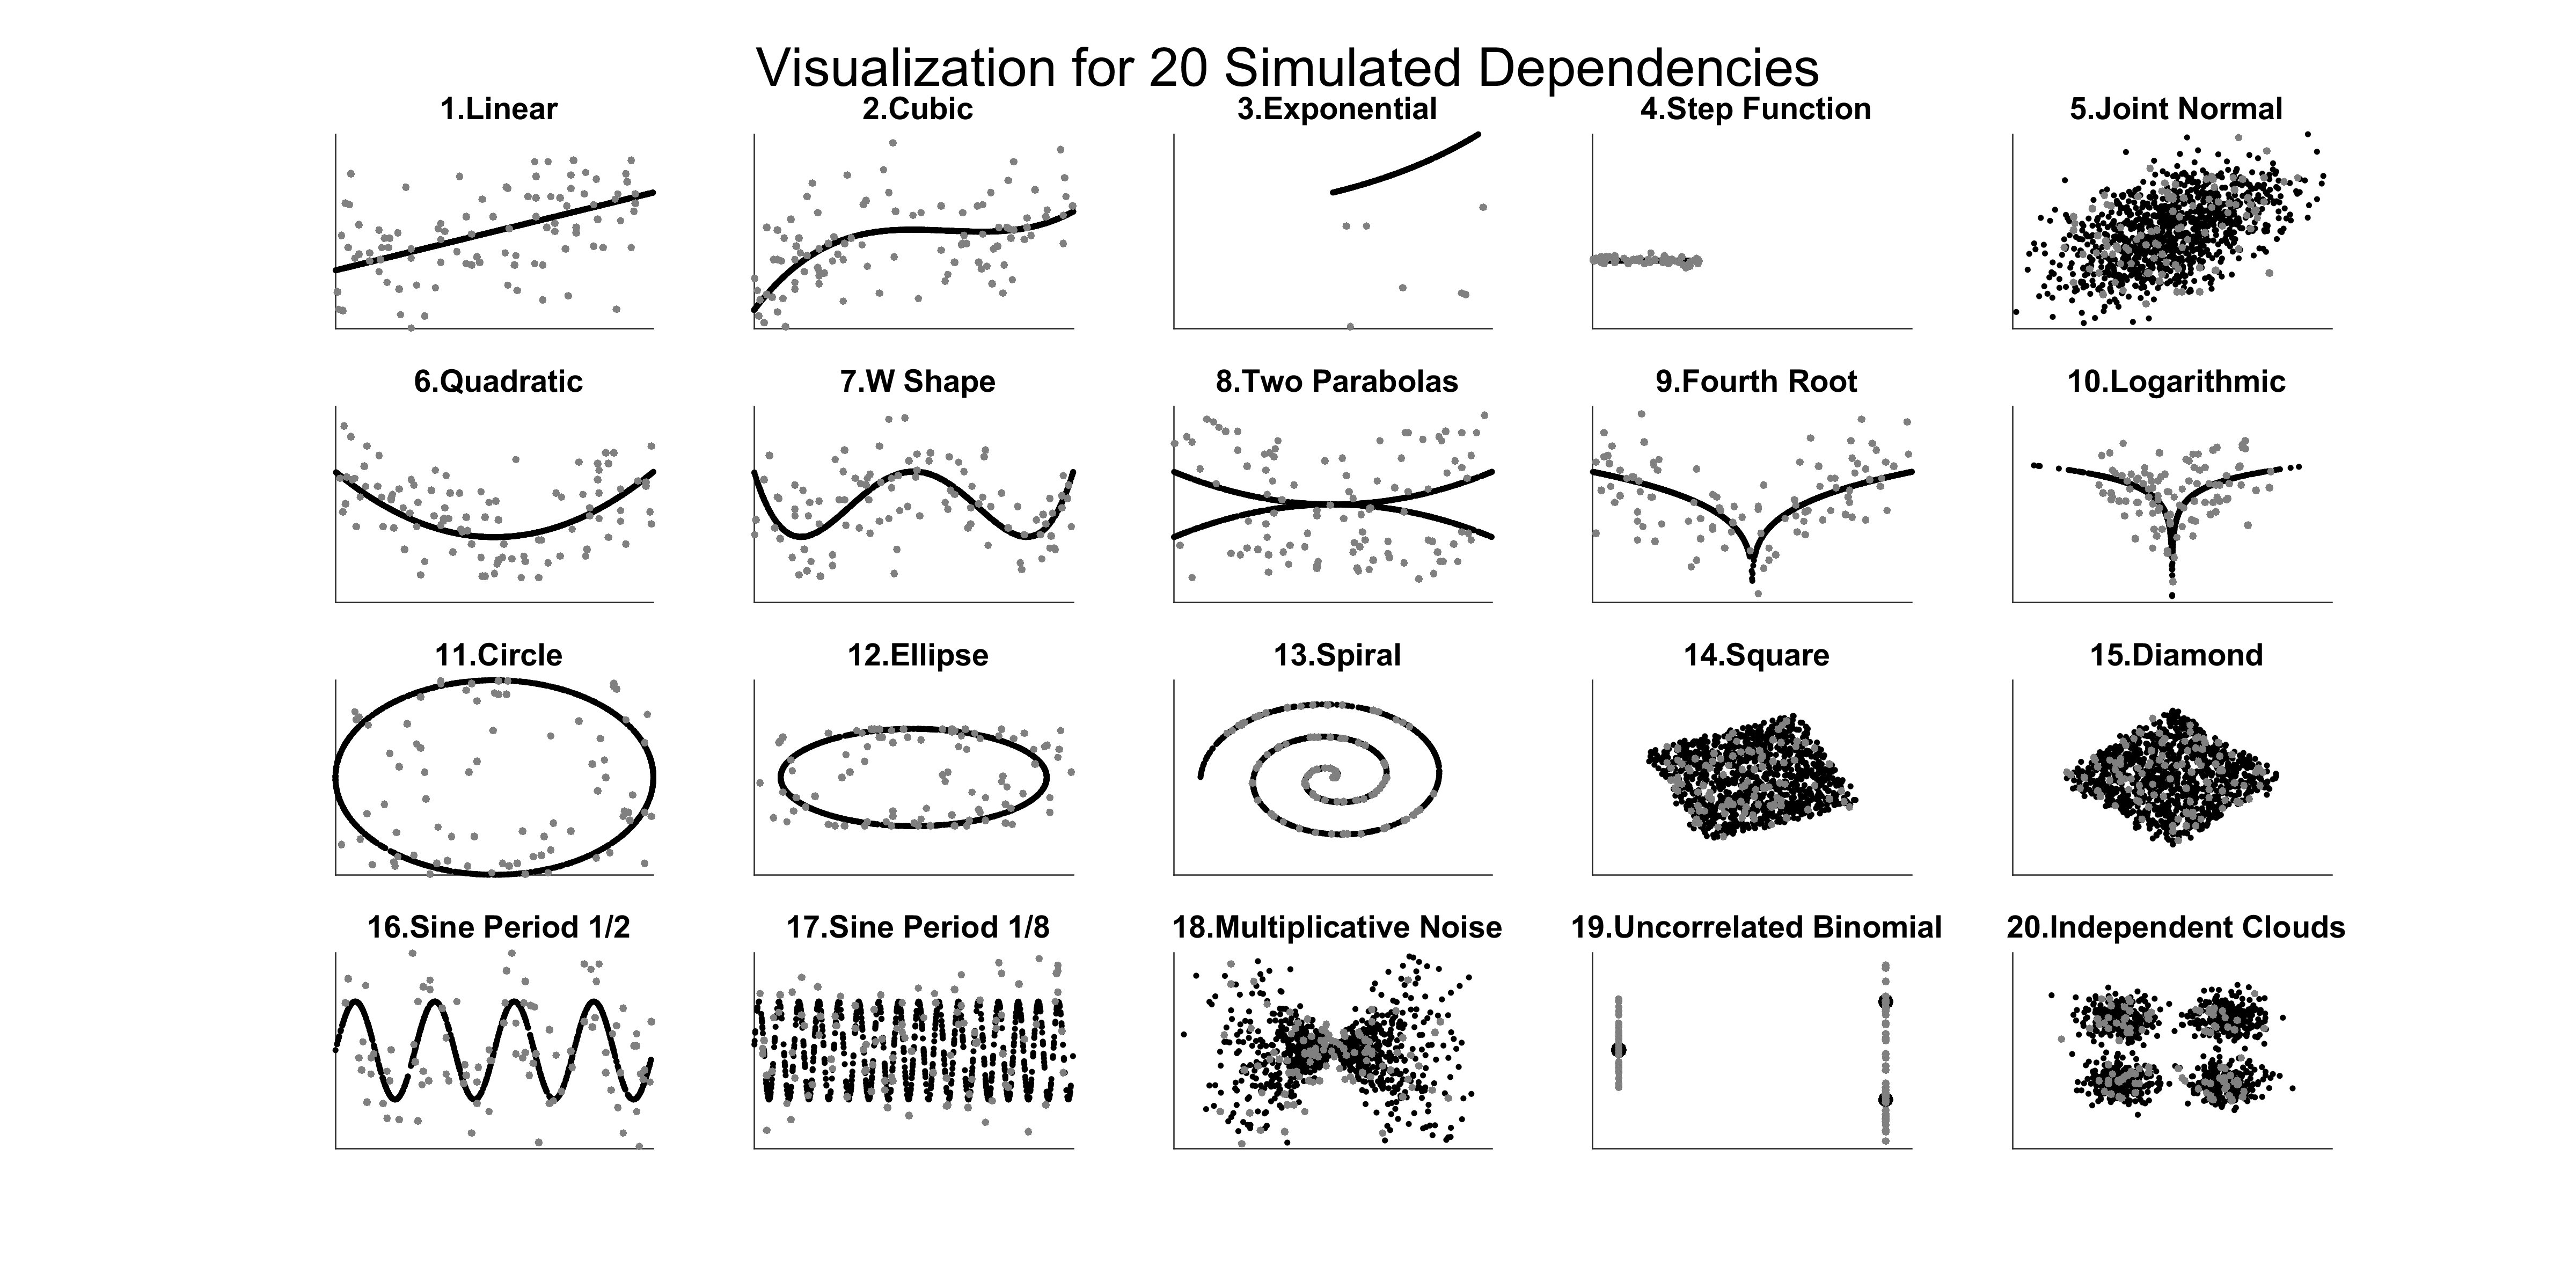
\includegraphics[trim={5cm 1.5cm 4cm 0.5cm},clip, width=1.0\textwidth]{Figures/FigSimVisual}
\caption{Visualization of the $20$ dependencies at $D=D_{y}=1$. For each, we sampled $n=100$ points with noise ($c=1$) to show the actual sample data used for 1-dimensional settings (gray dots). For comparison purposes, we also sampled $n=1000$ points without noise ($c=0$) to highlight each underlying dependency (black dots).
}
\label{f:dependencies}
\end{figure}

\begin{figure}[htbp]
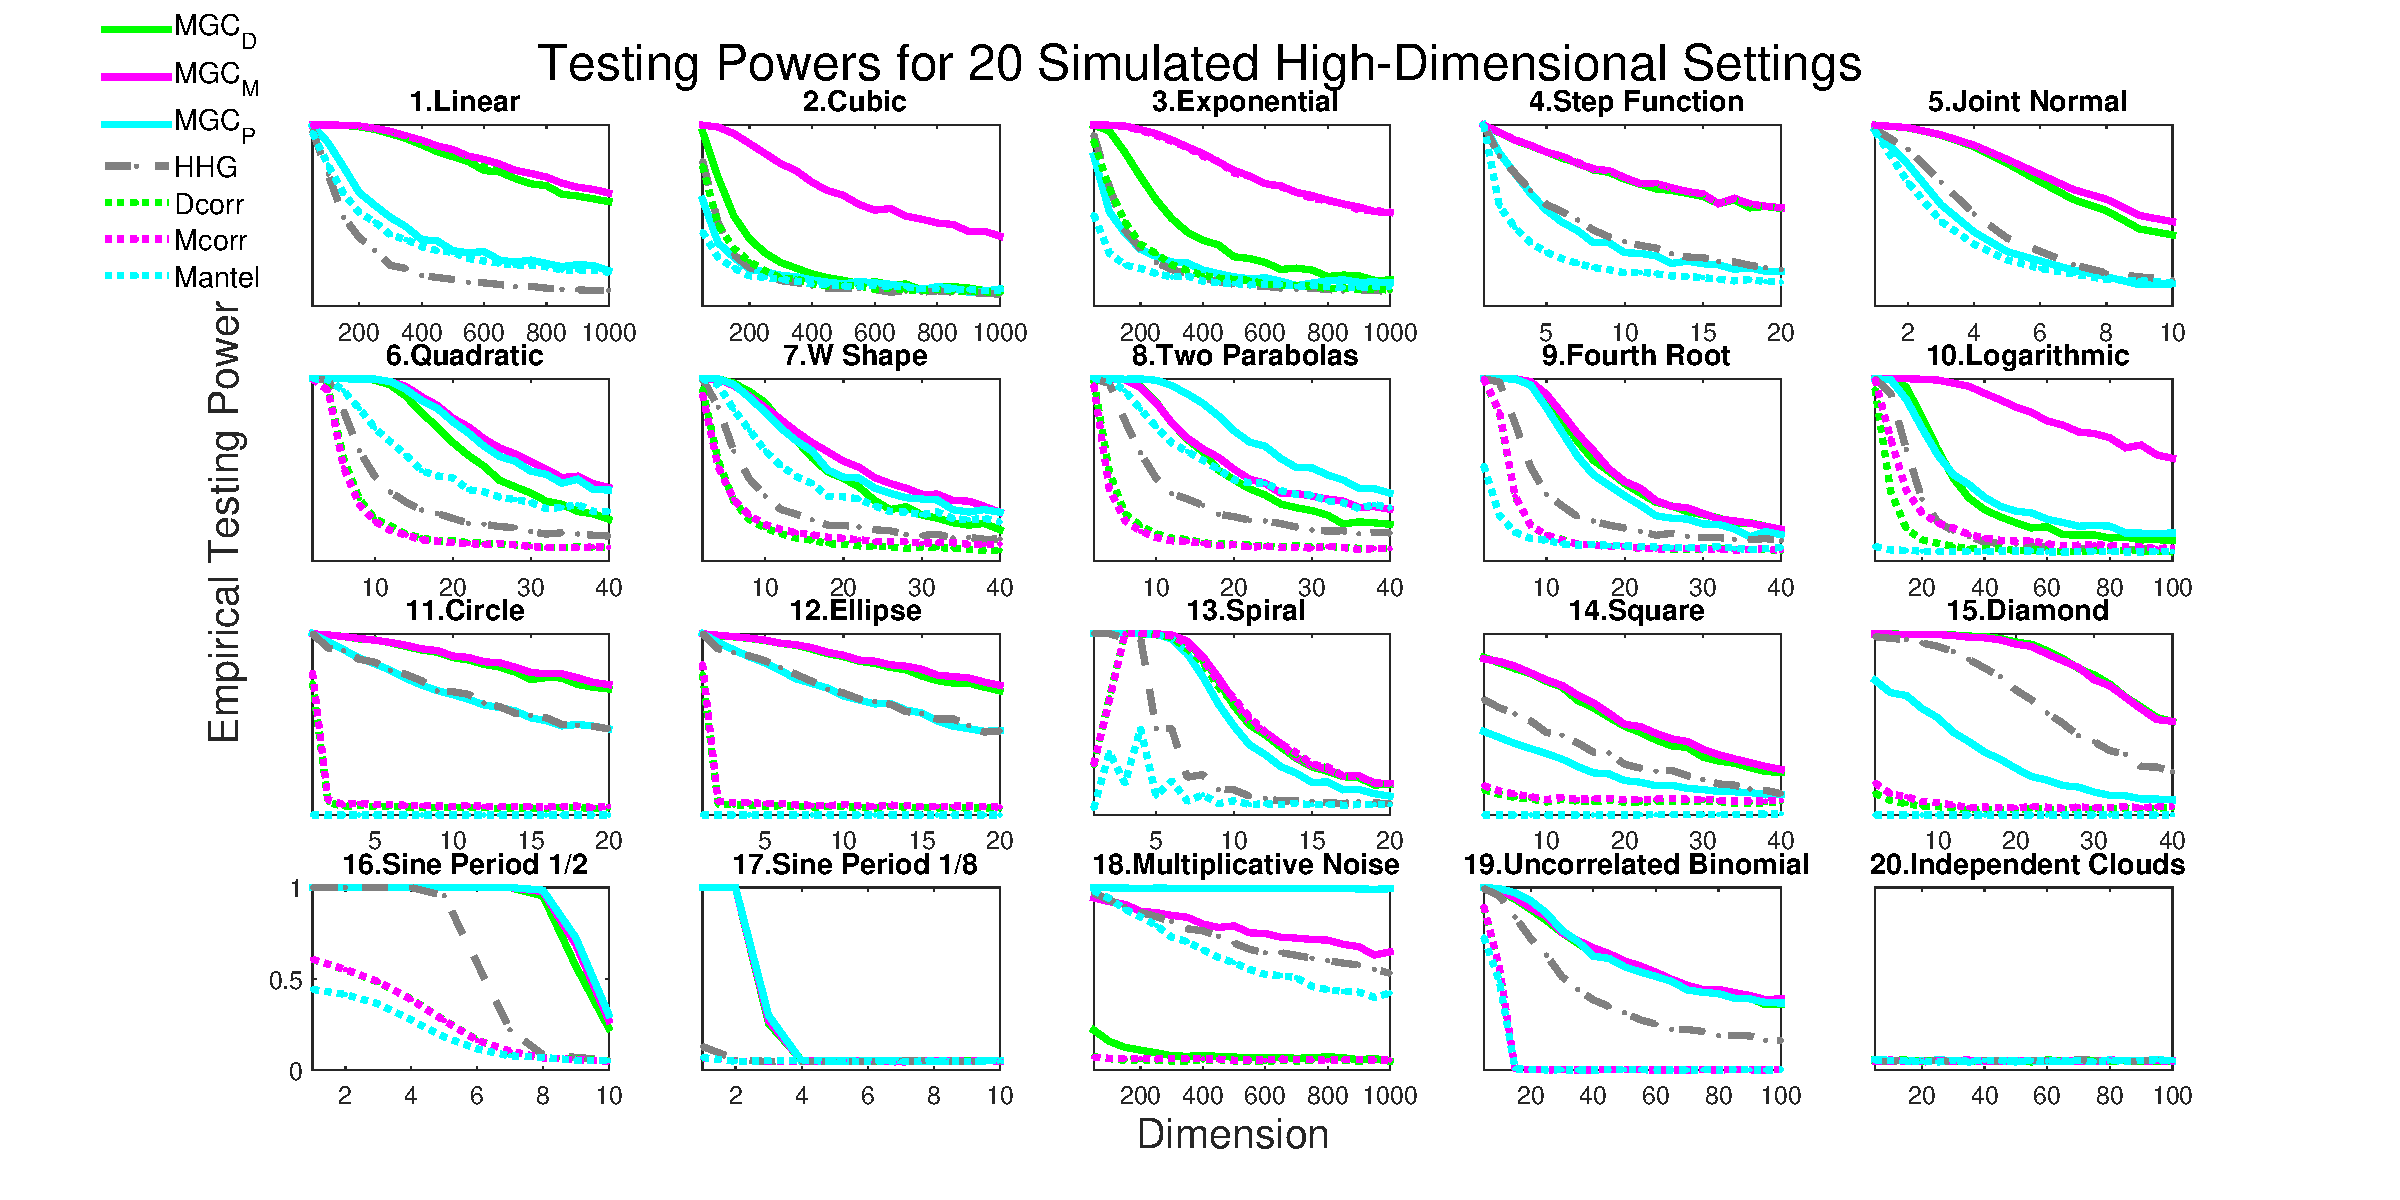
\includegraphics[width=1.0\textwidth,trim={0 0.5cm 4cm 0},clip]{Figures/FigHDPowerAll}
\caption{Power of different methods for $20$ different dependence settings, estimated by Monte Carlo independence tests (see Algorithm \ref{alg:power} for details). It includes eight different tests: \Mcorr, \Dcorr, and \Mantel~(gray solid, dashed, and dashdot lines, respectively), their corresponding Oracle \Mgc~counterparts, \Mgcm, \Mgcd, \Mgcp~(green with same line styles), Sample \Mgc~by \Mcorr~(cyan solid), and \Hhg~(gray dotted line). 
Each panel shows the testing power at significance level $\alpha=0.05$ versus the dimensionality of $\mb{x}$'s, for $n=100$ samples. 
Excluding the independent setting (\#20), for which all methods yield power $0.05$, as they should, Oracle \Mgc~empirically achieves similar or better power than the respective global counterpart. In particular, Sample \Mgc~is very close to Oracle \Mgcm, and overall dominates existing approaches for almost all settings and all dimensions, including \Hhg~\cite{HellerGorfine2013}, another state-of-the-art method. Note that \Mgc~is always plotted ``on top'' of the global variants if there is overlap, therefore, some of the global variants are not always visible from the display.}
\label{f:nDAll}
\end{figure}

\begin{figure}[htbp]
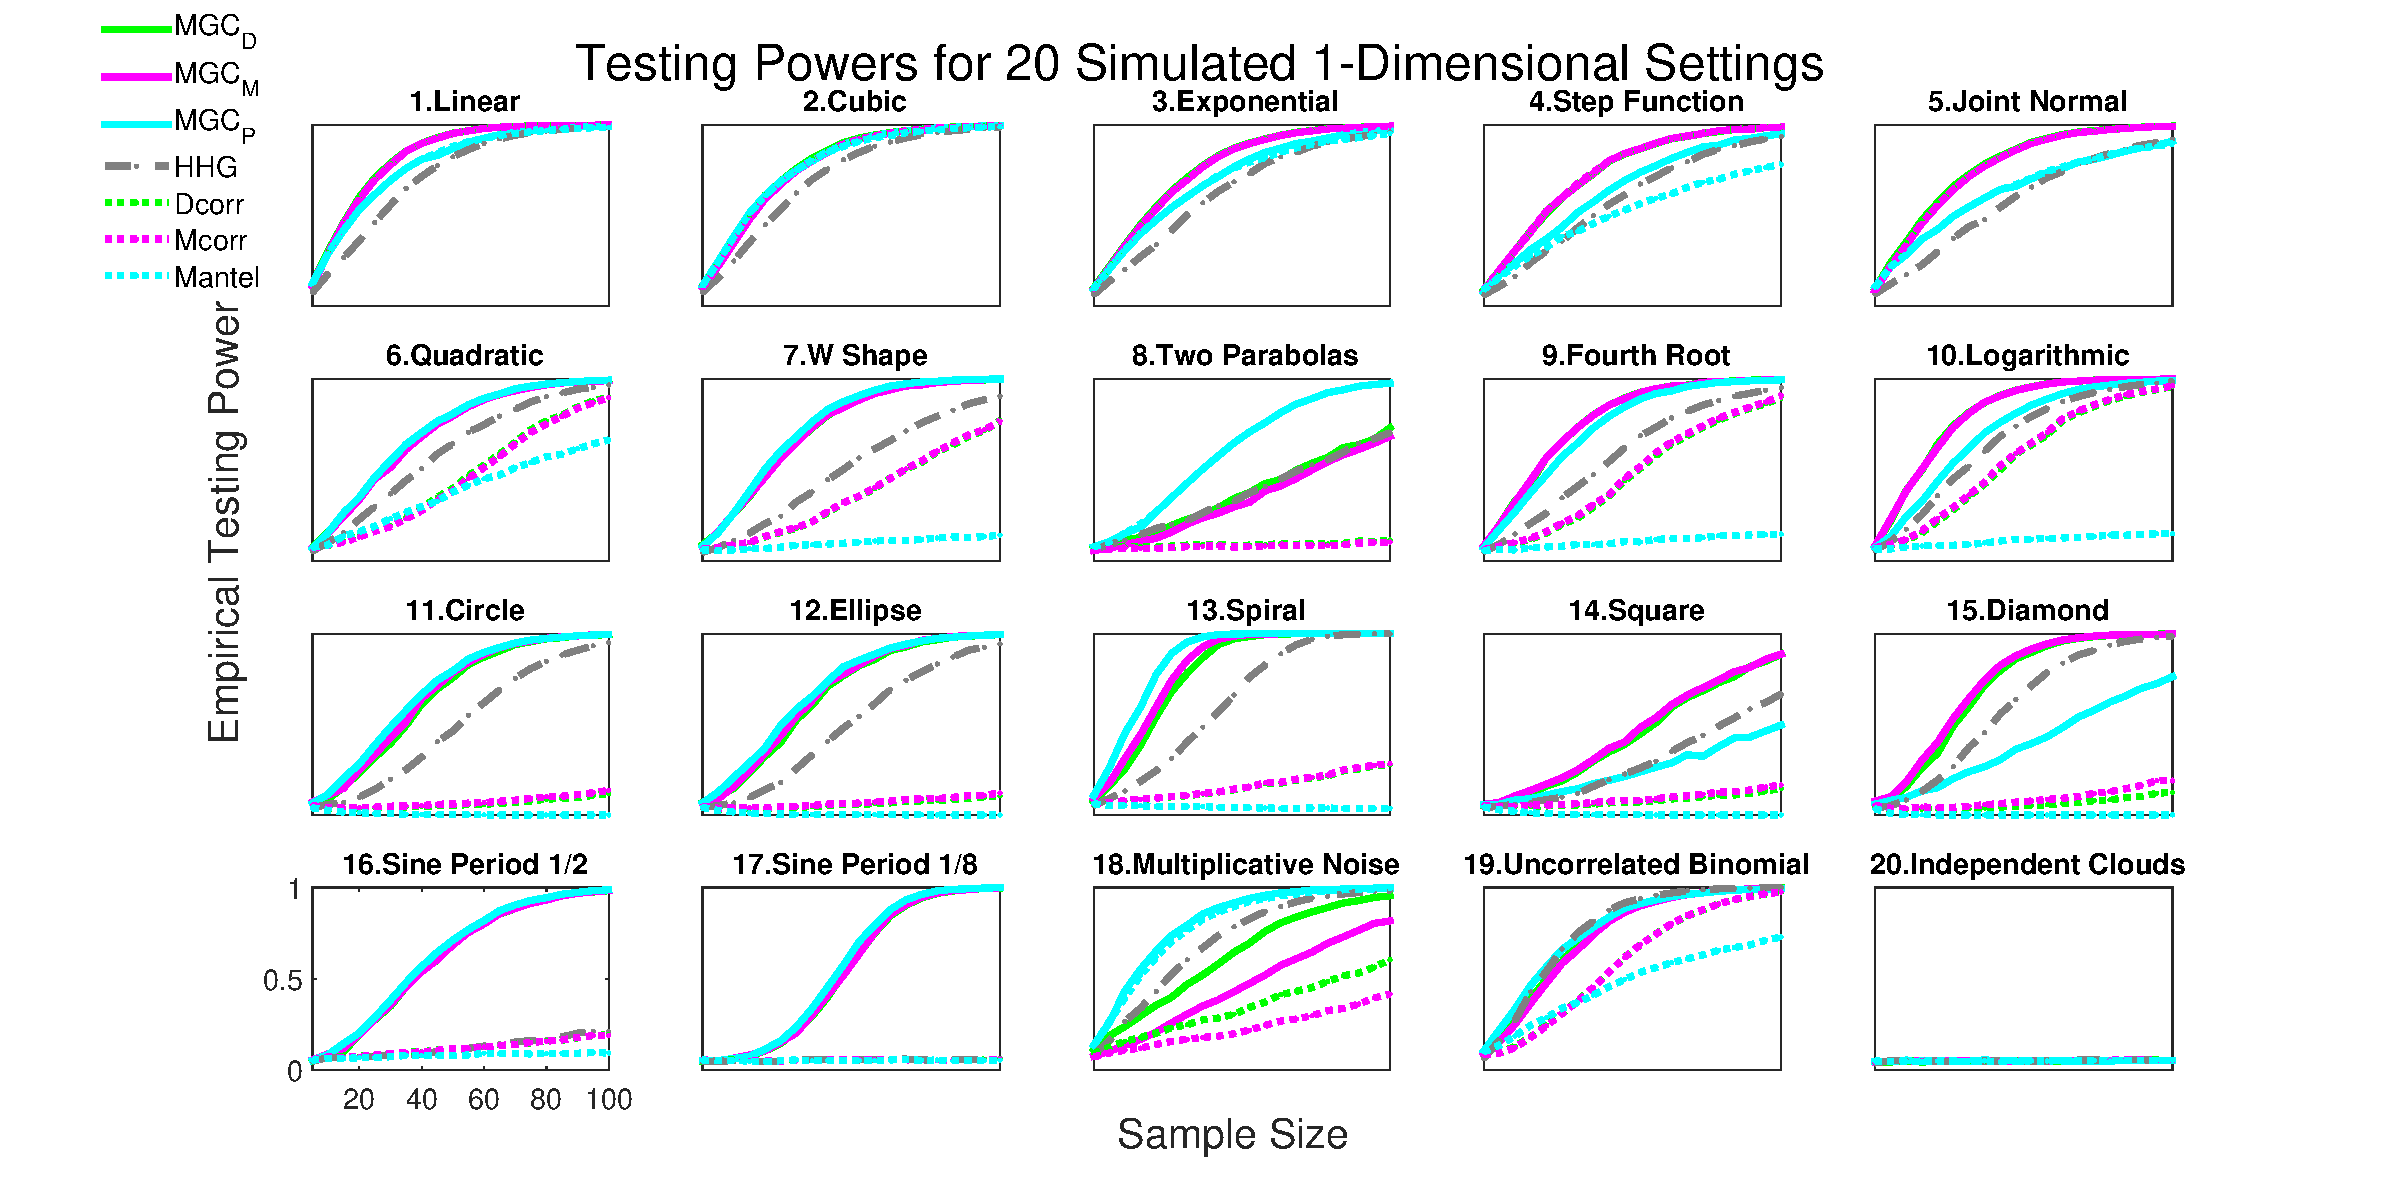
\includegraphics[width=1.0\textwidth,trim={0 0.5cm 4cm 0},clip]{Figures/Fig1DPowerAll}
\caption{
The same power plots as in Figure~\ref{f:nDAll}, except the $20$ dependence settings are one-dimensional with noise.
Each panel shows the testing power on the abscissa at a significance level $\alpha=0.05$, and sample size on the ordinate.
Again, Oracle \Mgc~empirically achieves similar or better power than the previous state of the art approaches for all sample sizes on almost all problems, with Sample \Mgc~being very close to Oracle \Mgc~and overall superior to other benchmarks.}
\label{f:1DAll}
\end{figure}

\begin{figure}
  \centering
  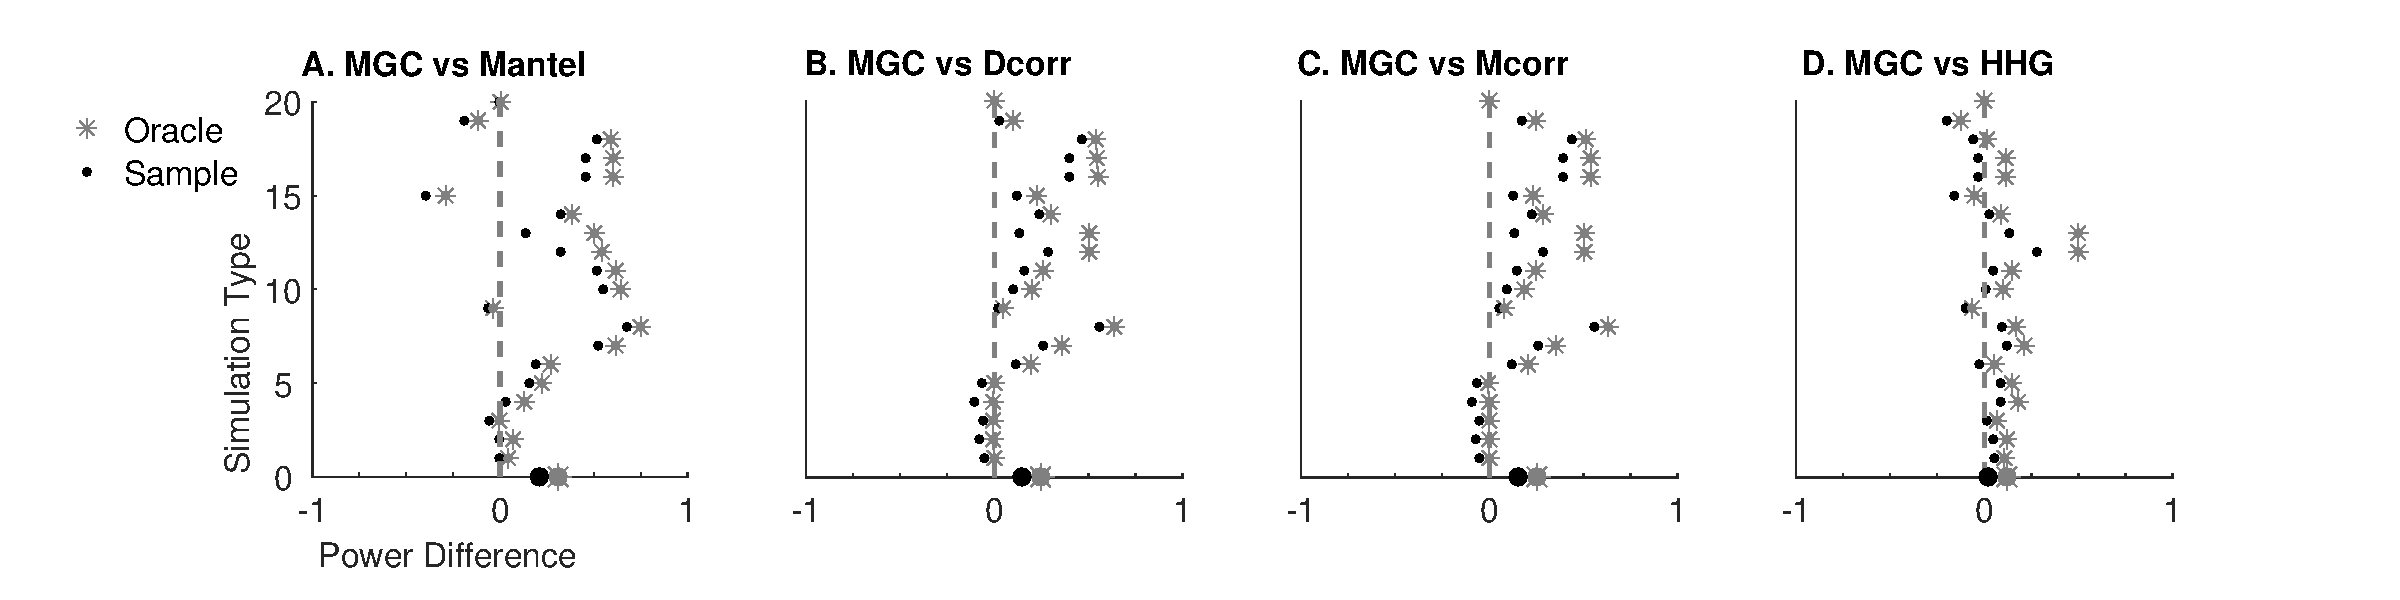
\includegraphics[width=1.0\textwidth,trim={1cm 0 3cm 0},clip]{Figures/Fig1DPowerMGCM}
  \caption{The same summary figure as Figure~\ref{f:nDSummary}, but based on the testing power of the $20$ $1$-dimensional simulation settings in Figure~\ref{f:1DAll}. 
  \Mgc~is again the most superior methods, exhibiting mean power slightly over \Hhg~for most settings, and very significant advantage over \Mantel, \Dcorr, \Mcorr~for most nonlinear dependencies.}
\label{f:1DSummary}
\end{figure}


\begin{figure}[htbp]
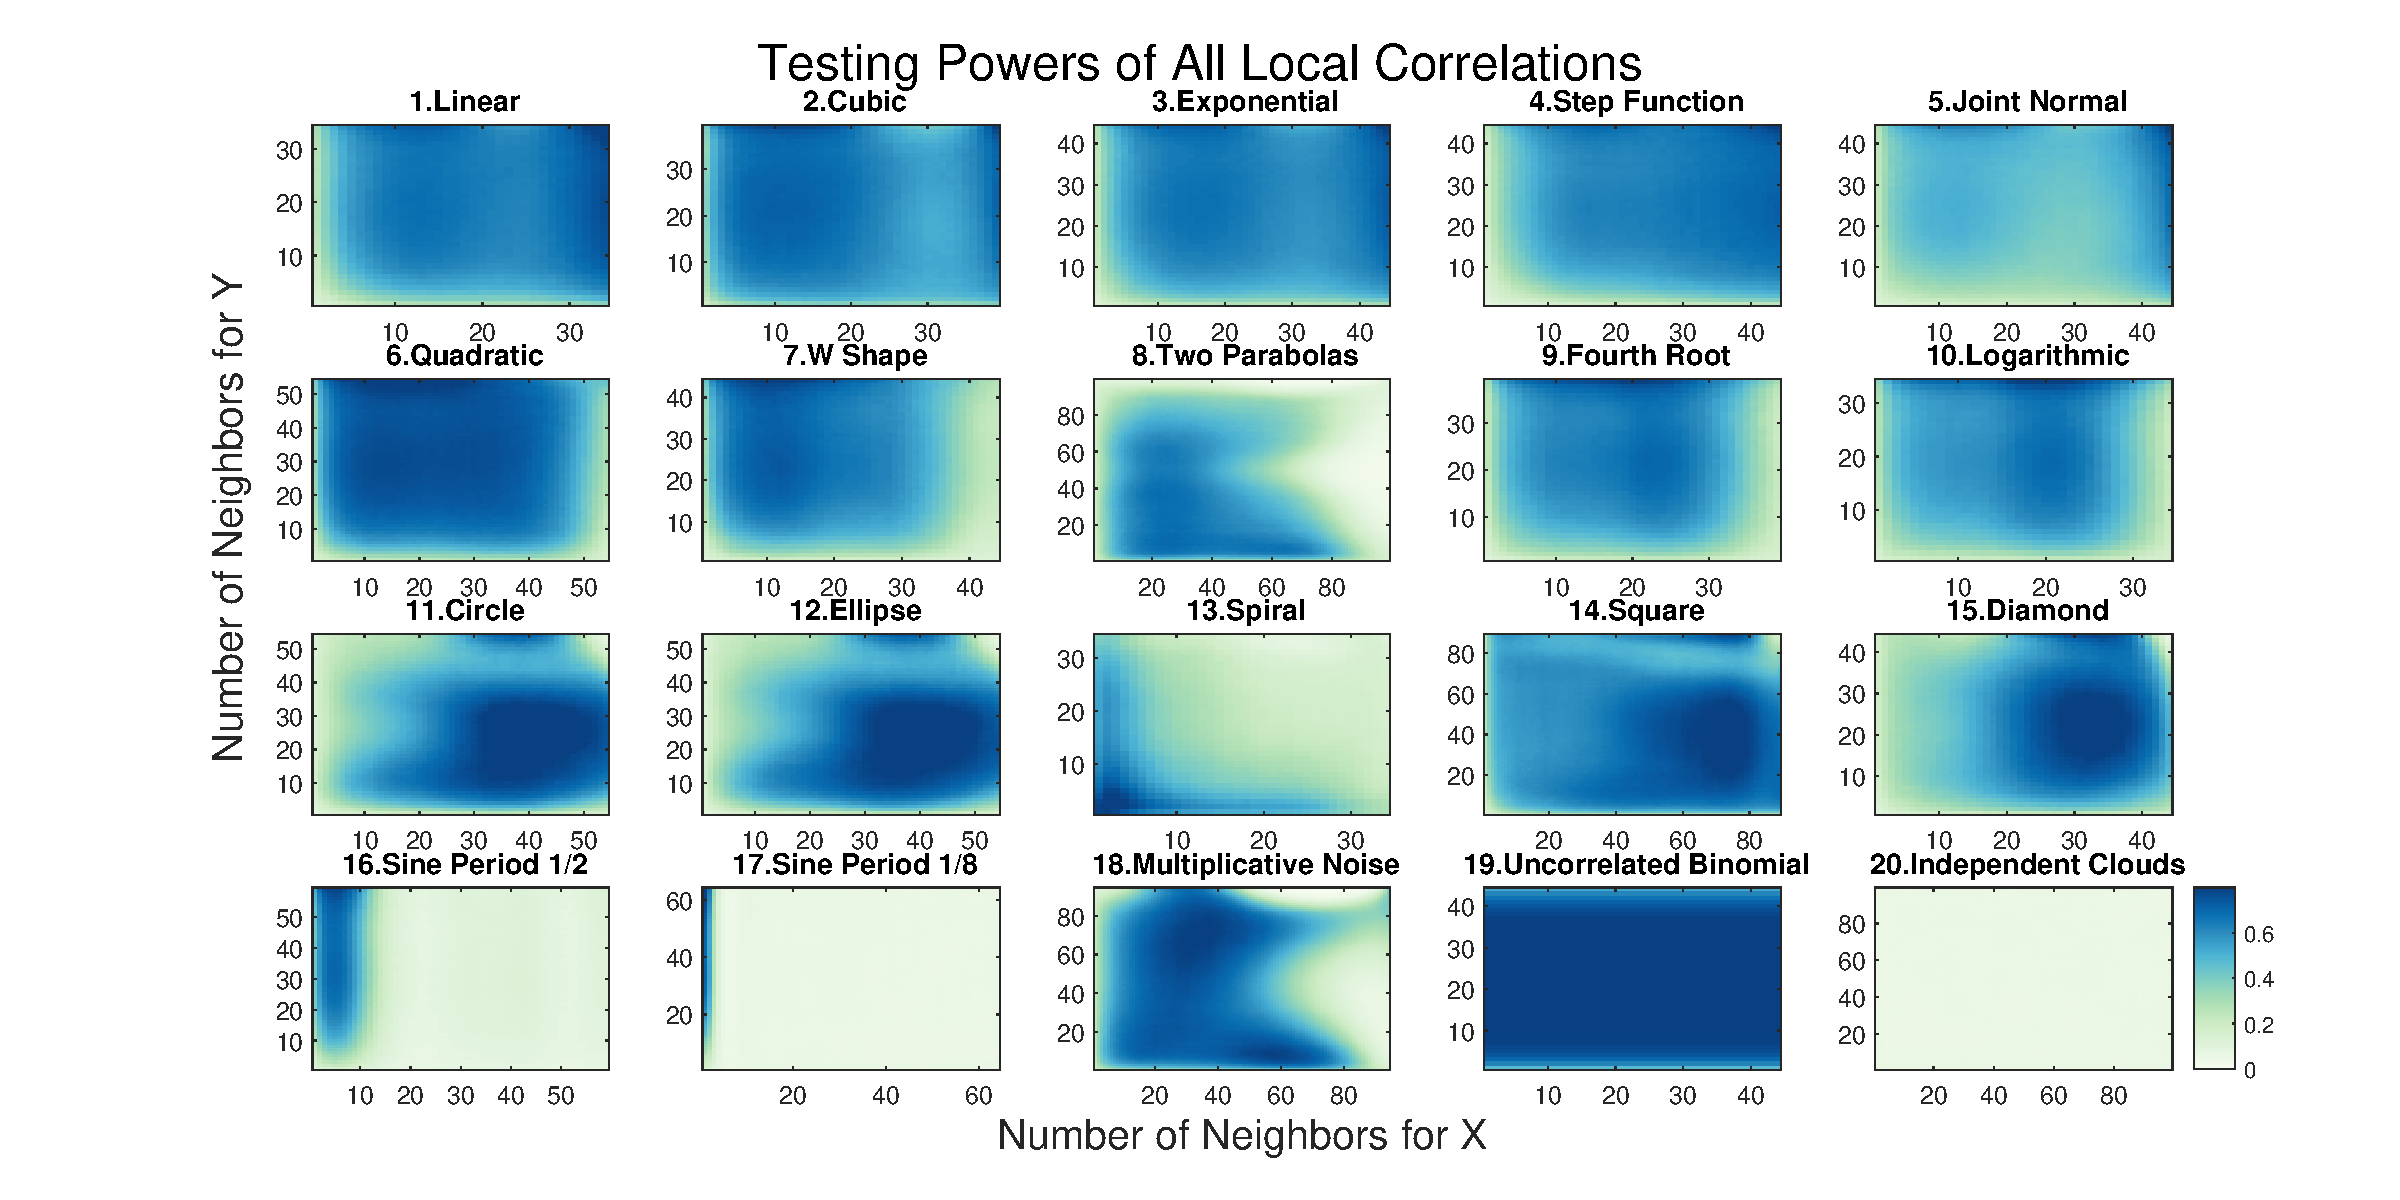
\includegraphics[width=1.0\textwidth,trim={3cm 0.5cm 2.5cm 0.5cm},clip]{Figures/Fig1DHeat}
\caption{Multiscale Power Maps indicating the influence of neighborhood size on \Mgc~testing power, for the one-dimensional simulations in Figure~\ref{f:1DAll}. For each simulation,  the sample size is $n=60$, and the significance level is $\alpha=0.05$. For the (nearly) linear settings, the global scales achieve optimal power.  However, for the other nonlinear dependence settings, local scales always outperform the global scale.}
\label{f:powermaps1}
\end{figure}

\clearpage

\section{\Mgc~Algorithms and Testing Procedures}
\label{appen:tests}
In this section, we elaborate on the algorithms for computing all local correlations, Oracle and Sample \Mgc, the optimal scale estimation, as well as the testing power and p-value computations.

Six algorithms are presented in Supplementary~\ref{appen:algorithms}: 
Algorithm~\ref{alg:mgc} shows how \Mgc~can be applied to any two pairs of sample observations, to yield the correlation measure, the permutation p-value, the multiscale maps, and the optimal scales.
Algorithm~\ref{alg:sample_mgc} is the actual Sample \Mgc~algorithm. It finds the optimal correlation by thresholding and smoothing on the multiscale correlation map, which is an estimation of the Oracle \Mgc~.
Algorithm~\ref{alg:power} computes the testing power of all local statistics when the underlying joint distribution is known, which yields the multiscale power map. Then the optimal scales of Oracle \Mgc~can be accurately calculated by maximizing the power map.
Algorithm~\ref{alg:pval} computes the p-values of all local correlation by the random permutation test, which yields the multiscale p-value map. The p-value and the optimal scale estimation of Sample \Mgc~follow in this algorithm as well. 
Algorithm~\ref{alg:1scale} computes the local correlation coefficient at a given scale $(k,l)$, for a given choice of the global correlation coefficient.
Algorithm~\ref{alg:all_scales} provides an efficient method to compute all local correlations simultaneously, in the same running time complexity as computing one local correlation. 

\subsection{Algorithms}
\label{appen:algorithms}

All algorithms are implemented in Matlab and R with the algorithm shown below. For ease of presentation, we assume there are no repeating observations of \mbx~or \mby, and assume \Mcorr~is the global correlation.


\begin{algorithm}
\caption{Multiscale Generalized Correlation (\Mgc)}
\label{alg:mgc}
\begin{algorithmic}%[1]
\Require $n$ samples of $(x_i,y_i)$.
\Ensure The estimated MGC statistic $\hat{\G}^*$, its' p-value $p(\hat{\G}^*)$, the p-value map for all local correlations, and the estimated optimal scales, $\mathcal{S}$.
\Function{MGC}{$(x_i,y_i)$, for $i \in [n]$}
\Statex{\textbf{(1)} Calculate all pairwise distances}
\For{$i,j:=1,\ldots,n$}
\State  $a_{ij} = \delta_x(x_i,x_j)$ 
\Comment{$\delta_x$ is the distance between pairs of $x$ samples}
\State  $b_{ij} = \delta_y(y_i,y_j)$
\Comment{$\delta_y$ is the distance between pairs of $y$ samples}
\EndFor
\State Let $A=\{ a_{ij}\}$ and $B=\{ b_{ij}\}$.
% 
\Statex{\textbf{(2)} Calculate Multiscale Correlation Map \& Test Statistic}
\For{$k,l:=1,\ldots,n$}
\State  $\G^{kl}=\textsc{LocalCorr}(A,B)$ 
% $ = \frac{1}{z_{kl}} \sum_{ij} a^k_{ij} b^l_{ij}$
\Comment{local correlation for all scales}
\EndFor
\State Let $C=\{ \G^{kl}\}$.
\State Find $\hat{\G}^*=\textsc{MGCTestStatistic}(C)$ 
\Comment{estimated optimal test statistic}
% 
\Statex{\textbf{(3)} Null Distribution \& P-Values}
\For{$j:=1,\ldots,r$}
\State Let $\pi=\textsc{RandPerm}(n)$. \Comment{generate a random permutation of size $n$}
\State Repeat \textbf{(2)} using $A$ and $B(\pi,\pi)$ to obtain the null distribution, $C_{0}[j]$ and ${\hat{\G}_{0}}^{*}[j]$.
\EndFor
\State $p(\hat{\G}^*)= \frac{1}{r}\sum_{j=1}^r \mb{I}(\hat{\G}^* < \hat{\G}^{*}_{0}[j])$.
\Comment{compute p-value of Sample MGC}
% 
\Statex{\textbf{(4)} Multiscale P-Value Map and Optimal Scales}
\For{$k,l := 1,\ldots, n$}
\State $p(\G^{kl}) = \frac{1}{r}\sum_{j=1}^r \mb{I}(\G^{kl} < \G^{kl}_{0}[j])$ 
\Comment{compute p-value for all scales}
\EndFor
\State Construct the binary map:    $\mathcal{E}^{kl} = 1 $ iff $  p(\G^{kl}) < p(\hat{\G}^*)$. \Comment{find estimated optimal scales}
\State $\mathcal{S}=$ the set of elements in the largest axis aligned rectangle in $\mathcal{E}$ containing only $1$'s.
\EndFunction
\end{algorithmic}
\end{algorithm}


\begin{algorithm}
\caption{Compute the Sample \Mgc~test statistic. It finds the largest connected region in the correlation map, such that each correlation is significant, i.e., larger than a certain threshold. To avoid correlation inflation by sample noise, it then computes Sample MGC as follows: for the largest correlation in the region, calculate the two minimal correlations along adjacent row scales and adjacent column scales, then take the larger one as the Sample MGC. If the region area is too small, or the estimated Sample MGC is no larger than the global, use the global correlation instead. The running time is $O(n^2)$.}
\label{alg:sample_mgc}
\begin{algorithmic}[1]
\Require All local statistics $\{\G^{kl}\} \in \Real^{n \times n}$.
\Ensure The Sample \Mgc~statistic $\hat{\G}^{*} \in \Real$.
\Function{MGCTestStatistic}{$\{\G^{kl}\}$}
\State $\tau_{1} \rto \sum_{\G^{kl}<0} (\G^{kl})^2 / \sum_{\G^{kl}<0} 1$ \Comment{variance of all negative local correlations away from $0$}
\State $\tau_{1} \rto \max\{0.01,\sqrt{\epsilon}\} \times 3.5$ \Comment{threshold based on negative correlations}
\State $\tau_{2} \rto \min\{2/n,0.05\}$ \Comment{threshold based on sample size}
\State $R_{kl} \rto \mb{I}(\G^{kl}>\max\{\tau_{1},\tau_{2}\})$ \Comment{find all correlations that are larger than the thresholds}
\State $R = \textsc{Connected}(R)$ \Comment{largest connected component of all significant correlations}
\State $\hat{\G}^{*} \rto \G^{nn}$ \Comment{use the global correlation by default}
\If{$\sum_{k,l} R_{kl} \geq \tau_{2} n$} \Comment{proceed when the significant region is sufficiently large}
\State $\Omega \rto \arg_{k,l}\{(\G^{kl}\geq \max_{R_{kl}=1} \G^{kl}) \cap (R_{kl}=1)\}$ \Comment{scales with largest correlation in $R$}
\State $\gamma=\textsc{Ceiling}(0.1n)$
\For{$(k',l') \in \Omega$}
\State $\eta_{1} \rto \min_{k \in [k'-\gamma,k'+\gamma]}\{\G^{kl'}\}$ \Comment{minimal correlation at given column along nearby rows}
\State $\eta_{2} \rto \min_{l \in [l'-\gamma,l'+\gamma]}\{\G^{k'l}\}$ \Comment{minimal correlation at given row along nearby columns}
\State $\eta \rto \max\{\eta_{1},\eta_{2}\}$
\Lineif{$\eta > \hat{\G}^{*}$}{ $\hat{\G}^{*} \rto \eta$}
\EndFor
\EndIf
\EndFunction
\end{algorithmic}
\end{algorithm}


\begin{algorithm}
\caption{For known distribution, compute the multiscale power map, and the test statistic and optimal scales for Oracle \Mgc. By repeatedly simulating samples by the joint distribution $f_{xy}$, sample data of size $n$ under the null and the alternative are generated for $r$ Monte-Carlo replicates. Then all local correlations under the null and the alternative hypotheses are computed by Algorithm~\ref{alg:all_scales}, followed by estimating the testing power at each local correlation. The optimal scales of Oracle \Mgc~can be found by the scales that maximizes the power map. The running time is $O(rn^2 \log n)$. In the simulations we use $r=2$,$000$ MC replicates to estimate the optimal scale, and another $r=10$,$000$ MC replicates to estimate the power. This algorithm can be similarly adapted to training data, for which the alternative statistic can be computed from the training data while the null statistic can be computed by permutation. Note that power computation for Sample \Mgc~or other benchmarks follows from the same algorithm, by plugging in the respective test statistic in the first loop without the optimal scale computation. }
\label{alg:power}
\begin{algorithmic}[1]
\Require A joint distribution $f_{xy}$, the sample size $n$, the number of MC replicates $r$, and the type $1$ error level $\alpha$.
\Ensure The power matrix $\beta \in [0,1]^{n \times n}$ for all local correlations, and the \Mgc~optimal scale $(k^{*},l^{*}) \in \mathbb{N} \times \mathbb{N}$.
\Function{TestingPower}{$f_{xy}$,$n$, $r$,$\alpha$}
\For{$j:=1,\ldots,r$}
\Linefor{$i:=[n]$}{$(X^{1}_{i},Y^{1}_{i}) \stackrel{iid}{\sim} f_{xy}$, $X^{0}_{i} \stackrel{iid}{\sim} f_{x}$, $Y^{0}_{i} \stackrel{iid}{\sim} f_{y}$} 
\Linefor{$Z:=A,B$}{$\tilde{Z}_{1}=\textsc{Dist}(Z_{1})$, $\tilde{Z}_{0}=\textsc{Dist}(Z_{0})$} 
\State $\{\G^{kl}_{1}\}[j]=\textsc{LocalCorr}(\tilde{A}_{1},\tilde{B}_{1})$ \Comment{calculate all local correlations under the alternative}
\State $\{\G^{kl}_{0}\}[j]=\textsc{LocalCorr}(\tilde{A}_{0},\tilde{B}_{0})$ \Comment{calculate all local correlations under the null}
\EndFor

\For{$k,l:=1,\ldots,n$}
\State $\omega_{\alpha} \rto \textsc{Cdf}_{1-\alpha}(\G^{0}_{kl}[j],j \in [r])$ \Comment{get the critical value by the empirical distributions}
\State $\beta_{kl} \rto \sum_{j=1}^{r}(\G^{1}_{kl}[j]>\omega_{\alpha}) / r$ \Comment{compute the power map}
\EndFor
\State $(k^{*},l^{*}) \rto \arg_{k,l}\max(\{\beta_{kl}\})$ \Comment{compute the optimal local scales}
\EndFunction
\end{algorithmic}
\end{algorithm}


\begin{algorithm}
\caption{Compute the multiscale p-value map, the p-value of Sample \Mgc, and the optimal scales. This algorithm uses a permutation test with $r$ random permutations, requiring $O(rn^2 \log n)$. Specifically, it computes the multiscale correlation maps and then the sample \Mgc~value for the given data and $r$ permuted resamples, then the p-value for each local correlation and sample \Mgc~follows by the permutation test.  Then, the optimal scales are estimated by taking the largest rectangle with local p-values no larger than the p-value of Sample \Mgc.  In the real data experiment we always set $r=10$,$000$. Note that the p-value computation for any other global generalized correlation coefficient follows from the same algorithm by replacing Sample \Mgc~with the respective test statistic.
}
\label{alg:pval}
\begin{algorithmic}[1]
\Require A pair of distance matrices $(\tilde{A},\tilde{B}) \in \Real^{n \times n} \times \Real^{n \times n}$, the number of permutations $r$.
\Ensure The p-value matrix $P \in [0,1]^{n \times n}$ for all local correlations, the p-value $p \in [0,1]$ for Sample \Mgc, and estimated \Mgc~optimal scale $(\hat{k}^{*},\hat{l}^{*}) \in \mathbb{N} \times \mathbb{N}$.
\Function{PermutationTest}{$\tilde{A}$,$\tilde{B}$,$r$}
\State $\{\G^{kl}\}=\textsc{LocalCorr}(\tilde{A},\tilde{B})$ \Comment{calculate the observed local correlations}
\State $\hat{\G}^{*}=\textsc{SampleMGC}(\{\G^{kl}\})$ \Comment{Sample \Mgc~statistic}
\For{$j:=1,\ldots,r$}
\State $\pi=\textsc{RandPerm}(n)$ \Comment{generate a random permutation of size $n$} 
\State $\{\G^{kl}_{0}\}[j]=\textsc{LocalCorr}(\tilde{A},\tilde{B}(\pi,\pi))$ \Comment{calculate the permuted test statistics}
\State $\hat{\G}^{*}_{0}[j]=\textsc{SampleMGC}(\{\G^{kl}_{0}\}[j])$ \Comment{calculate the permuted Sample \Mgc}
\EndFor

\Linefor{$k,l:=1,\ldots,n$}{$P_{kl} \rto \sum_{j=1}^{r}(\G^{kl} \leq \G^{kl}_{0}[j])/r$} \Comment{the p-value map}
\State $p \rto \sum_{j=1}^{r}\mb{I}(\hat{\G}^{*} \leq \hat{\G}^{*}_{0}[j])/r$  \Comment{the p-value map for Sample \Mgc}
\State $(\hat{k}^{*},\hat{l}^{*}) = \textsc{LargestRectangle}(P\leq p)$ \Comment{estimate the optimal scales}
\EndFunction
\end{algorithmic}
\end{algorithm}





\begin{algorithm}
\caption{Compute local test statistic for a given scale. This algorithm runs in $O(n^2)$ once the rank information is provided, which is suitable for \Mgc~computation if an optimal scale is already estimated. But it would take $O(n^4)$ if used to compute all local correlations. Note that for the default \Mgc~implementation by single centering, the centering function centers $\tilde{A}$ by column and $\tilde{B}$ by row, and the sorting function sorts $\tilde{A}$ within column and $\tilde{B}$ within row.}
\label{alg:1scale}
\begin{algorithmic}[1]
\Require A pair of distance matrices $(\tilde{A},\tilde{B}) \in \Real^{n \times n} \times \Real^{n \times n}$, and the given local scale $(k,l) \in \mathbb{N} \times \mathbb{N}$.
\Ensure The local correlation coefficient $\G^{kl} \in [-1,1]$ at the given $(k,l)$.
\Function{LocalCorr}{$\tilde{A}$,$\tilde{B}$,$k$,$l$}
\State Initialize $\G^{kl}$, $V^{A}_{k}$, $V^{B}_{l}$, $E^{A}_{k}$, $E^{B}_{l}$ at $0$.
\Linefor{$Z:=A,B$}{$R^{Z}=\textsc{Sort}(\tilde{Z})$} \Comment{sort distances}
\Linefor{$Z:=A,B$}{$Z=\textsc{Center}(\tilde{Z})$}  \Comment{center distance matrices}

\For{$i,j:=1,\ldots,n$}
\State $\G^{kl} \rto \G^{kl}+A_{ij}B_{ij}\mb{I}(R^{A}_{ij} \leq k)\mb{I}(R^{B}_{ij} \leq l)$ \Comment{update un-centered local distance covariance}
\Linefor{$Z:=A,B$}{$V^{Z}_{k} \rto V^{Z}_{k}+Z_{ij}^2\mb{I}(R^{Z}_{ij} \leq k)$} \Comment{update local distance variances}
\Linefor{$Z:=A,B$}{$E^{Z}_{k} \rto E^{Z}_{k}+Z_{ij}\mb{I}(R^{Z}_{ij} \leq k)$} \Comment{update sample means}
\EndFor

\State $\G^{kl} \rto \left(\G^{kl}-E^{A}_{k}E^{B}_{l}/n^2\right)/\sqrt{\left(V^{A}_{k}-{E^{A}_{k}}^2/n^2\right) \left(V^{B}_{l}-{E^{B}_{l}}^2/n^2\right)}$ \Comment{center and normalize} 

\EndFunction
\end{algorithmic}
\end{algorithm} 

\begin{algorithm}
\caption{Compute the multiscale correlation map in $O(n^2 \log n)$. Once the distances are sorted, this algorithm computes all local correlations in $O(n^2)$. An important observation is that each product $a_{ij}b_{ij}$ is included in $\G^{kl}$ if and only if $(k,l)$ satisfies $k\leq R(a_{ij})$ and $l\leq R(b_{ij})$, so it suffices to iterate through $a_{ij}b_{ij}$ for $i,j=1,\ldots,n$, and add the product simultaneously to all $\G^{kl}$ whose scales are no more than $(R(a_{ij}),R(b_{ij}))$. To achieve the above, we iterate through each product, add it to $\G^{kl}$ at $(k,l)=(R(a_{ij}),R(b_{ij}))$ only (so only one local scale is accessed for each operation); then add up adjacent $\G^{kl}$ for $k,l=1,\ldots,n$. The same applies to all local covariances, variances, and expectations.} 
\label{alg:all_scales}
\begin{algorithmic}[1]
\Require A pair of distance matrices $(\tilde{A},\tilde{B}) \in \Real^{n \times n} \times \Real^{n \times n}$.
\Ensure All local correlation coefficients $\{\G^{kl}\} \in [-1,1]^{n \times n}$ for $k,l=1,\ldots,n$.
\Function{LocalCorr}{$\tilde{A}$,$\tilde{B}$}
\State Initialize $C$ as a zero matrix of size $n \times n$; $V^{A}$, $V^{B}$, $E^{A}$, $E^{B}$ as zero vectors of size $n$.
\Linefor{$Z:=A,B$}{$R^{Z}=\textsc{Sort}(\tilde{Z})$}
\Linefor{$Z:=A,B$}{$Z=\textsc{Center}(\tilde{Z})$}

\For{$i,j:=1,\ldots,n$} \Comment{iterate through all local scales to calculate each term} 
\State $k \rto R^{A}_{ij}$
\State $l \rto R^{B}_{ij}$
\State $\G^{kl} \rto \G^{kl}+A_{ij}B_{ij}$
\State $V^{A}_{k} \rto V^{A}_{k}+A_{ij}^2$
\State $V^{B}_{l} \rto V^{B}_{l}+B_{ij}^2$
\State $E^{A}_{k} \rto E^{A}_{k}+A_{ij}$
\State $E^{B}_{l} \rto E^{B}_{l}+B_{ij}$
\EndFor

\For{$k:=1,\ldots,n-1$} \Comment{iterate through each scale again and add up adjacent terms} 
\State $\G^{1, k+1} \rto \G^{1, k}+\G^{1, k+1}$
\State $\G^{k+1,1} \rto \G^{k+1,1}+\G^{k+1,1}$
\Linefor{$Z:=A,B$}{$V^{Z}_{k+1} \rto V^{Z}_{k}+V^{Z}_{k+1}$}
\Linefor{$Z:=A,B$}{$E^{Z}_{k+1} \rto E^{Z}_{k}+E^{Z}_{k+1}$}
\EndFor

\For{$k,l:=1,\ldots,n-1$} 
\State $\G^{k+1,l+1} \rto \G^{k+1,l}+\G^{k,l+1}+\G^{k+1,l+1}-\G^{k,l}$
\EndFor

\For{$k,l:=1,\ldots,n$} 
\State $\G^{kl} \rto \left(\G^{kl}-E^{A}_{k}E^{B}_{l}/n^2\right)/\sqrt{\left(V^{A}_{k}-{E^{A}_{k}}^2/n^2\right) \left(V^{B}_{l}-{E^{B}_{l}}^2/n^2\right)}$
\EndFor
\EndFunction
\end{algorithmic}
\end{algorithm}

\end{document}